\documentclass[../main/main]{subfiles}

\setcounter{chapter}{2}
\begin{document}

\chapter{関連研究}
本項では,EMOAにおける離散化に関連する研究について述べる.

%\section{関連研究}
\section{目的関数の離散化に関する研究}
\begin{description}
\item[$\epsilon$-dominance]\mbox{}\\
\quad 目的関数空間の離散化手法の一つに,Laumannsが提案した$\epsilon$-dominance\cite{Laumanns2002Combining}がある.
$\epsilon$-dominanceは,ある距離$\epsilon$ないのすべての点の中から一点を非劣解として採用することで,非劣解の数を削減することができる.
\Figref{epsilon_dominance_image}に$\epsilon$-dominanceのを用いた場合の支配領域のイメージ図を示す.

\begin{figure}[htbp]
\begin{tabular}{cc}
\begin{minipage}{0.48\hsize}
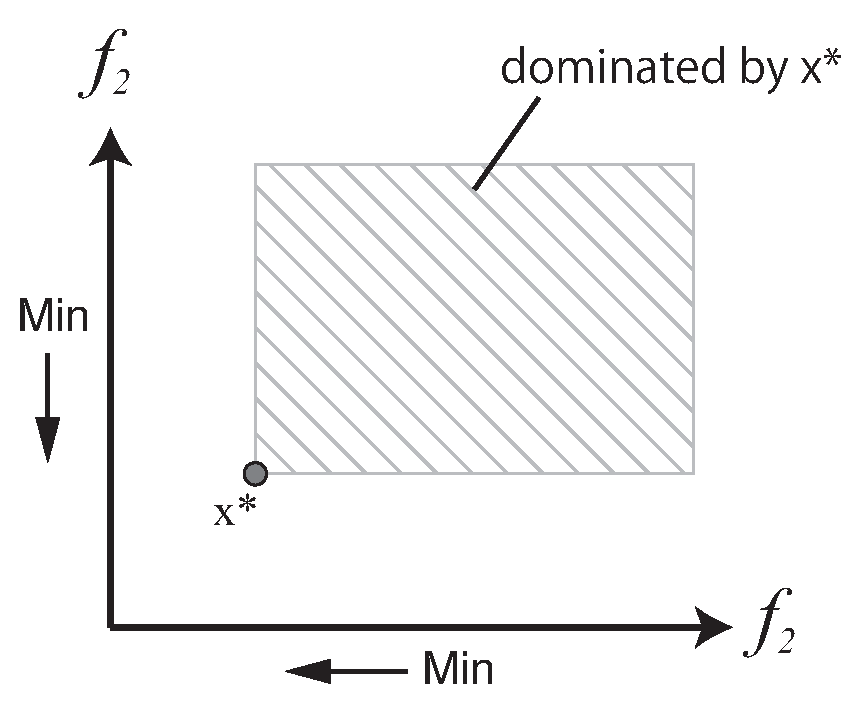
\includegraphics[width=0.9\linewidth]{../figures/dominance_image.eps}
\begin{center}
{\footnotesize (a) 通常の優越関係を用いた場合の支配領域}
\end{center}
\end{minipage}
\begin{minipage}{0.49\hsize}
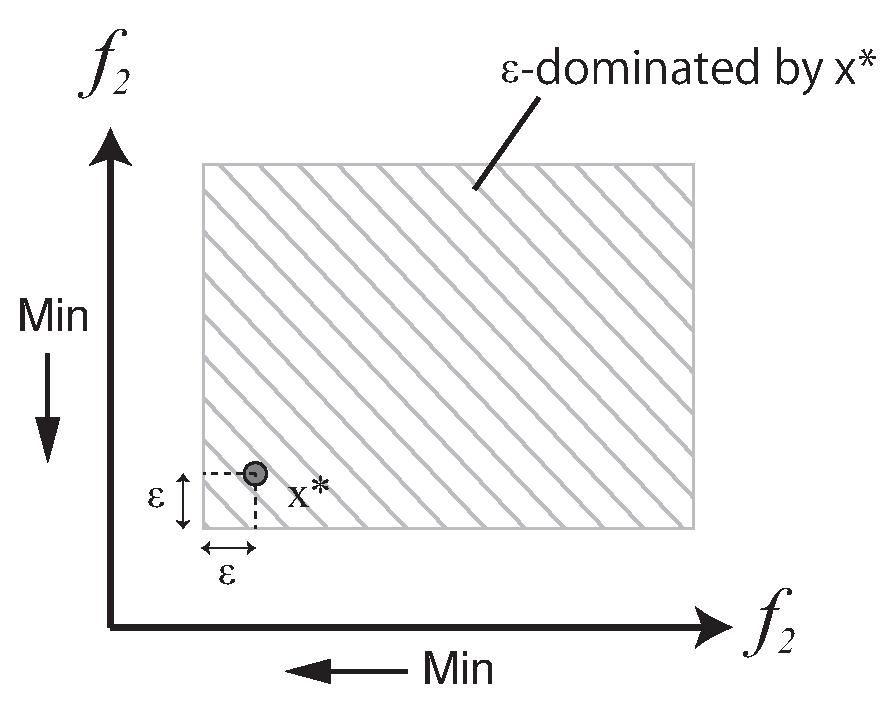
\includegraphics[width=0.9\linewidth]{../figures/epsilon-dominance_image.eps}
\begin{center}
{\footnotesize (b) $\epsilon$-dominanceを用いた場合の支配領域}
\end{center}
\end{minipage}
\end{tabular}
\caption{$\epsilon$-dominanceを用いた場合の支配領域の比較}
\label{epsilon_dominance_image}
\end{figure}

\Figref{epsilon_dominance_image}のように,$\epsilon$-dominanceを用いることで解の支配領域が増え,さらに増えた領域内では非劣解を一点のみ採用するため,非劣解の数が削減される.
削減した非劣解をアーカイブとして用いる手法が提案されており,多数目的最適化問題において収束性などの探索効率が向上することが示されている.

\clearpage

\item[目的関数空間の異なるスケールを目的関数に持つ問題に関する研究]\mbox{}\\
\quad Ishibuchiらによって,目的関数空間の離散化具合による影響評価が行われている\cite{Ishibuchi2012Effects}.
多目的組み合わせ最適化問題などでは,異なるケースの離散値を取る目的関数を持つことがあるが,この違いが進化にもたらす影響を評価し,粗い離散値を取る目的関数がある場合,その関数の最適化方向への探索効率が低下することが示されている.
これは,粗い離散値を取る目的関数がある場合,非劣解の数が著しく減少してしまうからである.
このような問題でも効率的に探索を行うため,Ishibuchiらは粗い離散値を取る目的関数値に擬似的に乱数を付与することで,非劣解の数を増加させる手法を提案している.

\end{description}

\section{設計変数空間の離散化に関する研究}
%\quad 設計変数空間の離散化に関する研究としては,BCGAではビット長を可変にした手法が提案されている.
%一方,RCGAでは設計変数空間の離散化に関する研究は,Kondoらの行った離散変数が進化に及ぼす影響評価があるが,離散化を用いた手法の提案はなされていない.
%
%
%\subsection{BCGAにおける設計変数空間の離散化を用いた効率的探索手法}
\begin{description}
\item[バイナリ型GAにおける設計変数のビット長が進化に与える影響]\mbox{}\\
\quad 設計変数空間の離散化に関する研究としては,主にバイナリ型遺伝的アルゴリズム(Binary-Coded Genetic Algorithms; BCGAs; バイナリ型GA)において研究が進められている.
バイナリ型GAは実数値GAと異なり,設計変数は0,1のバイナリビット列を持つアルゴリズムである.
したがって,バイナリビット列のビット長がの長さにより,設計変数の取り得る値の数は減少するため,ビット長の長さを変えることが設計変数の粒度の変更と等価となる.
バイナリ型GAにおいては,設計変数のビット長を短くするほど解の収束速度が向上することが報告されている\cite{Jaimes2005MRMOGA}.
これは,設計変数のビット長を短くすることで,設計変数空間が粗く離散化され,探索空間の縮小に繋がるためだと考えられている.
\Figref{discretization_sample}は,異なるビット長を用いた際の探索空間の違いを示しており,格子点が各ビット長を用いた際の探索点を表している.
\Figref{discretization_sample}からわかるようにビット長を短くすることで,設計変数空間が粗く離散化され探索空間が減少していることがわかる.
この性質を活かし,バイナリ型GAではビット長を探索の中で動的に変化させることで探索速度を向上させる手法が提案されている.

\begin{figure}[htbp]
\begin{center}
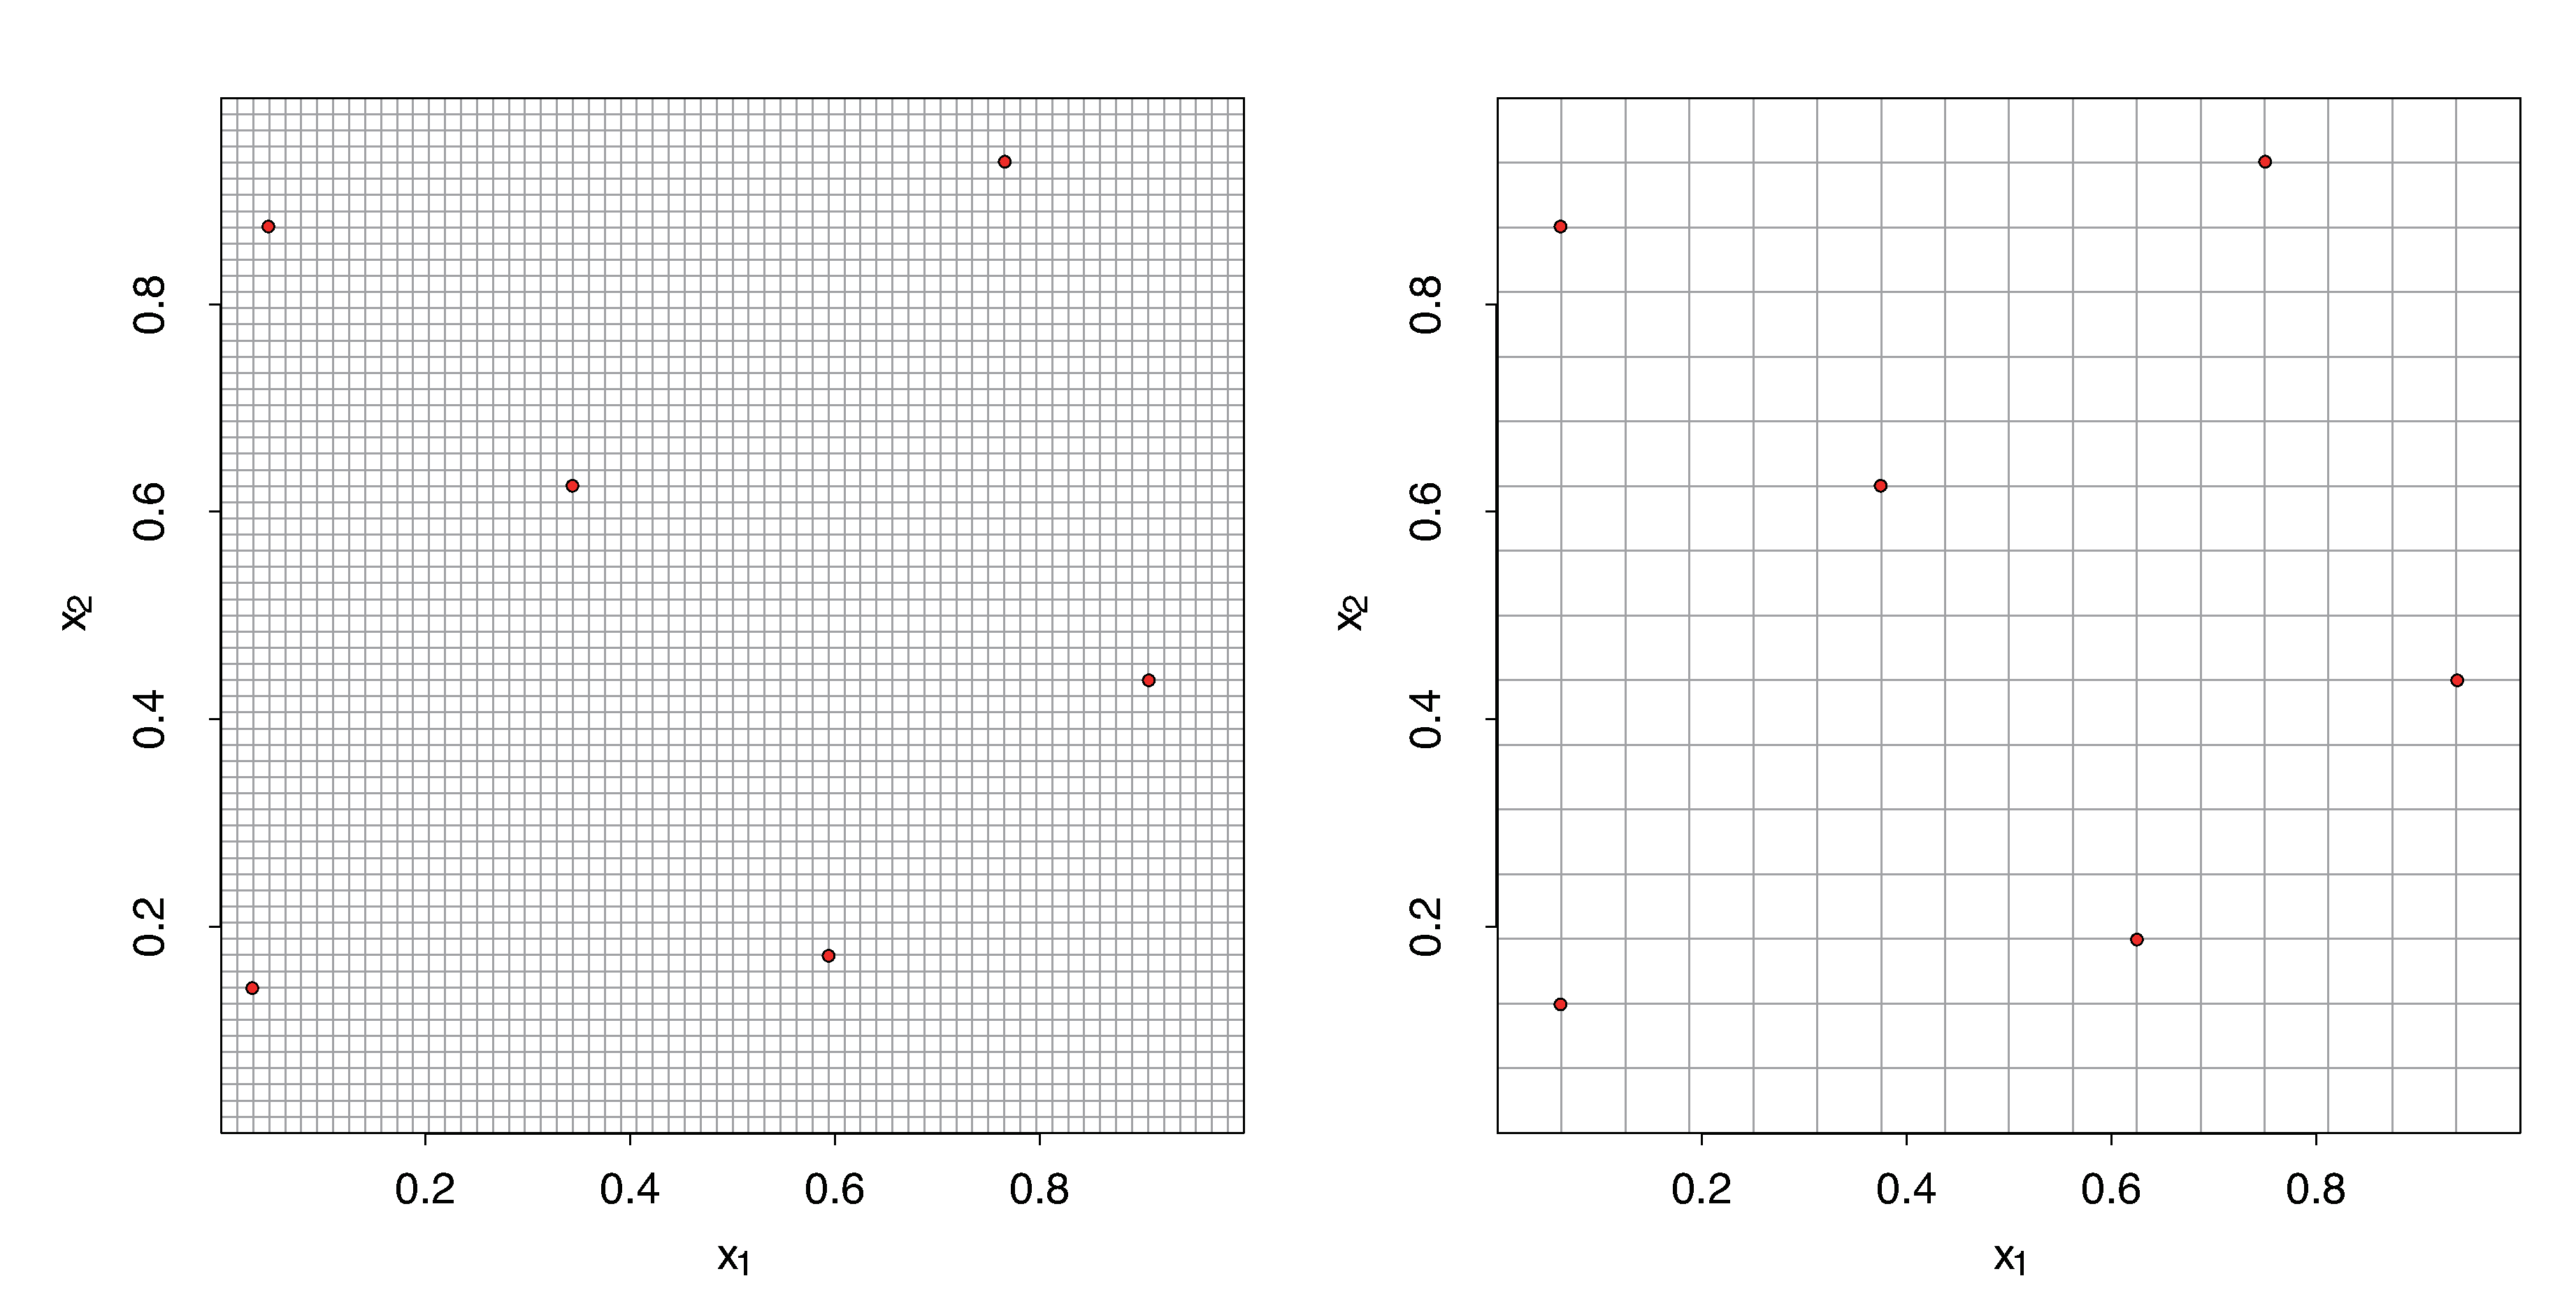
\includegraphics[width=0.9\linewidth]{../figures/discretization_sample.eps}
\end{center}
\caption[離散化による探索空間のイメージ図]{離散化による探索空間のイメージ図(左:ビット長6を用いた0-1の二変数の探索範囲 右:ビット長4を用いた0-1の二変数の探索範囲)}
\label{discretization_sample}
\end{figure}

%\quad BCGAにおける設計変数空間の離散化に関する研究としては,設計変数のビット長を短くするほど収束速度が向上することを前提にした手法がいくつか提案されている.

\item[BCGAにおける設計変数の可変ビット長に関する研究]\mbox{}\\
\quad 2005年にJaimesが提案したMultiple Resolutions Multiobjective Optimization Genetic Algorithm (MRMOGA)\cite{Jaimes2005MRMOGA}は,設計変数空間の離散化を取り入れた島モデル型BCGAである.
島モデル型のGAでは,複数個の集団を並行して最適化を行い,ある条件下で各集団の個体を別の集団に移す(移民)することで,最適化を行う手法である.
MRMOGAでは,各島(集団)で異なるビット長で表現される設計変数空間を考え,進化初期では少ないビット長(細かい離散化)で最適化を行い,徐々に長いビット長(細かい離散化)に変化させることで,収束速度の向上と多様性の維持を実現している.

\quad Kimらが提案したVariable Chromosome Length Genetic Algorithm (VCLGA)\cite{Kim2005Variable}もMRMOGA同様にビット長を可変にした構造最適化アルゴリズムを提案している.
VCLGAでは,少ないビット長で解が収束した場合,その解をエリートとして保存し,複数個の保存した解と同様の個体とランダムに作成した個体を用いて,ビット長を増加させ,再度計算を行う.

\quad MRMOGA,VCLGAともに短いビット長から徐々に長いビット長に変化させることで効率的探索を目指している.

%一方,RCGAではBCGAのような設計変数の解像度の動的制御や,設計変数の解像度が探索性能にあたえる影響についての議論はほとんどなされていなかった.
%\end{description}

\item[実数値GAにおける設計変数の離散化の影響評価に関する先行研究]\mbox{}\\
\quad 実数値GAにおいては上述のMRMOGAやVCLGAのように動的に設計変数を離散化する手法の研究はおろか,設計変数の離散化が進化に与える影響についてもあまり議論されてこなかった.
そこで,先行研究においては,実数値GAにおいて設計変数の離散化が進化に及ぼす影響をNSGA-IIと3つのベンチマーク問題を用いて評価した\cite{近藤2015}.
この研究では,設計変数の小数点以下の桁数を2,4,6,8,16桁に制御した場合のGD値とIGD値の推移を評価した.

\quad \Tabref{condition:pre}にはNSGA-IIの計算条件を,\Tabref{benchmark:pre}には先行研究で用いたベンチマーク問題と各問題で設定した集団サイズと世代数をまとめた.

\begin{table}[htbp]
\begin{tabular}{cc}
\begin{minipage}{0.49\hsize}
%\begin{table}[htbp]
\begin{center}
\caption{先行研究で用いた共通パラメータ}
\label{condition:pre}
\begin{tabular}{c|c}
\hline 
パラメータ& 数値 \\
\hline 
交叉率 & 1.0\\
突然変異率 & 1/n\\
$\eta_c$ & 30 \\
$\eta_m$ & 20 \\
試行回数 & 10\\
\end{tabular}
\end{center}
%\end{table}
\end{minipage}
\begin{minipage}{0.49\hsize}
%\begin{table}[htbp]
\begin{center}
\caption{先行研究で使用したベンチマーク問題ごとの計算条件}
\label{benchmark:pre}
\begin{tabular}{c|c|c|c}
\hline 
\quad & DTLZ2 & DTLZ3 & DTLZ4\\
\hline 
集団サイズ & 100 & 500 & 300\\
世代 & 100 & 200 & 100\\
\end{tabular}
\end{center}
%\end{table}
\end{minipage}
\end{tabular}
\end{table}

\quad \Figref{fig:gd}は,DTLZ2,3,4それぞれのGDの世代ごとの推移を示している.
\Figref{fig:gd}より,いずれの問題においても,赤色の線で示した最も粗く離散化されている2桁の結果が良い結果となっていることが分かる.
この結果からも,DTLZ問題では粗く離散化するほど収束性が向上する傾向があることが分かる.

\quad \Figref{fig:igd}は,DTLZ2,3,4それぞれのIGDの世代ごとの推移を示している.
\Figref{fig:igd}より,DTLZ2,3はGDの結果と同様に,最も粗く離散化されている2桁の結果が良い結果となっていることが分かる.
一方で,DTLZ4の結果は,2桁の結果が最も悪く,細かい粒度を持った8桁や16桁の結果が最も良い結果となっていることが確認できる.

\quad \Figref{non_a},\ref{non_b},\ref{non_c}は,2桁と16桁を用いた場合にDTLZ2,3,4それぞれで最終的に得られた非劣解の分布である.
\Figref{non_a}から,DTLZ2では,2桁と16桁で得られる非劣解の分布には大きな違いはないことが分かった.
\Figref{non_b}から,DTLZ3では,2桁のほうが明らかに最適化方向である原点方向に進化が進んでおり,明らかに収束性が高いことが分かる.
また,16桁の結果では,極付近に解が集中して分布していることが分かる.
これらの解はdominance-resistantsolutions (DRSs)\cite{Ikeda2001Failure}と呼ばれ,効率的な探索を妨げることが報告されている.
DRSsの詳細については後述する.
一方で,2桁の結果では,DRSsはほとんど発生していないことが分かる.
\Figref{non_c}から,DTLZ4では,2桁は局所的にしか解が得られていないことが分かる.
対照的に16桁は真のパレートフロントを覆うように非劣解が得られていることが分かる.
このことから,DTLZ4においては,粗い離散化をしすぎると解の多様性が失われてしまうことが考えられる.



%RCGAにおいては,KondoらによってNSGA-IIにおける設計変数の離散化による探索性能への影響評価がなされている\cite{}.

%この研究では\Tabref{benchmark_pre}で示す16個の多目的ベンチマーク問題を用いて,設計変数の小数点以下の桁数を2,4,6,8,16桁に制御した場合のGD値とIGD値の推移を評価した.
%\Tabref{benchmark}において,Problemは多目的ベンチマーク問題の名称を示している.
%また,Obj.,Var.,Con.,はそれぞれ各多目的ベンチマーク問題の目的関数の数,設計変数の数,制約条件の数を示す.
%MやNで示される目的関数の数,設計変数の数は,ユーザが任意に設定することができる.
%
%Separabilityは各設計変数が相関関係にあるか否かを示している.
%separableは相関関係なし,non-separableは相関関係ありを示す.
%separableな問題な場合,各設計変数の最適値は一意に定まる.
%一方で,non-separableな問題な場合,各設計変数の最適値は一意に定まらず,他の設計変数の値に応じて変化する.
%したがって,non-separableな問題のほうがseparableな問題に比べ,最適化が難しい傾向にある.
%
%Modalityは局所最適解があるか否かを示している.
%uniは単峰性の性質を持つ問題を示しており,局所最適解は存在せず大域的最適解のみが存在する問題である.
%一方で,multiは多峰性の性質を持つ問題を示しており,局所最適解を有する問題である.
%多峰性の性質を持つ問題は局所最適解を持つため,大域的最適解に収束しづらく,単峰性の性質を持つ問題と比較し,一般的に最適化が難しい傾向にある.
%
%Biasは目的関数空間において,解が偏りを持って生成されてしまう性質を有するか否かを示している.
%$\checkmark$で示される問題は,目的関数空間に解が射影される際,強い非線形性によって,解が局所的に集中しやすく,目的関数空間全体を覆うような多様性のある解を生成することが難しい問題である.
%したがって,Biasがある問題のほうが解の多様性を維持した最適解を得ることが難しい傾向にある.
%
%Geometryは真のパレート最適解の形状を示している.
%最適化手法によっては,真のパレート最適解の形状により得手不得手があるため,様々な形状の多目的ベンチマーク問題で性能を評価する必要がある.
%
%先行研究では,これら4つの特徴に基づいて代表的な問題を取り上げ影響の評価を行った.
%
%各ベンチマーク問題の構造は次章で詳しく述べる.
%
%%表の見方は第3章「多目的ベンチマーク問題」で述べた通りである.
%また,計算条件は\Tabref{tbl:pre:condition}に示す.
%$\eta_c$,$\eta_m$はそれぞれ交叉(SBX)と突然変異(polynomial mutation)の持つパラメータである.
%\Tabref{tbl:pre:gd},\ref{tbl:pre:igd}は,各ベンチマーク問題において小数点以下$2$桁,$4$桁,$6$桁,$8$桁,$16$桁で制御し最適化を行った場合のGDとIGDの平均値の推移を示している.
%表中に示すObj.は目的関数の数,Var.は設計変数の数,GenはGDとIGDの平均値を求めた世代数を示しており,各世代における最小値を太字で示している.
%
%
%\begin{table}[t]
%\fontsize{9.5pt}{9.5pt} \selectfont
%\tabcolsep = 1pt
%\centering
%\caption{Kondoらの研究で使用された多目的ベンチマーク問題}
%\vspace{0.1cm}
%\label{benchmark_pre}
%\begin{tabular}{cccc||cccc}
%\hline 
%Problem & Obj. &Var. & Con. & Separability & Modality & Bias & Geometry \\
%\hline 
%DTLZ2 & M & N & - & separable & uni & - & concave\\
%DTLZ3 & M & N & - & separable & multi & - & concave\\
%DTLZ4 & M & N & - & separable & uni & \checkmark & concave\\
%WFG2 & M & N & - & non-separable & multi & - & convex,disconnected\\
%WFG4 & M & N & - & separable & multi & - & concave\\
%WFG6 & M & N & - & non-separable & uni & - & concave\\
%WFG7 & M & N & - & separable & uni & \checkmark & concave\\
%UF2 & 2 & N & - & non-separable & multi & - & convex\\
%UF9& 3 & N & - & non-separable & multi & - & linear, disconnected\\
%CF2 & 2 & N & 1 & non-separable & multi & - & convex, disconnected\\
%CF7 & 2 & N & 2 & non-separable & multi & - & convex\\
%C1DTLZ3 & M & N & 1 & separable & multi & - & concave\\
%C2DTLZ2convex & M & N & 1 & separable & uni & - & convex, disconnected\\
%C3DTLZ1 & M & N & M & separable & multi & - & convex(feasible surface is PF)\\
%Car Side Impact & 3 & 7 & 10 & & & uncertain &\\
%Welded Beam Design& 2 & 4 & 4 & & & uncertain &\\
%\hline
%\end{tabular}
%\\
%{\scriptsize Obj. is the number of objectives; Var. is the number of variables; Con. is the number of constraints.}\\
%{\scriptsize $M$ is the user predefined number of objectives; $N$ is the user predefined number of variables.}\\
%{\scriptsize - indicates no value or no characteristic; \checkmark indicates that the problem has the characteristic.}\\
%{\scriptsize The Car Side Impact and Welded Beam Design problems have uncertain characterisics because of engineering problems.}
%\end{table}
%
%\begin{table}[htbp]
%\fontsize{11pt}{11pt} \selectfont
%\tabcolsep = 5pt
%\centering
%\caption{Values of the common parameters used in the experimental study.}
%\label{tbl:pre:condition}
%\begin{tabular}{c|c}
%\hline 
%parameter & value \\
%\hline 
%Crossover rate & 1.0\\
%Mutation rate & 1/n\\
%$\eta_c$ & 30 \\
%$\eta_m$ & 20 \\
%Trial & 10\\
%\end{tabular}
%\end{table}
%
%
%\begin{table*}[htbp]
%\centering
%\caption{Averaged GD at the 10th, half and final generation.
%Best case is highlighted in bold.}
%\fontsize{8pt}{8pt} \selectfont
%\tabcolsep = 1pt
%\label{tbl:pre:gd}
%\begin{tabular}{c|ccccc|c|c|c|c|c}
%\hline 
%problem & MG & PS & Obj. & Var. & Gen & 2-digit & 4-digit & 6-digit & 8-digit & 16-digit \\ 
%\cline{7-11}
%&&&&&&GD&GD&GD&GD&GD\\
%\hline
%\multirow{3}{*}{DTLZ2} &        &  & &     & 10 & \bf{1.647} &   1.756 &  1.766 &  1.759 & 1.759\\
%  				   & 100 & 100 & 3 & 38 & 50 &$\bf{1.576 \times 10^{-1}}$ &  $2.247 \times 10^{-1}$ & $2.414 \times 10^{-1}$ & $2.595 \times 10^{-1}$ & $2.565 \times 10^{-1}$\\
%				   &        &     &           &   &100 & $\bf{5.525 \times 10^{-2}}$ & $1.576 \times 10^{-1}$ & $9.490 \times 10^{-2}$ & $1.003 \times 10^{-1}$ & $1.011 \times 10^{-1}$\\
%\hline
%\multirow{3}{*}{DTLZ3} &     &&   &       & 10 & $\bf{2.191 \times 10^{3}}$ & $2.508 \times 10^{3}$ &  $2.518 \times 10^{3}$ & $2.512 \times 10^{3}$ & $2.508 \times 10^{3}$\\
%  				   & 200 & 500 & 3 & 38 &100 & $\bf{9.935 \times 10}$ & $2.230 \times 10^{2}$ &  $2.878 \times 10^{2}$ & $3.154 \times 10^{2}$ & $4.039 \times 10^{2}$\\
%				   &        &   &&     &200 & \bf{6.521} & $4.580 \times 10$ &  $5.622 \times 10$ & $6.196 \times 10$ & $6.669 \times 10$\\
%
%\hline
%\multirow{3}{*}{DTLZ4} &        &     &&  & 10 & $\bf{8.213 \times 10^{-1}}$ & 1.286 & 1.216 & 1.223 & 1.223\\
%  				   & 100 & 300 & 3&38& 50 & $\bf{1.910 \times 10^{-2}}$ & $5.531 \times 10^{-2}$ & $6.576 \times 10^{-2}$ & $6.889 \times 10^{-2}$ & $7.147 \times 10^{-2}$\\
%				   &        &     &&   &100 & $\bf{1.101 \times 10^{-2}}$ & $1.819 \times 10^{-2}$ & $2.320 \times 10^{-2}$ & $2.363 \times 10^{-2}$ & $2.522 \times 10^{-2}$\\
%\hline
%\multirow{3}{*}{UF2} &        &    &&   & 10 &$\bf{2.978 \times 10^{-1}}$ & $3.106 \times 10^{-1}$ & $3.149 \times 10^{-1}$ & $3.001 \times 10^{-1}$ & $3.001 \times 10^{-1}$\\
%  				   & 200 & 200 & 2 & 20 & 100 &$2.639 \times 10^{-2}$ & $\bf{2.312 \times 10^{-2}}$ & $2.362 \times 10^{-2}$ & $2.451 \times 10^{-2}$ & $2.640 \times 10^{-2}$\\
%				   &        &      &&  &200 & $1.573 \times 10^{-2}$ & $\bf{1.349 \times 10^{-2}}$ & $1.573 \times 10^{-2}$ & $1.532 \times 10^{-2}$ & $1.701 \times 10^{-2}$\\
%
%\hline
%\multirow{3}{*}{UF9} &        &      && & 10& 3.063 & 3.048 & 2.695 & \bf{2.684} & \bf{2.684}\\
%  				   & 300 & 200 & 3 &20 &150 & $6.940 \times 10^{-1}$ & $\bf{5.745 \times 10^{-1}}$ & $6.584 \times 10^{-1}$ & $6.003 \times 10^{-1}$ & $6.425 \times 10^{-1}$\\
%				   &        &      &&  &300   &$\bf{4.206 \times 10^{-1}}$ &  $4.518 \times 10^{-1}$ & $4.892 \times 10^{-1}$ & $4.470 \times 10^{-1}$ & $4.389 \times 10^{-1}$\\
%\hline
%\multirow{3}{*}{WFG2} &        &   &&  10  & 10 & $2.350 \times 10^{-1}$ & $\bf{2.218 \times 10^{-1}}$ & $2.428 \times 10^{-1}$ & $2.428 \times 10^{-1}$ & $2.428 \times 10^{-1}$\\
%  				   & 100 & 100 & 3 & ($k=6$) &50 & $\bf{6.324 \times 10^{-2}}$ & $7.273 \times 10^{-2}$ & $6.490 \times 10^{-2}$ & $7.088 \times 10^{-2}$ & $7.141 \times 10^{-2}$\\
%				   &        &      && ($l=4$) &100 & $4.277 \times 10^{-2}$ & $4.745 \times 10^{-2}$ & $4.516 \times 10^{-2}$ & $4.530 \times 10^{-2}$ & $\bf{4.220 \times 10 ^{-2}}$\\
%\hline
%\multirow{3}{*}{WFG4} &        &   &&  10  & 10 & $2.249 \times 10^{-1}$ & $2.178 \times 10^{-1}$ & $2.143 \times 10^{-1}$ & $\bf{2.134 \times 10^{-1}}$ & $\bf{2.134 \times 10 ^{-1}}$\\
%  				   & 100 & 100 & 3 & ($k=6$) & 50 & $9.867 \times 10^{-2}$ & $9.530 \times 10^{-2}$ & $9.935 \times 10^{-2}$ & $9.563 \times 10^{-2}$ & $\bf{9.510 \times 10 ^{-2}}$\\
%				   &        &     && ($l=4$)  &100 & $6.772 \times 10^{-2}$ & $6.628 \times 10^{-2}$ & $6.678 \times 10^{-2}$ & $\bf{6.619 \times 10^{-2}}$ & $6.654 \times 10 ^{-2}$\\
%\hline
%\multirow{3}{*}{WFG6} &        &  &&  10   & 10 & $3.896 \times 10^{-1}$ & $3.611 \times 10^{-1}$ & $3.592 \times 10^{-1}$ & $\bf{3.560 \times 10^{-1}}$ & $\bf{3.560 \times 10 ^{-1}}$\\
%  				   & 100 & 100 & 3 & ($k=6$) & 50  & $1.545 \times 10^{-1}$ & $\bf{1.432 \times 10^{-1}}$ & $1.590 \times 10^{-1}$ & $1.653 \times 10^{-1}$ & $1.653 \times 10^{-1}$\\
%				   &        &      && ($l=4$) &100  & $1.201 \times 10^{-1}$ & $\bf{1.114 \times 10^{-1}}$ & $1.276 \times 10^{-1}$ & $1.215 \times 10^{-1}$ & $1.215 \times 10^{-1}$\\
%\hline
%\multirow{3}{*}{WFG7} &        &   &&  10  & 10 & $3.525 \times 10^{-1}$ & $\bf{3.506 \times 10^{-1}}$ & $3.553 \times 10^{-1}$ & $3.602 \times 10^{-1}$ & $3.602 \times 10^{-1}$\\
%  				   & 100 & 100 & 3 & ($k=6$) &50 & $ 1.226 \times 10^{-1} $ & $1.086  \times 10^{-1}$ & $\bf{9.925  \times 10^{-2}}$ & $1.061  \times 10^{-1}$ & $1.061  \times 10^{-1}$\\
%				   &        &       && ($l=4$) &100 & $7.178 \times 10^{-2}$ & $\bf{5.886 \times 10^{-2}}$ & $6.009 \times 10^{-2}$ & $6.561 \times 10^{-2}$ & $6.517 \times 10^{-2}$\\
%\hline
%\multirow{3}{*}{CF2}&        &     &&  & 10 & $\bf{8.459 \times 10^{-1}}$ &  $9.424 \times 10^{-1}$ & $9.266 \times 10^{-1}$ & $9.583 \times 10^{-1}$ & $9.583 \times 10^{-1}$\\
%  				   & 200 & 300 &2 & 20 & 100 &$\bf{2.069 \times 10^{-1}}$ &  $2.539 \times 10^{-1}$ & $2.729 \times 10^{-1}$ & $2.795 \times 10^{-1}$ & $2.851 \times 10^{-1}$\\
%				   &        &     &&   &200 & $1.694 \times 10^{-1}$ & $\bf{1.500 \times 10^{-1}}$ & $1.987 \times 10^{-1}$ & $2.051 \times 10^{-1}$ & $1.964 \times 10^{-1}$\\
%\hline
%\multirow{3}{*}{CF7} &        &    &&   & 10 & $2.584 \times 10$ & $2.605 \times 10$ &  $\bf{2.359 \times 10}$ & $2.679 \times 10$ & $2.721 \times 10$\\
%  				   & 200 & 300 &2 & 20 &100 & \bf{1.044} & 1.329 &  1.242  & 2.232 & 1.792 \\
%				   &        &     &&   &200 & $\bf{7.834 \times 10^{-2}}$ &  $4.992 \times 10^{-1}$ & $4.602 \times 10^{-1}$ & $7.675 \times 10^{-1}$ & $6.057 \times 10^{-1}$\\
%
%\hline
%\multirow{3}{*}{C1DTLZ3} &       && &       & 10 &  $\bf{2.661 \times 10^{3}}$ & $2.829 \times 10^{3}$ &  $2.845 \times 10^{3}$ & $2.871 \times 10^{3}$ & $2.871 \times 10^{3}$\\
%                                          &300 & 100 &3 & 38 & 150 & $\bf{1.051 \times 10^{2}}$ & $2.214 \times 10^{2}$ &  $2.601 \times 10^{2}$ & $3.168 \times 10^{2}$ & $3.267 \times 10^{2}$\\
%				   &        &       && &300 &  $\bf{4.986 \times 10}$ & $1.012 \times 10^{2}$ &  $1.043 \times 10^{2}$ & $1.297 \times 10^{2}$ & $1.243 \times 10^{2}$\\
%\hline
%\multirow{3}{*}{C2DTLZ2} &  &&      &       & 10 & $\bf{4.041 \times 10}$ & $5.867 \times 10$ &  $7.045 \times 10$ & $7.017 \times 10$ & $7.017 \times 10$\\
%  				   & 300 & 100 & 3 & 38&150 & $\bf{1.091 \times 10^{-1}}$ &  $1.299 \times 10^{-1}$ & $1.160 \times 10^{-1}$ & $1.191 \times 10^{-1}$ & $1.114 \times 10^{-1}$\\
%		convex		   &        &     &&   &300 &  $\bf{9.363 \times 10^{-2}}$ & $9.723 \times 10^{-2}$ & $9.941 \times 10^{-2}$ & $9.688 \times 10^{-2}$ & $9.450 \times 10^{-2}$\\
%
%\hline
%\multirow{3}{*}{C3DTLZ1} &       && &       & 10 &  $1.163 \times 10^{3}$ & $1.166 \times 10^{3}$ &  $\bf{1.152 \times 10^{3}}$ & $\bf{1.152 \times 10^{3}}$ & $\bf{1.152 \times 10^{3}}$\\
%                                          &300 & 100 & 3 & 38 &150 & $\bf{2.497 \times 10^{2}}$ & $2.797 \times 10^{2}$ &  $3.001 \times 10^{2}$ & $4.157 \times 10^{2}$ & $3.801 \times 10^{2}$\\
%				   &        &    &&    &300 &  $\bf{1.721 \times 10^{2}}$ & $2.002 \times 10^{2}$ &  $2.144 \times 10^{2}$ & $2.304 \times 10^{2}$ & $2.587 \times 10^{2}$\\
%				   \hline
%\multirow{3}{*}{\scriptsize Car Side}&  &&      &       & 10 &$7.528 \times 10^{-2}$ & $7.492 \times 10^{-2}$ & $7.618 \times 10^{-2}$ & $7.269 \times 10^{-2}$ & $\bf{6.863 \times 10 ^{-2}}$\\
%  				   & 300 & 500 & 3 & 7 &150 &$\bf{2.753 \times 10^{-2}}$ &  $3.066 \times 10^{-2}$ & $3.167 \times 10^{-2}$ & $3.173 \times 10^{-2}$ & $3.003 \times 10^{-2}$\\
%		{\scriptsize Impact}		   &        &      &&  &300 & $\bf{2.602 \times 10^{-2}}$ & $2.720 \times 10^{-2}$ & $2.970 \times 10^{-2}$ & $2.826 \times 10^{-2}$ & $2.881 \times 10^{-2}$\\
%\hline
%\multirow{3}{*}{\scriptsize Welded Beam} & &&       &       & 10 &$\bf{1.247 \times 10^{-1}}$ & $6.547 \times 10^{-1}$ & $5.801 \times 10^{-1}$ & $5.850 \times 10^{-1}$ & $5.850 \times 10 ^{-1}$\\
%  				   & 300 & 500 & 2 & 4 &150 &$2.395 \times 10^{-3}$ &  $3.043 \times 10^{-3}$ & $2.330 \times 10^{-3}$ & $2.764 \times 10^{-3}$ & $\bf{2.071 \times 10^{-3}}$\\
%	{\scriptsize Design}			   &        &      &&  &300 & $2.094 \times 10^{-3}$ & $1.854 \times 10^{-3}$ & $1.159 \times 10^{-3}$ & $\bf{1.071 \times 10^{-3}}$ & $2.295 \times 10^{-3}$\\
%
%\hline			   
%\hline\end{tabular}
%\\
%{\footnotesize MG = the number of generation set; PS = the number of population size set.}\\
%{\footnotesize Obj. = the number of objectives; Var. = the number of variables.}\\
%{\footnotesize Gen = the generation that results were computed on.} \\
%{\footnotesize k = position parameter in WFG problems; l = distance parameter in WFG problems.}\\
%\end{table*}
%
%\begin{table*}[htbp]
%\centering
%\caption{Averaged IGD at the 10th, half and final generation.
%Best case is highlighted in bold.}
%\fontsize{8pt}{8pt} \selectfont
%\tabcolsep = 1pt
%\label{tbl:pre:igd}
%\begin{tabular}{c|ccccc|c|c|c|c|c}
%\hline 
%problem & MG & PS & Obj. & Var. & Gen & 2-digit & 4-digit & 6-digit & 8-digit & 16-digit \\ 
%\cline{7-11}
%&&&&&&IGD&IGD&IGD&IGD&IGD\\
%\hline
%
%\multirow{3}{*}{DTLZ2} &  &&      &       & 10 & \bf{1.261} & 1.269 & 1.278 &  1.264 & 1.264\\
%  				  &100 & 100 & 3 & 38 & 50 & $\bf{1.469 \times 10^{-1}}$ &  $1.662 \times 10^{-1}$ & $1.753 \times 10^{-1}$ & $1.782 \times 10^{-1}$ & $1.782 \times 10^{-1}$\\
%				   &        &   &&     &100 & $\bf{5.433 \times 10^{-2}}$ & $6.017 \times 10^{-2}$ & $6.096 \times 10^{-2}$ & $6.453 \times 10^{-2}$ & $6.213 \times 10^{-2}$\\
%\hline
%\multirow{3}{*}{DTLZ3} &      &&  &       & 10 & $\bf{1.657 \times 10^{3}}$ & $1.694 \times 10^{3}$ &  $1.685 \times 10^{3}$ & $1.647 \times 10^{3}$ & $1.666 \times 10^{3}$\\
%  				   &200 & 500 & 3 & 38 & 100 & $\bf{6.871 \times 10}$ & $1.545 \times 10^{2}$ &  $1.921 \times 10^{2}$ & $2.001 \times 10^{2}$ & $2.195 \times 10^{2}$\\
%				   &        &      &&  &200 & \bf{5.059} & $3.451 \times 10$ &  $4.000 \times 10$ & $4.369 \times 10$ & $4.607 \times 10$\\
%
%\hline
%\multirow{3}{*}{DTLZ4} &   &&     &       & 10 & \bf{1.174} & 1.257 & 1.241 & 1.236 & 1.236\\
%  				   &100 & 300  & 3 & 38 & 50 & $ 6.164 \times 10^{-1} $ & $3.498  \times 10^{-1}$ & $\bf{3.195  \times 10^{-1}}$ & $3.503  \times 10^{-1}$ & $3.517  \times 10^{-1}$\\
%				   &        &     &&   &100 & $5.803 \times 10^{-1}$ & $2.773 \times 10^{-1}$ & $2.794 \times 10^{-1}$ & $\bf{2.507 \times 10^{-1}}$ & $\bf{2.507 \times 10 ^{-1}}$\\
%\hline
%\multirow{3}{*}{UF2} &        &     &&       & 10 & $2.131 \times 10^{-1}$ & $\bf{2.125 \times 10^{-1}}$ & $2.256 \times 10^{-1}$ & $2.283 \times 10^{-1}$ & $2.283 \times 10^{-1}$\\
%  				   &200 & 200 & 2 & 20 & 100 & $\bf{4.521 \times 10^{-2}}$ & $4.646 \times 10^{-2}$ & $5.174 \times 10^{-2}$ & $5.228 \times 10^{-2}$ & $5.312 \times 10^{-2}$\\
%				   &        &    &&    &200 & $4.147 \times 10^{-2}$ & $\bf{3.917 \times 10^{-2}}$ & $4.591 \times 10^{-2}$ & $4.411 \times 10^{-2}$ & $4.534 \times 10^{-2}$\\
%
%\hline
%\multirow{3}{*}{UF9} &        &    &&        & 10 & 1.161 & 1.183 & \bf{1.069} & 1.102 & 1.102\\
%  				   &300 & 200 & 3 & 20 & 150 & $3.057 \times 10^{-1}$ & $\bf{2.840 \times 10^{-1}}$ & $3.077 \times 10^{-1}$ & $3.169 \times 10^{-1}$ & $3.145 \times 10^{-1}$\\
%				   &        &     &&   &300 & $\bf{2.272 \times 10^{-1}}$ &  $2.235 \times 10^{-1}$ & $2.487 \times 10^{-1}$ & $2.543 \times 10^{-1}$ & $2.537 \times 10^{-1}$\\
%\hline
%\multirow{3}{*}{WFG2} &      &&  &   10    & 10 & $4.981 \times 10^{-1}$ & $\bf{4.963 \times 10^{-1}}$ & $4.964 \times 10^{-1}$ & $4.964 \times 10^{-1}$ & $4.964 \times 10^{-1}$\\
%  				   &100 & 100 & 3 & ($k = 6$) & 50 & $3.452 \times 10^{-1}$ & $3.462 \times 10^{-1}$ & $3.307 \times 10^{-1}$ & $3.087 \times 10^{-1}$ & $\bf{3.072 \times 10 ^{-1}}$\\
%				   &        &   &&  ($l=4$)   &100 & $3.008 \times 10^{-1}$ & $2.945 \times 10^{-1}$ & $3.185 \times 10^{-1}$ & $\bf{2.699 \times 10^{-1}}$ & $2.713 \times 10 ^{-1}$\\
%\hline
%\multirow{3}{*}{WFG4} &      &&  &   10    & 10 &$4.941 \times 10^{-1}$ & $\bf{4.402 \times 10^{-1}}$ & $4.466 \times 10^{-1}$ & $4.638 \times 10^{-1}$ & $4.638 \times 10^{-1}$\\
%  				   &100 & 100 & 3 & ($k=6$) & 50 & $1.520 \times 10^{-1}$ & $1.477 \times 10^{-1}$ & $1.546 \times 10^{-1}$ & $1.465 \times 10^{-1}$ & $\bf{1.439 \times 10 ^{-1}}$\\
%				   &        &&&  ($l=4$)      &100 & $1.003 \times 10^{-1}$ & $9.719 \times 10^{-2}$ & $1.016 \times 10^{-1}$ & $9.837 \times 10^{-2}$ & $\bf{9.700 \times 10 ^{-2}}$\\
%\hline
%\multirow{3}{*}{WFG6} &       && &   10    & 10 & $4.857 \times 10^{-1}$ & $4.829 \times 10^{-1}$ & $4.589 \times 10^{-1}$ & $\bf{4.538 \times 10^{-1}}$ & $\bf{4.538 \times 10 ^{-1}}$\\
%  				   &100 & 100 & 3 & ($k=6$) & 50  & $1.834 \times 10^{-1}$ & $\bf{1.690 \times 10^{-1}}$ & $1.810 \times 10^{-1}$ & $1.846 \times 10^{-1}$ & $1.846 \times 10^{-1}$\\
%				   &        &  &&  ($l=4$)    &100  & $1.345 \times 10^{-1}$ & $\bf{1.247 \times 10^{-1}}$ & $1.346 \times 10^{-1}$ & $1.359 \times 10^{-1}$ & $1.359 \times 10^{-1}$\\
%\hline
%\multirow{3}{*}{WFG7} &       && &  10     & 10 & $5.090 \times 10^{-1}$ & $5.143 \times 10^{-1}$ & $5.014 \times 10^{-1}$ & $\bf{4.986 \times 10^{-1}}$ & $\bf{4.986 \times 10 ^{-1}}$\\
%  				   &100 & 100 & 3 &  ($k=6$)& 50 &  $ 2.361 \times 10^{-1} $ & $\bf{2.246  \times 10^{-1}}$ & $2.375  \times 10^{-1}$ & $2.345  \times 10^{-1}$ & $2.345  \times 10^{-1}$\\
%				   &        &    && ($l=4$)   &100 & $1.779 \times 10^{-1}$ & $1.701 \times 10^{-1}$ & $1.722 \times 10^{-1}$ & $\bf{1.658 \times 10^{-1}}$ & $1.664 \times 10 ^{-1}$\\				   			   
%\hline
%\multirow{3}{*}{CF2} &        &    &&   & 10 & $4.487 \times 10^{-1}$ & $\bf{4.484 \times 10^{-1}}$ & $4.807 \times 10^{-1}$ & $4.719 \times 10^{-1}$ & $4.715 \times 10^{-1}$\\
%  				   &200 & 300 & 2 & 20 & 100 & $1.074 \times 10^{-1}$ & $\bf{9.756 \times 10^{-2}}$ & $9.820 \times 10^{-2}$ & $1.023 \times 10^{-1}$ & $1.015 \times 10^{-1}$\\
%				   &   &&     &        &200 & $1.073 \times 10^{-1}$ & $9.058 \times 10^{-2}$ & $9.864 \times 10^{-2}$ & $9.672 \times 10^{-2}$ & $\bf{8.944 \times 10 ^{-2}}$\\
%\hline
%\multirow{3}{*}{CF7} &   &&     &       & 10 & $1.747 \times 10$ & $1.751 \times 10$ &  $\bf{1.720 \times 10}$ & $1.742 \times 10$ & $1.765 \times 10$\\
%  				   &200 & 300 & 2 & 20 & 100 & $\bf{4.949 \times 10^{-1}}$ & $5.319 \times 10^{-1}$ & $\bf{4.949 \times 10^{-1}}$ & $6.665 \times 10^{-1}$ & $7.408 \times 10^{-1}$\\
%				   &        &    &&    &200 & $5.217 \times 10^{-1}$ & $3.410 \times 10^{-1}$ & $3.300 \times 10^{-1}$ & $3.072 \times 10^{-1}$ & $\bf{2.853 \times 10 ^{-1}}$\\
%
%\hline
%\multirow{3}{*}{C1DTLZ3} &      &&  &     & 10 & $\bf{1.964 \times 10^{3}}$ & $2.052 \times 10^{3}$ &  $\bf{1.940 \times 10^{3}}$ & $1.950 \times 10^{3}$ & $1.950 \times 10^{3}$\\
%                                          &300 & 100 & 3 & 38 & 150 & $\bf{9.702 \times 10}$ & $1.660 \times 10^{2}$ &  $1.783 \times 10^{2}$ & $2.002 \times 10^{2}$ & $1.956 \times 10^{2}$\\
%				   &        &  &&      &300 &  $\bf{4.338 \times 10}$ & $7.928 \times 10$ &  $7.859 \times 10$ & $9.252 \times 10$ & $8.024 \times 10$\\
%\hline
%\multirow{3}{*}{C2DTLZ2} &   &&     &       & 10 & \bf{3.799} & 4.373 & 4.221 & 4.338 & 4.338\\
%  				   &300 & 100 & 3 & 38 & 150 & $\bf{7.416 \times 10^{-2}}$ & $8.165 \times 10^{-2}$ & $7.831 \times 10^{-2}$ & $7.594 \times 10^{-2}$ & $7.828 \times 10^{-2}$\\
%			convex	   &        &    &&    &300  & $\bf{7.111 \times 10^{-2}}$ & $7.861 \times 10^{-2}$ & $7.477 \times 10^{-2}$ & $7.388 \times 10^{-2}$ & $7.260 \times 10^{-2}$\\
%
%\hline
%\multirow{3}{*}{C3DTLZ1} &        &   &&    & 10 &  $7.123 \times 10^{2}$ & $6.939 \times 10^{2}$ &  $\bf{6.765 \times 10^{2}}$ & $6.938 \times 10^{3}$ & $6.938 \times 10^{3}$\\
%                                          &300 & 100 &3 & 38 & 150 & $\bf{5.704 \times 10}$ & $7.554 \times 10$ &  $8.131 \times 10$ & $9.100 \times 10$ & $8.776 \times 10^{2}$\\
%				   &        &    &&    &300 &  $\bf{1.921 \times 10}$ & $2.938 \times 10$ &  $3.119 \times 10$ & $3.399 \times 10$ & $3.508 \times 10$\\
%\hline
%\multirow{3}{*}{\scriptsize Car Side} &  &&      &       & 10 &$2.222 \times 10^{-1}$ & $1.836 \times 10^{-1}$ & $1.861 \times 10^{-1}$ & $2.025 \times 10^{-1}$ & $\bf{1.824 \times 10 ^{-1}}$\\
%  				   &300 & 500 & 3 & 7 & 150 &$2.896 \times 10^{-2}$ &  $2.954 \times 10^{-2}$ & $2.934 \times 10^{-2}$ & $2.926 \times 10^{-2}$ & $\bf{2.879 \times 10^{-2}}$\\
%	{\scriptsize Impact}			   &        &   &&     &300 & $2.289 \times 10^{-2}$ & $2.261 \times 10^{-2}$ & $2.230 \times 10^{-2}$ & $2.229 \times 10^{-2}$ & $\bf{2.258 \times 10^{-2}}$\\
%\hline
%\multirow{3}{*}{\scriptsize Welded Beam} &   &&     &       & 10 &$2.932 \times 10^{-1}$ & $2.986 \times 10^{-1}$ & $\bf{2.495 \times 10^{-1}}$ & $2.507 \times 10^{-1}$ & $2.507 \times 10 ^{-1}$\\
%  				   &300 & 500 & 2 & 4 & 150 &$6.491 \times 10^{-2}$ &  $6.480 \times 10^{-2}$ & $5.166 \times 10^{-2}$ & $4.184 \times 10^{-2}$ & $\bf{3.196 \times 10^{-2}}$\\
%	{\scriptsize Design}			   &        &     &&   &300 & $3.929 \times 10^{-2}$ & $\bf{1.808 \times 10^{-2}}$ & $4.589 \times 10^{-2}$ & $3.456 \times 10^{-2}$ & $1.863 \times 10^{-2}$\\			   
%\hline\end{tabular}
%\end{table*}
%
%\Tabref{tbl:pre:gd}より,WFG2,WFG4,Welded Beam Design問題を除く13の問題において,桁数が小さいものの方が(粗く離散化したほうが)最終的なGD値が小さくなっていることが分かる.
%GD値は小さいほど収束性が優れていることを示す指標であることから,桁数が小さいほど収束性が向上する傾向があることが分かった.
%特にDTLZ問題ではどの世代においても桁数が小さいほど収束性が向上する結果が得られた.
%また,収束性が向上しなかったWFG2,WFG4,Welded Beam Design問題では,設計変数空間の定義域が大きく,小数点以下の桁数を制御しても離散化の影響が小さいため,収束性が向上しなかったことが考えられる.
%さらに,各桁数制御と16桁の結果の間に統計的有意差が存在するかを調べるため,有意水準5\%でウィルコクソンの順位和検定を行った結果,DTLZ2-4,UF9,CF2,CF7,C1DTLZ3,C2DTLZ2 convex,C3DTLZ1,Welded Beam Design問題で有意差が確認された.
%
%\Tabref{tbl:pre:igd}より,DTLZ2,3,UF2,9,CDTLZ問題では,GDの結果同様,桁数が小さいもののほうが(粗く離散化したほうが)最終的なIGD値が小さくなっていることが分かる.
%IGD値は小さいほど収束性と多様性が優れていることを示す指標であることから,これらの問題では桁数が小さいほど多様性が向上する傾向があることが分かった.
%しかしながら,DTLZ4においては,桁数が高いもののほうが最終的に良好なIGD値を取っていることが分かる.
%DTLZ4はDTLZ2と同じような構造を持っているが,目的関数の位置を司る変数が$\alpha$($=100$)乗されており,非常に非線形性が強い問題となっている.
%そのため,感度が非常に高く,精細な探索が必要となる.
%このことから,DTLZ4では,多様性を維持して探索を行うためには,単に粗く探索を行うのではなく,必要最低限な粒度の探索が必要であることが分かる.
%
%次に離散化の影響が顕著に見られたDTLZ2,3,4について,GD,IGD値の世代ごとの推移と非劣解の分布を比較する.
%
%\Figref{fig:gd}は,DTLZ2,3,4それぞれのGDの世代ごとの推移を示している.
%\Figref{fig:gd}より,いずれの問題においても,赤色の線で示した最も粗く離散化されている2桁の結果が良い結果となっていることが分かる.
%この結果からも,DTLZ問題では粗く離散化するほど収束性が向上する傾向があることが分かる.
%
%\Figref{fig:igd}は,DTLZ2,3,4それぞれのIGDの世代ごとの推移を示している.
%\Figref{fig:igd}より,DTLZ2,3はGDの結果と同様に,最も粗く離散化されている2桁の結果が良い結果となっていることが分かる.
%一方で,DTLZ4の結果は,2桁の結果が最も悪く,細かい粒度を持った8桁や16桁の結果が最も良い結果となっていることが確認できる.
%
%\Figref{non_a},\ref{non_b},\ref{non_c}は,2桁と16桁を用いた場合にDTLZ2,3,4それぞれで最終的に得られた非劣解の分布である.
%\Figref{non_a}から,DTLZ2では,2桁と16桁で得られる非劣解の分布には大きな違いはないことが分かった.
%\Figref{non_b}から,DTLZ3では,2桁のほうが明らかに最適化方向である原点方向に進化が進んでおり,明らかに収束性が高いことが分かる.
%また,16桁の結果では,極付近に解が集中して分布していることが分かる.

%
%\clearpage
%
\begin{figure*}[h]
\begin{tabular}{cc}
%\centering
\begin{minipage}{0.32\hsize}
%\begin{center}
%{\normalsize (A) DTLZ2}
%\end{center}
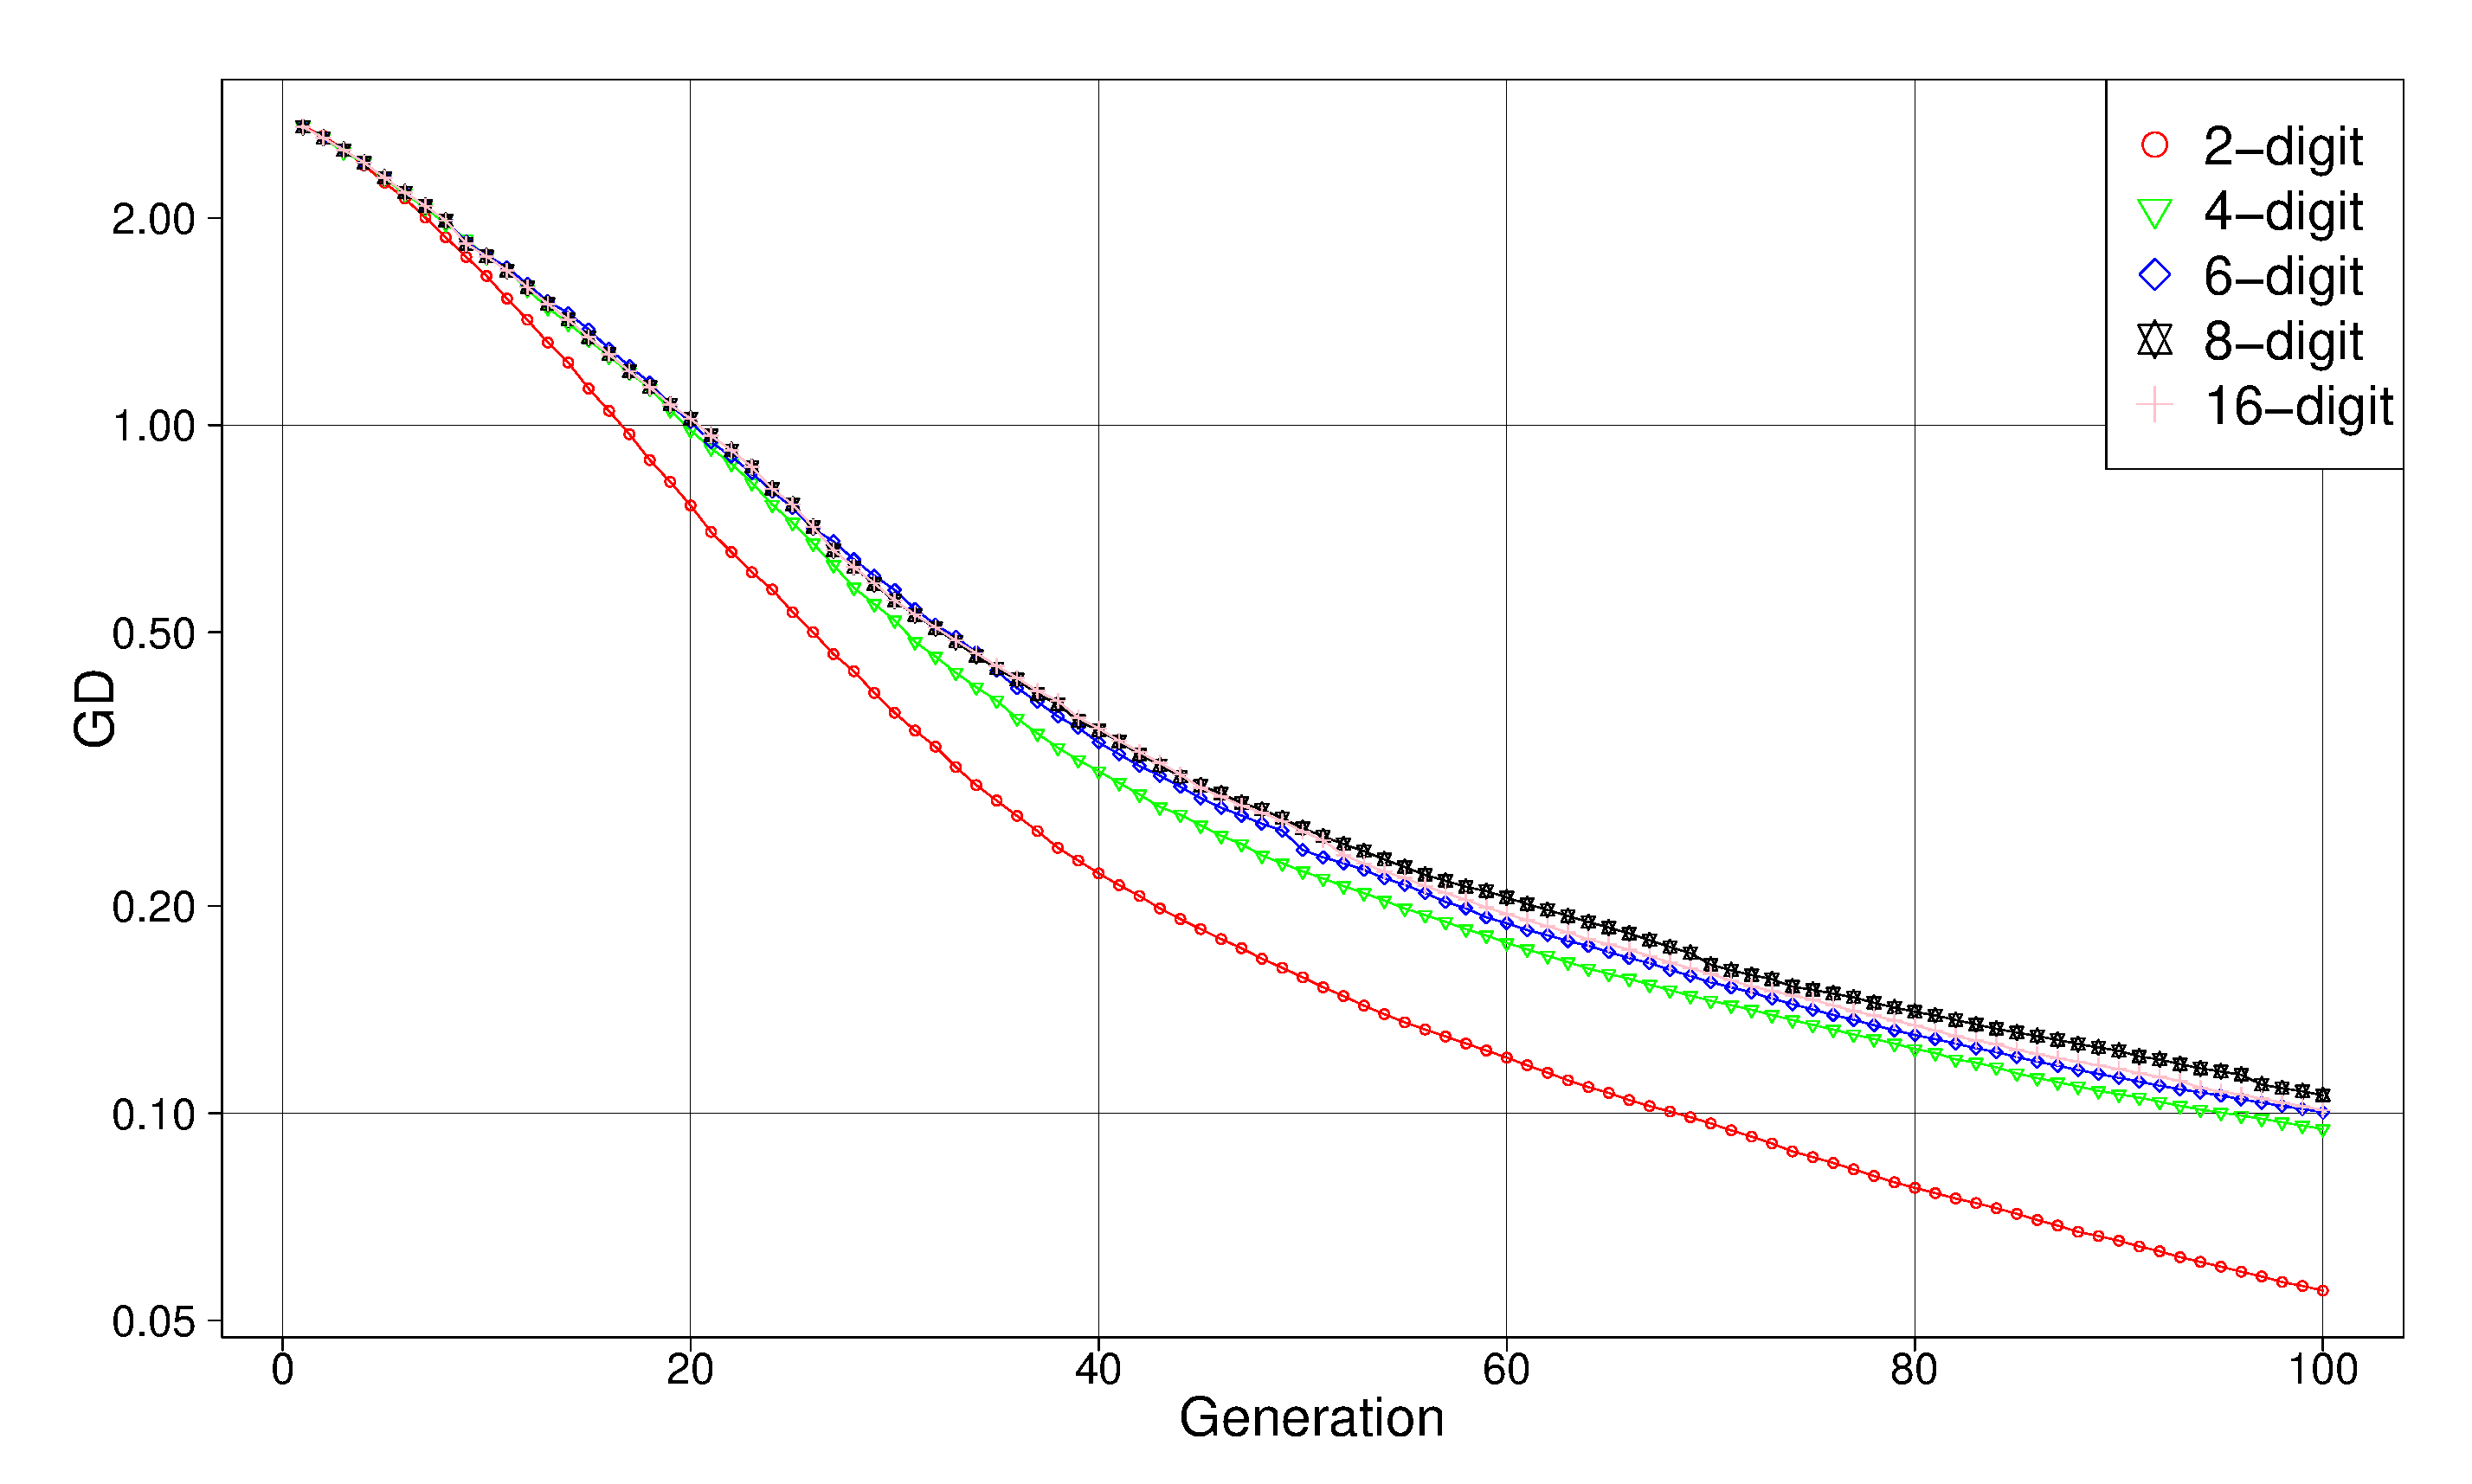
\includegraphics[width=1\linewidth]{../figures/DTLZ2_GD.eps}
%\setlength{\abovecaptionskip}{-8mm}
%\setlength{\belowcaptionskip}{-5mm}
%\caption{a}
\begin{center}
{\footnotesize (a) DTLZ2}
\end{center}
%\centering
\end{minipage}
%\hspace{-1mm}
\begin{minipage}{0.32\hsize}
%\begin{center}
%{\normalsize (B) DTLZ3}
%\end{center}
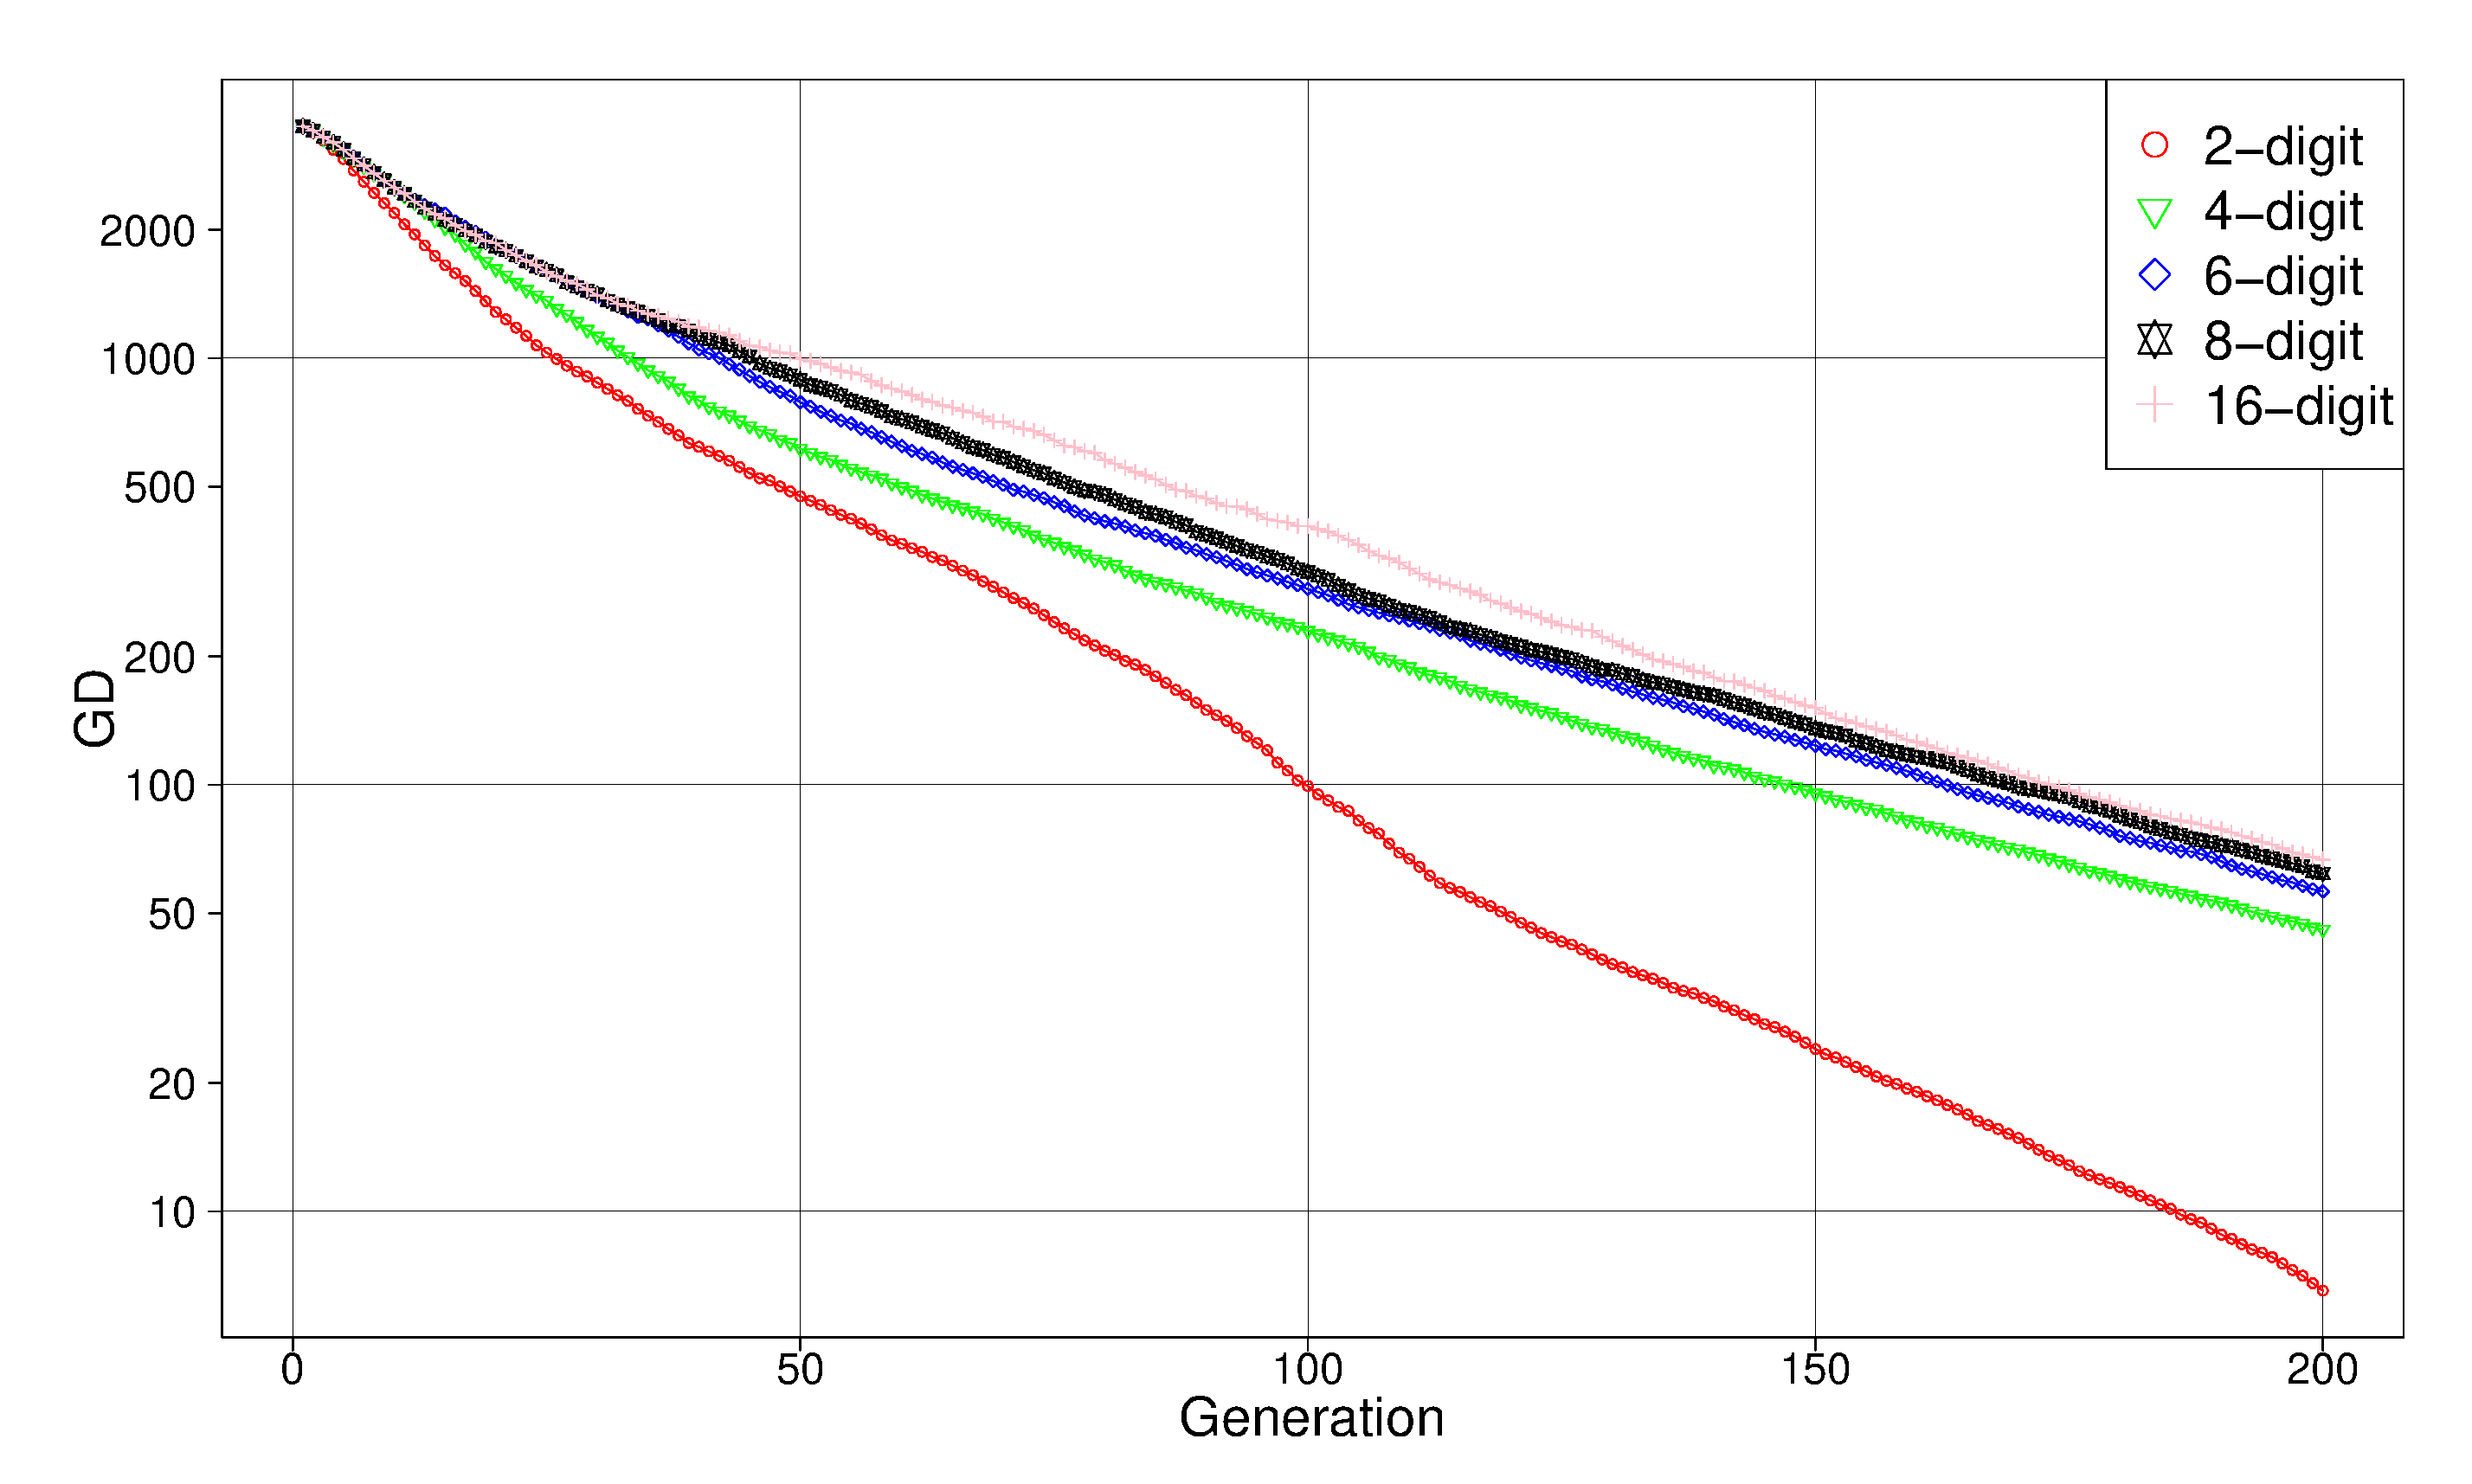
\includegraphics[width=1\linewidth]{../figures/DTLZ3_GD_pre.eps}
%\setlength{\abovecaptionskip}{-8mm}
%\setlength{\belowcaptionskip}{-5mm}
%\caption{a}
\begin{center}
{\footnotesize (b) DTLZ3}
\end{center}
%\centering
\end{minipage}
\begin{minipage}{0.32\hsize}
%\begin{center}
%{\normalsize (C) DTLZ4}
%\end{center}
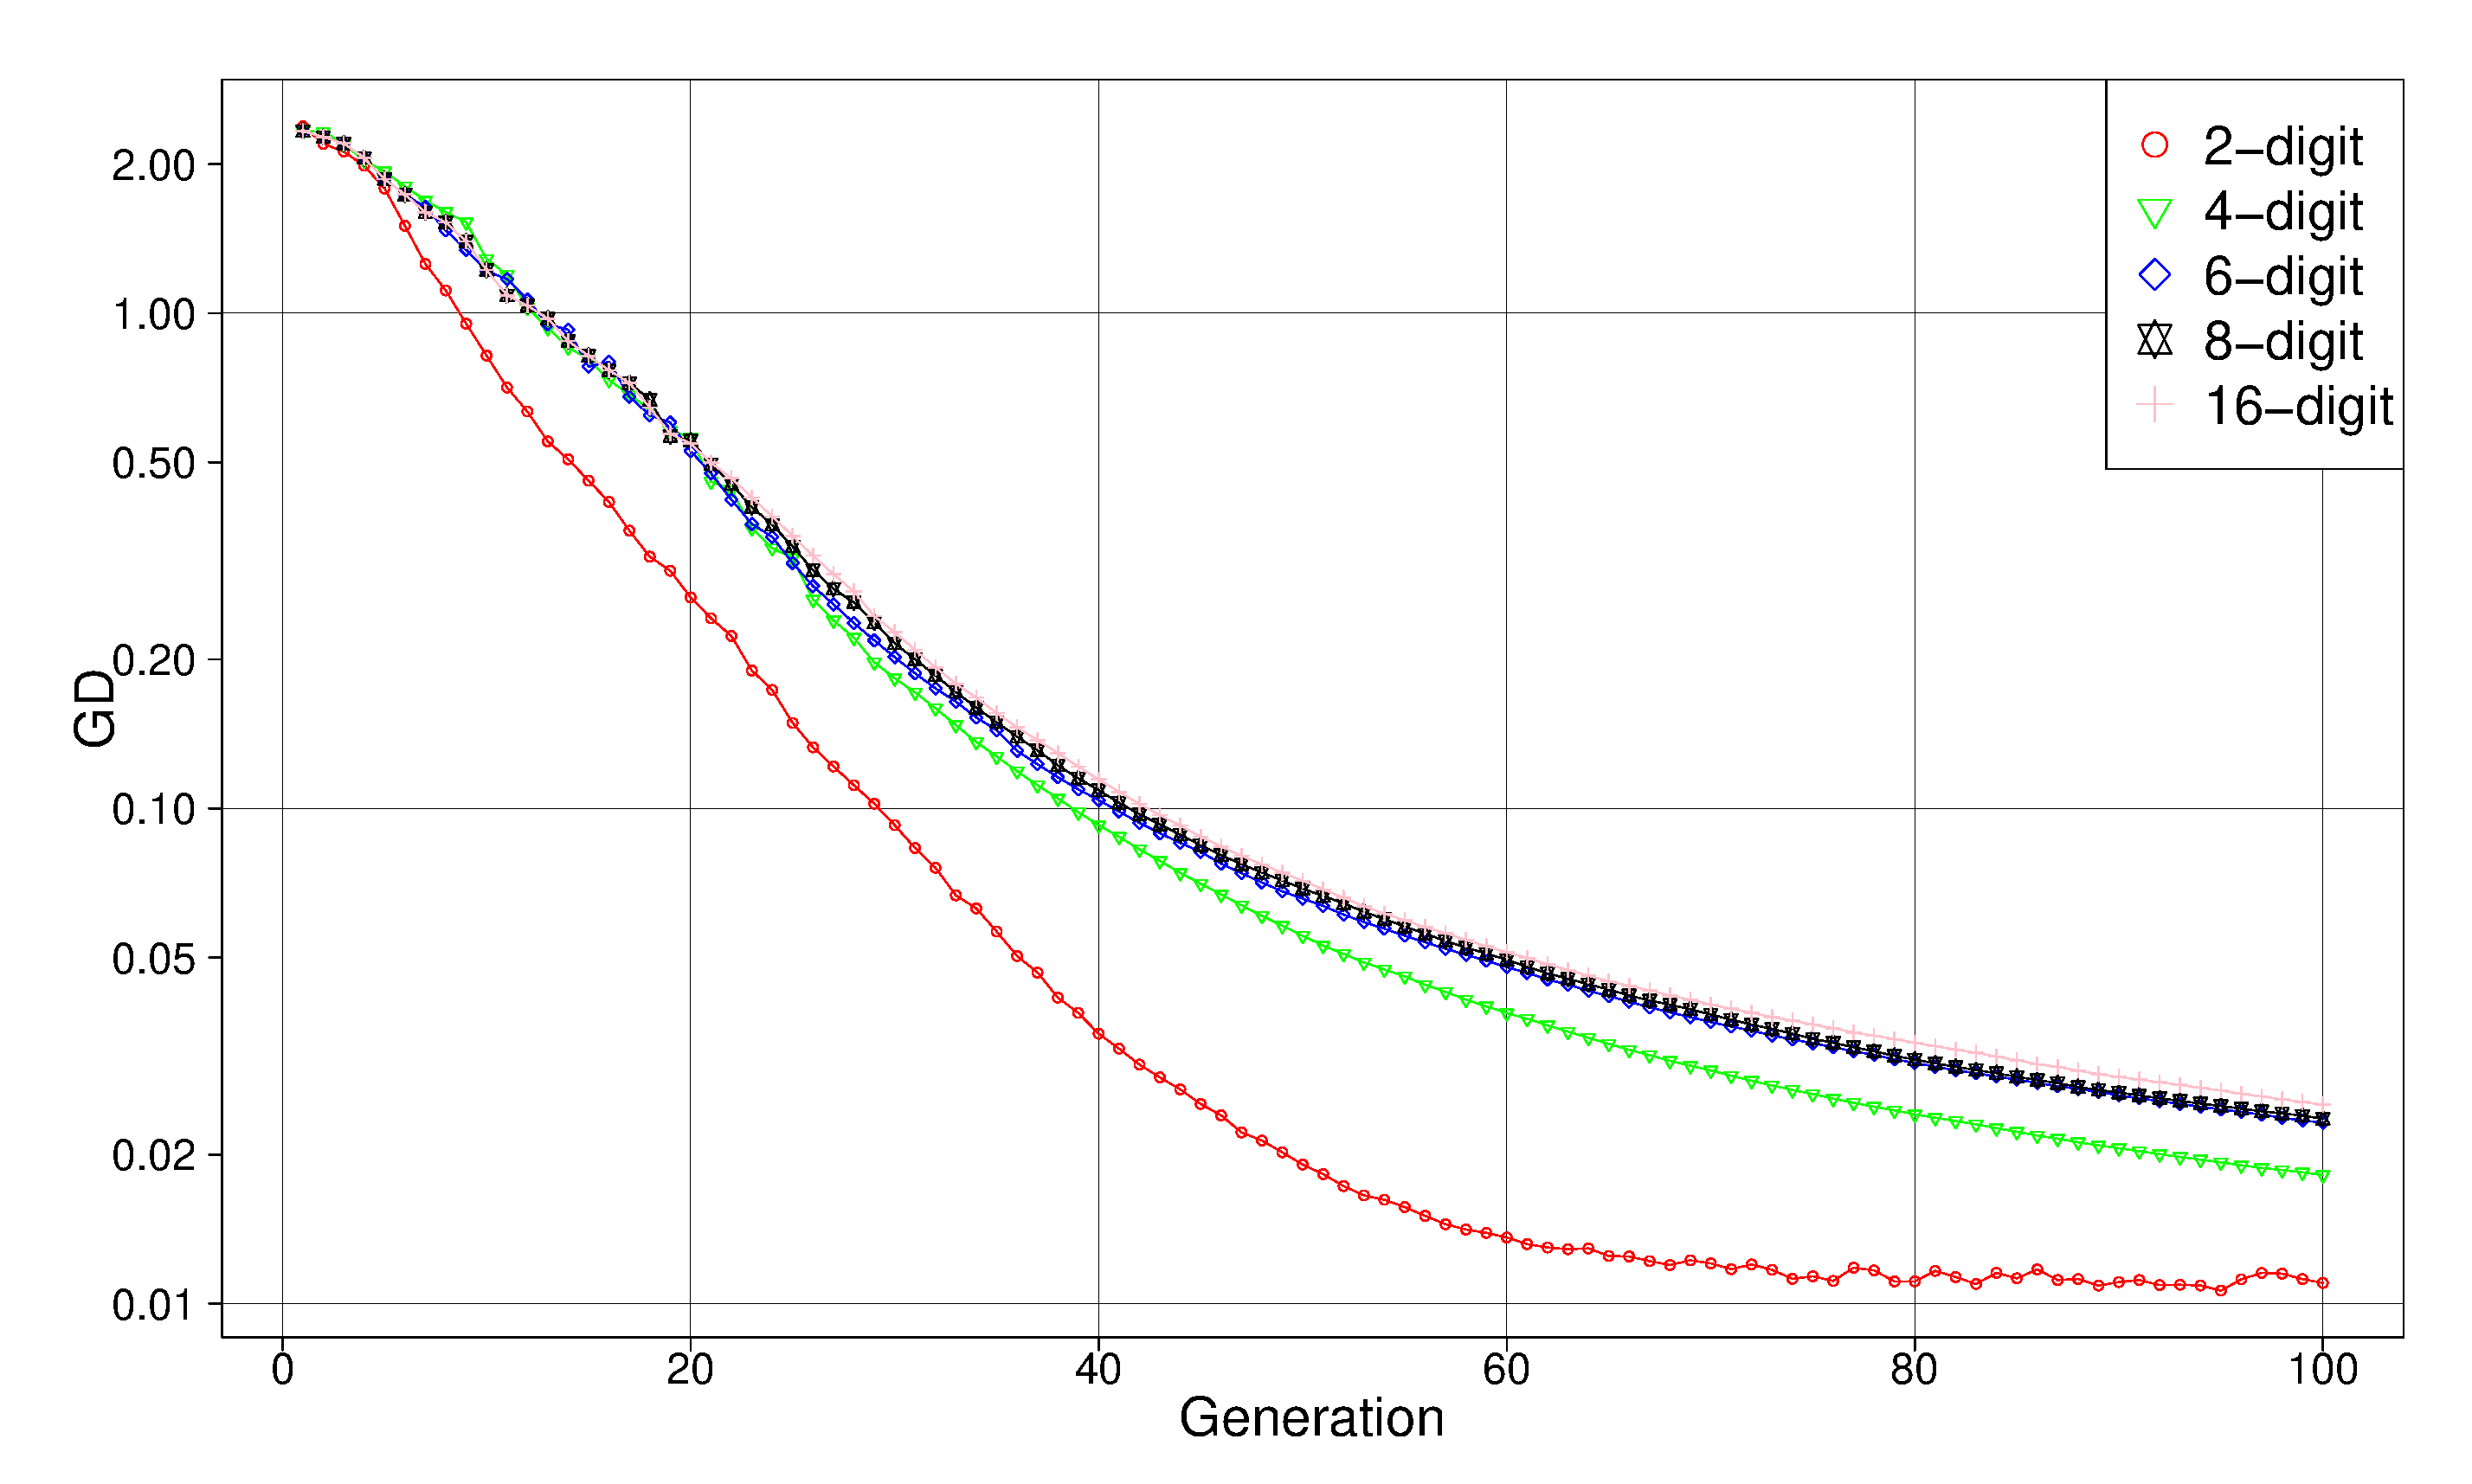
\includegraphics[width=1\linewidth]{../figures/DTLZ4_GD.eps}
%\setlength{\abovecaptionskip}{-8mm}
%\setlength{\belowcaptionskip}{-5mm}
%\caption{a}
\begin{center}
{\footnotesize (c) DTLZ4}
\end{center}
\end{minipage}
\end{tabular}
\caption{DTLZ2-4におけるGDの推移(NSGA-II)}
\label{fig:gd}
%\setlength\textfloatsep{-5mm}
\end{figure*}

%\vspace{-0.2in}

\begin{figure*}[htbp]
\begin{tabular}{cc}
\begin{minipage}{0.32\hsize}
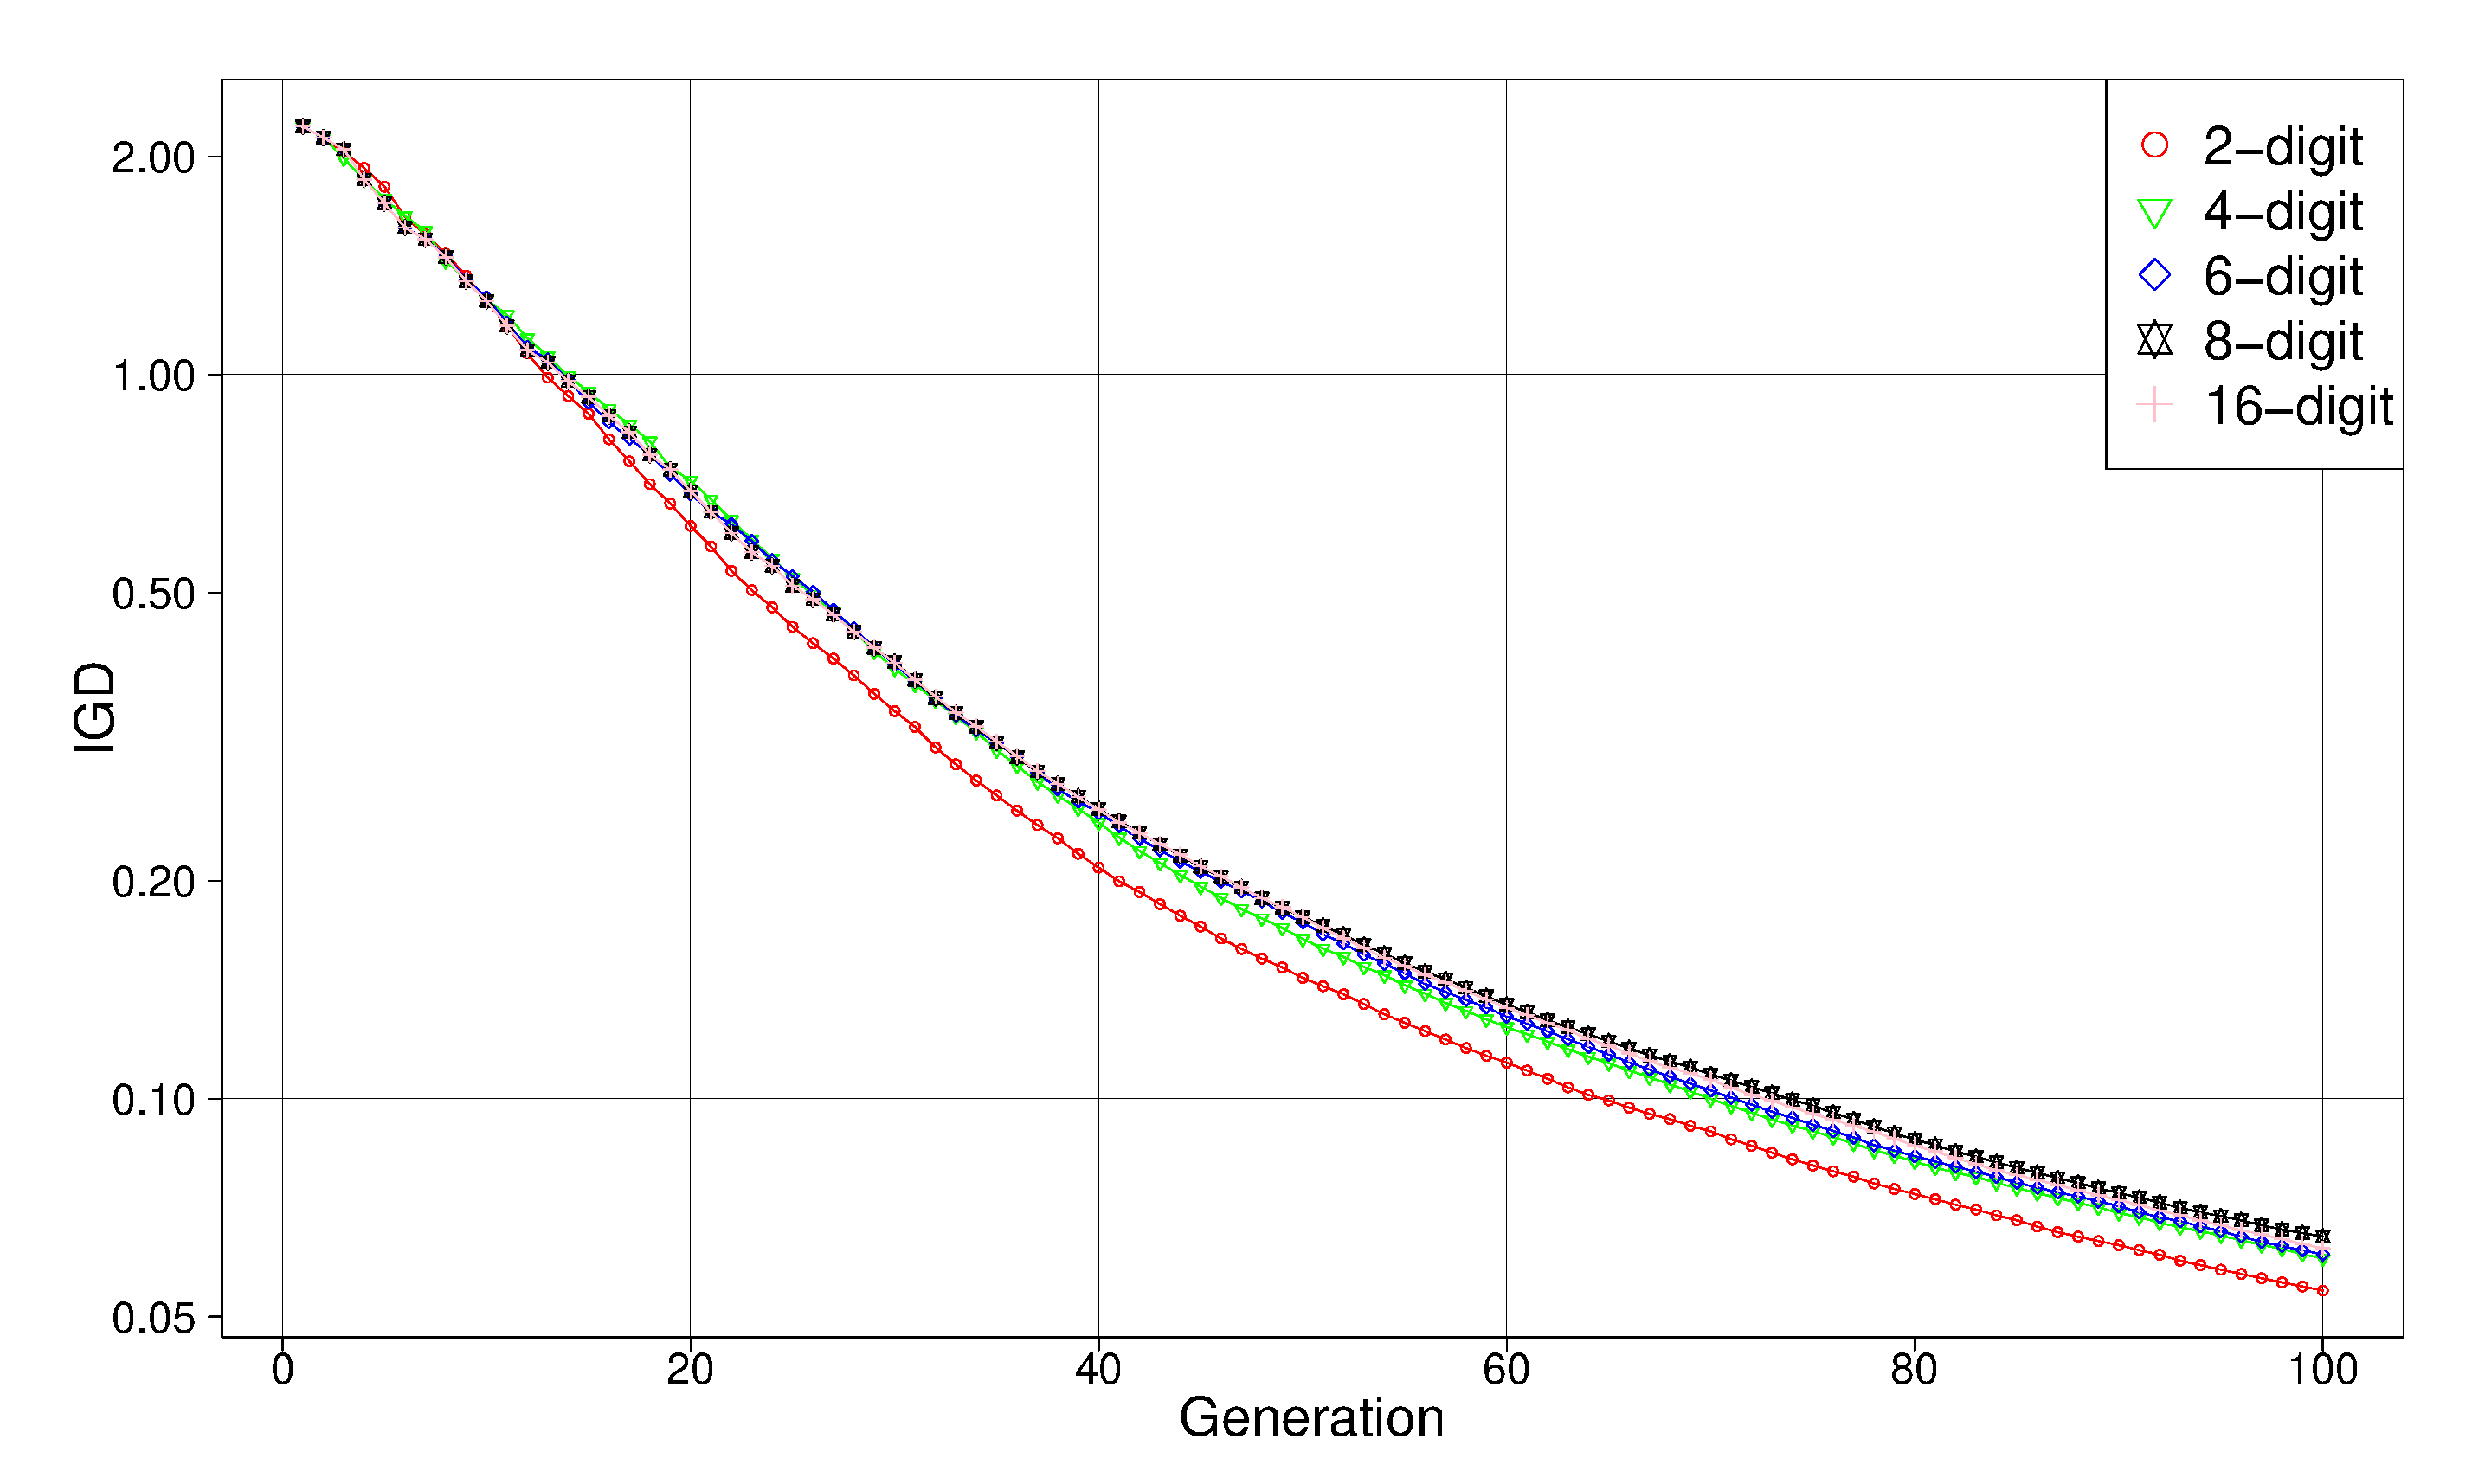
\includegraphics[width=1\linewidth]{../figures/DTLZ2_IGD.eps}
%\setlength{\abovecaptionskip}{-8mm}
%\setlength{\belowcaptionskip}{-5mm}
%\caption{a}
\begin{center}
{\footnotesize (a) DTLZ2}
\end{center}
\end{minipage}
%\hspace{-1mm}
\begin{minipage}{0.32\hsize}
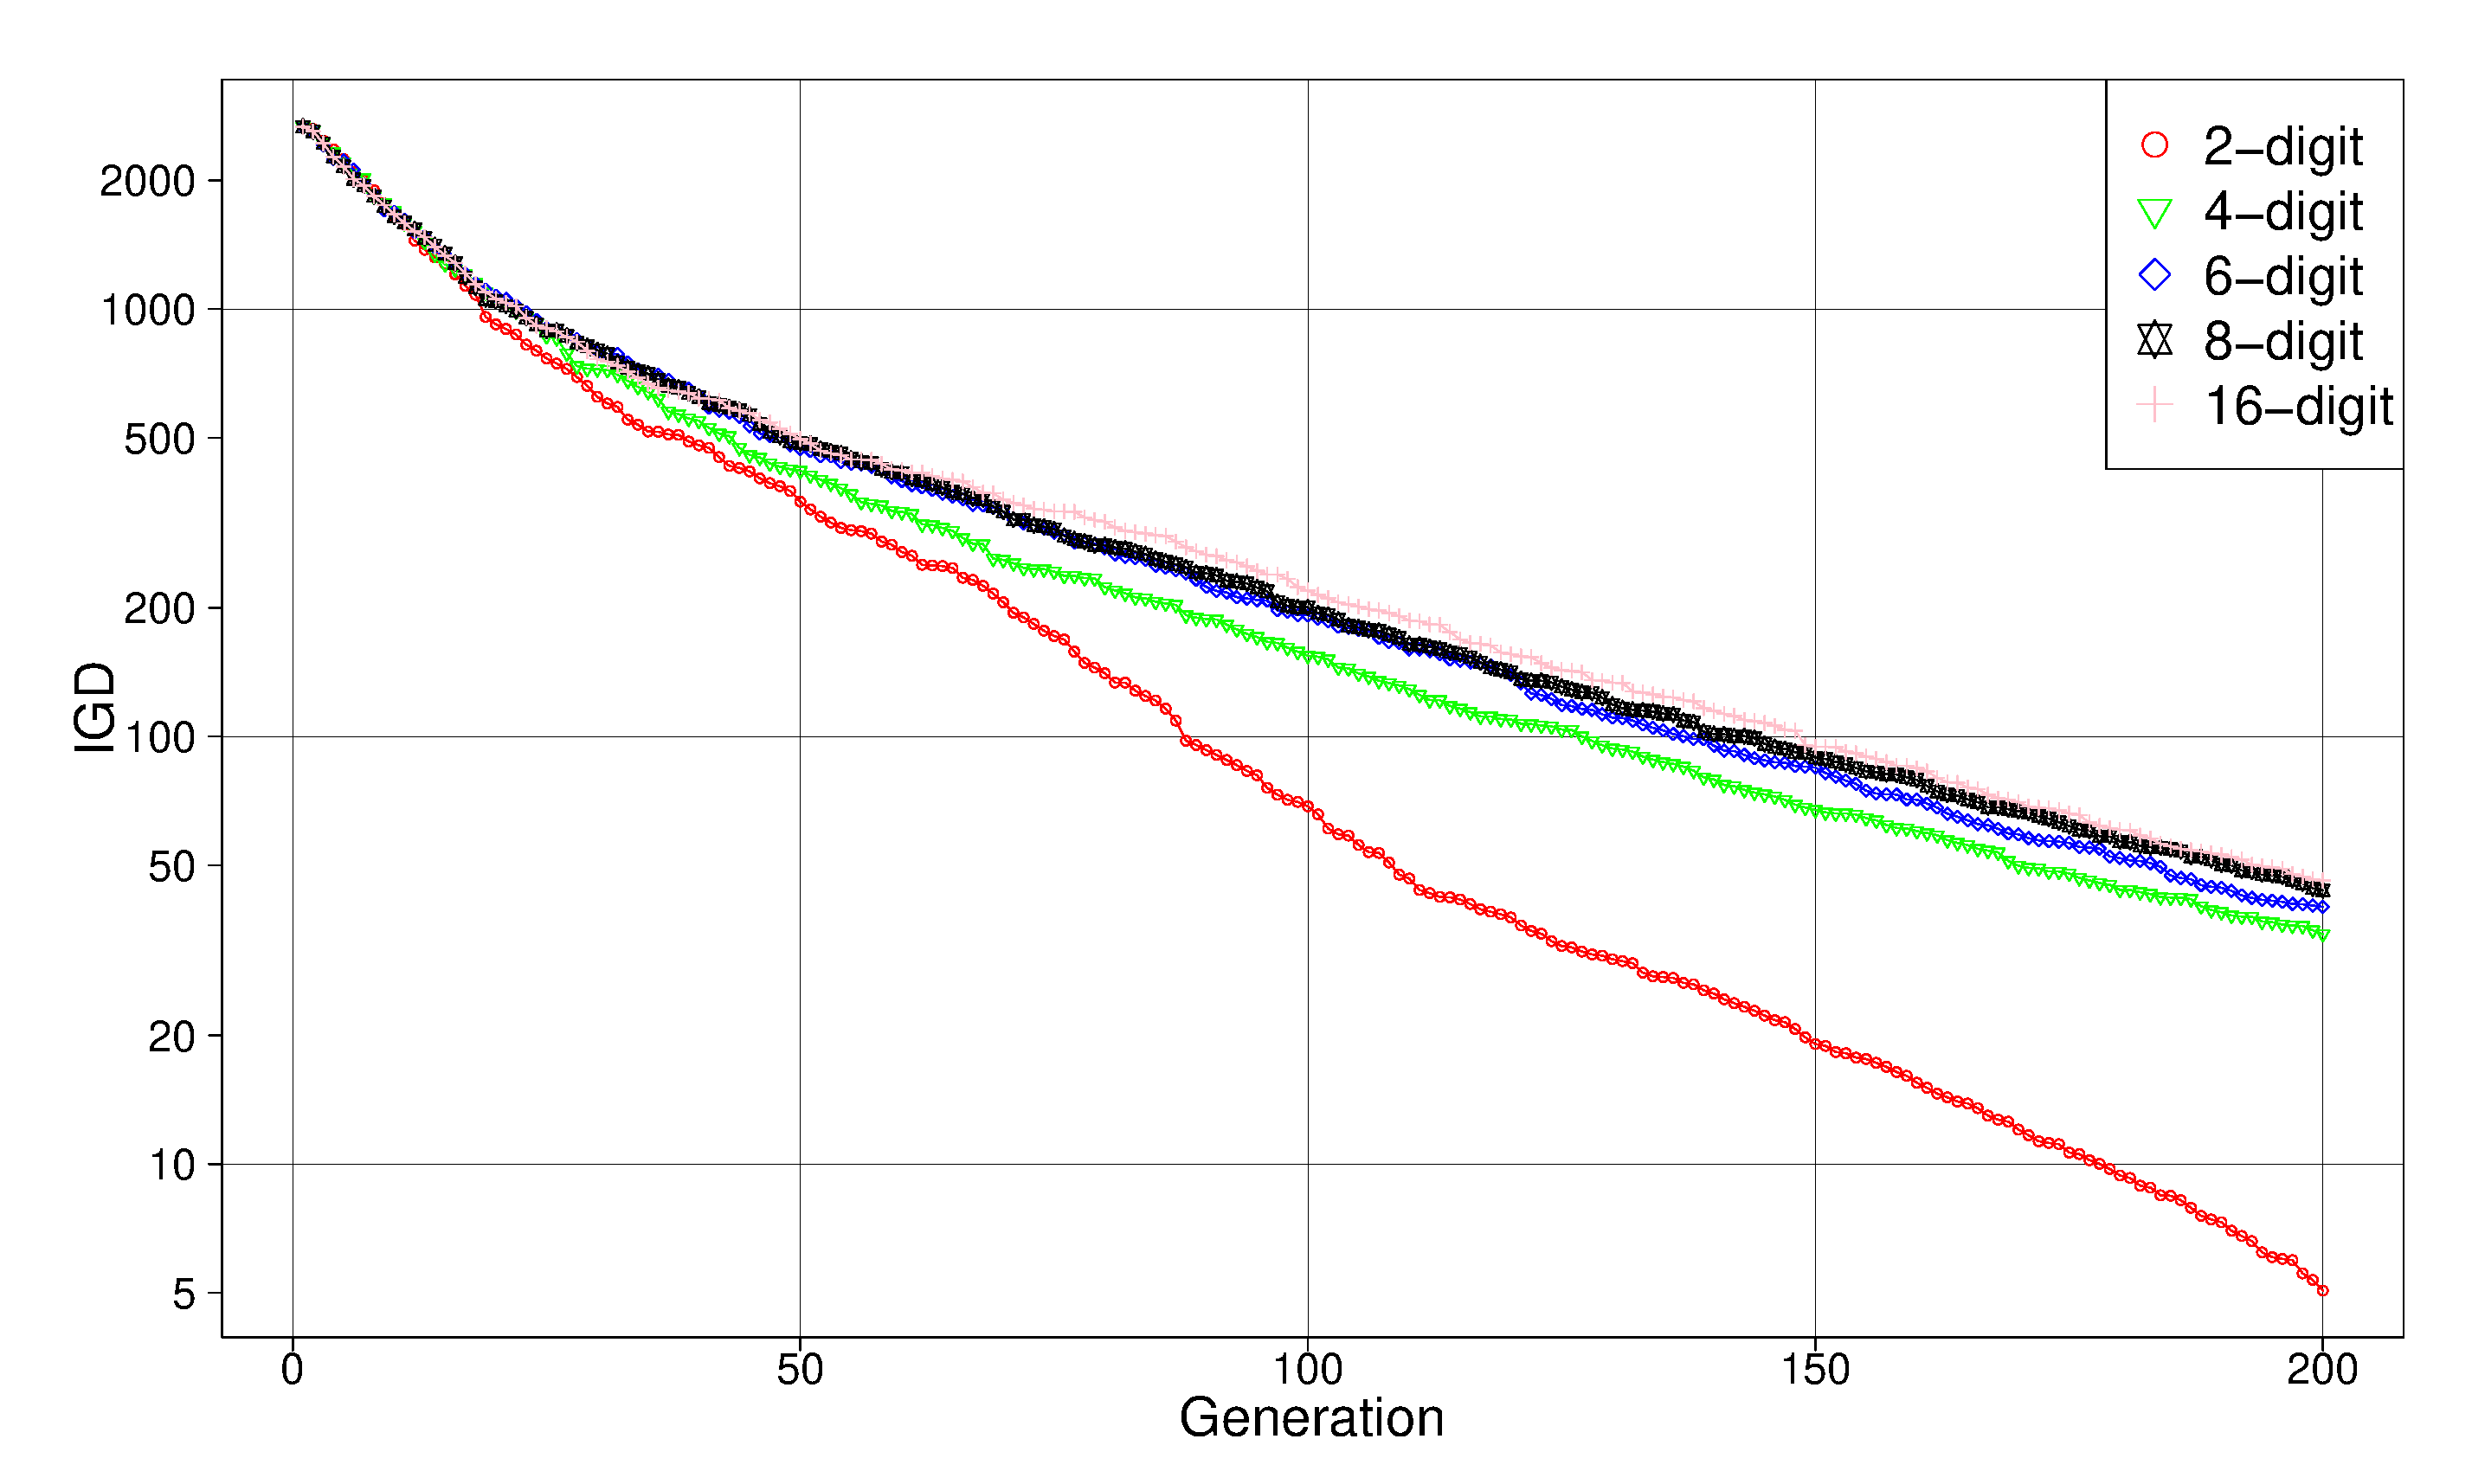
\includegraphics[width=1\linewidth]{../figures/DTLZ3_IGD_pre.eps}
%\setlength{\abovecaptionskip}{-8mm}
%\setlength{\belowcaptionskip}{-5mm}
%\caption{a}
\begin{center}
{\footnotesize (b) DTLZ3}
\end{center}
\end{minipage}
\begin{minipage}{0.32\hsize}
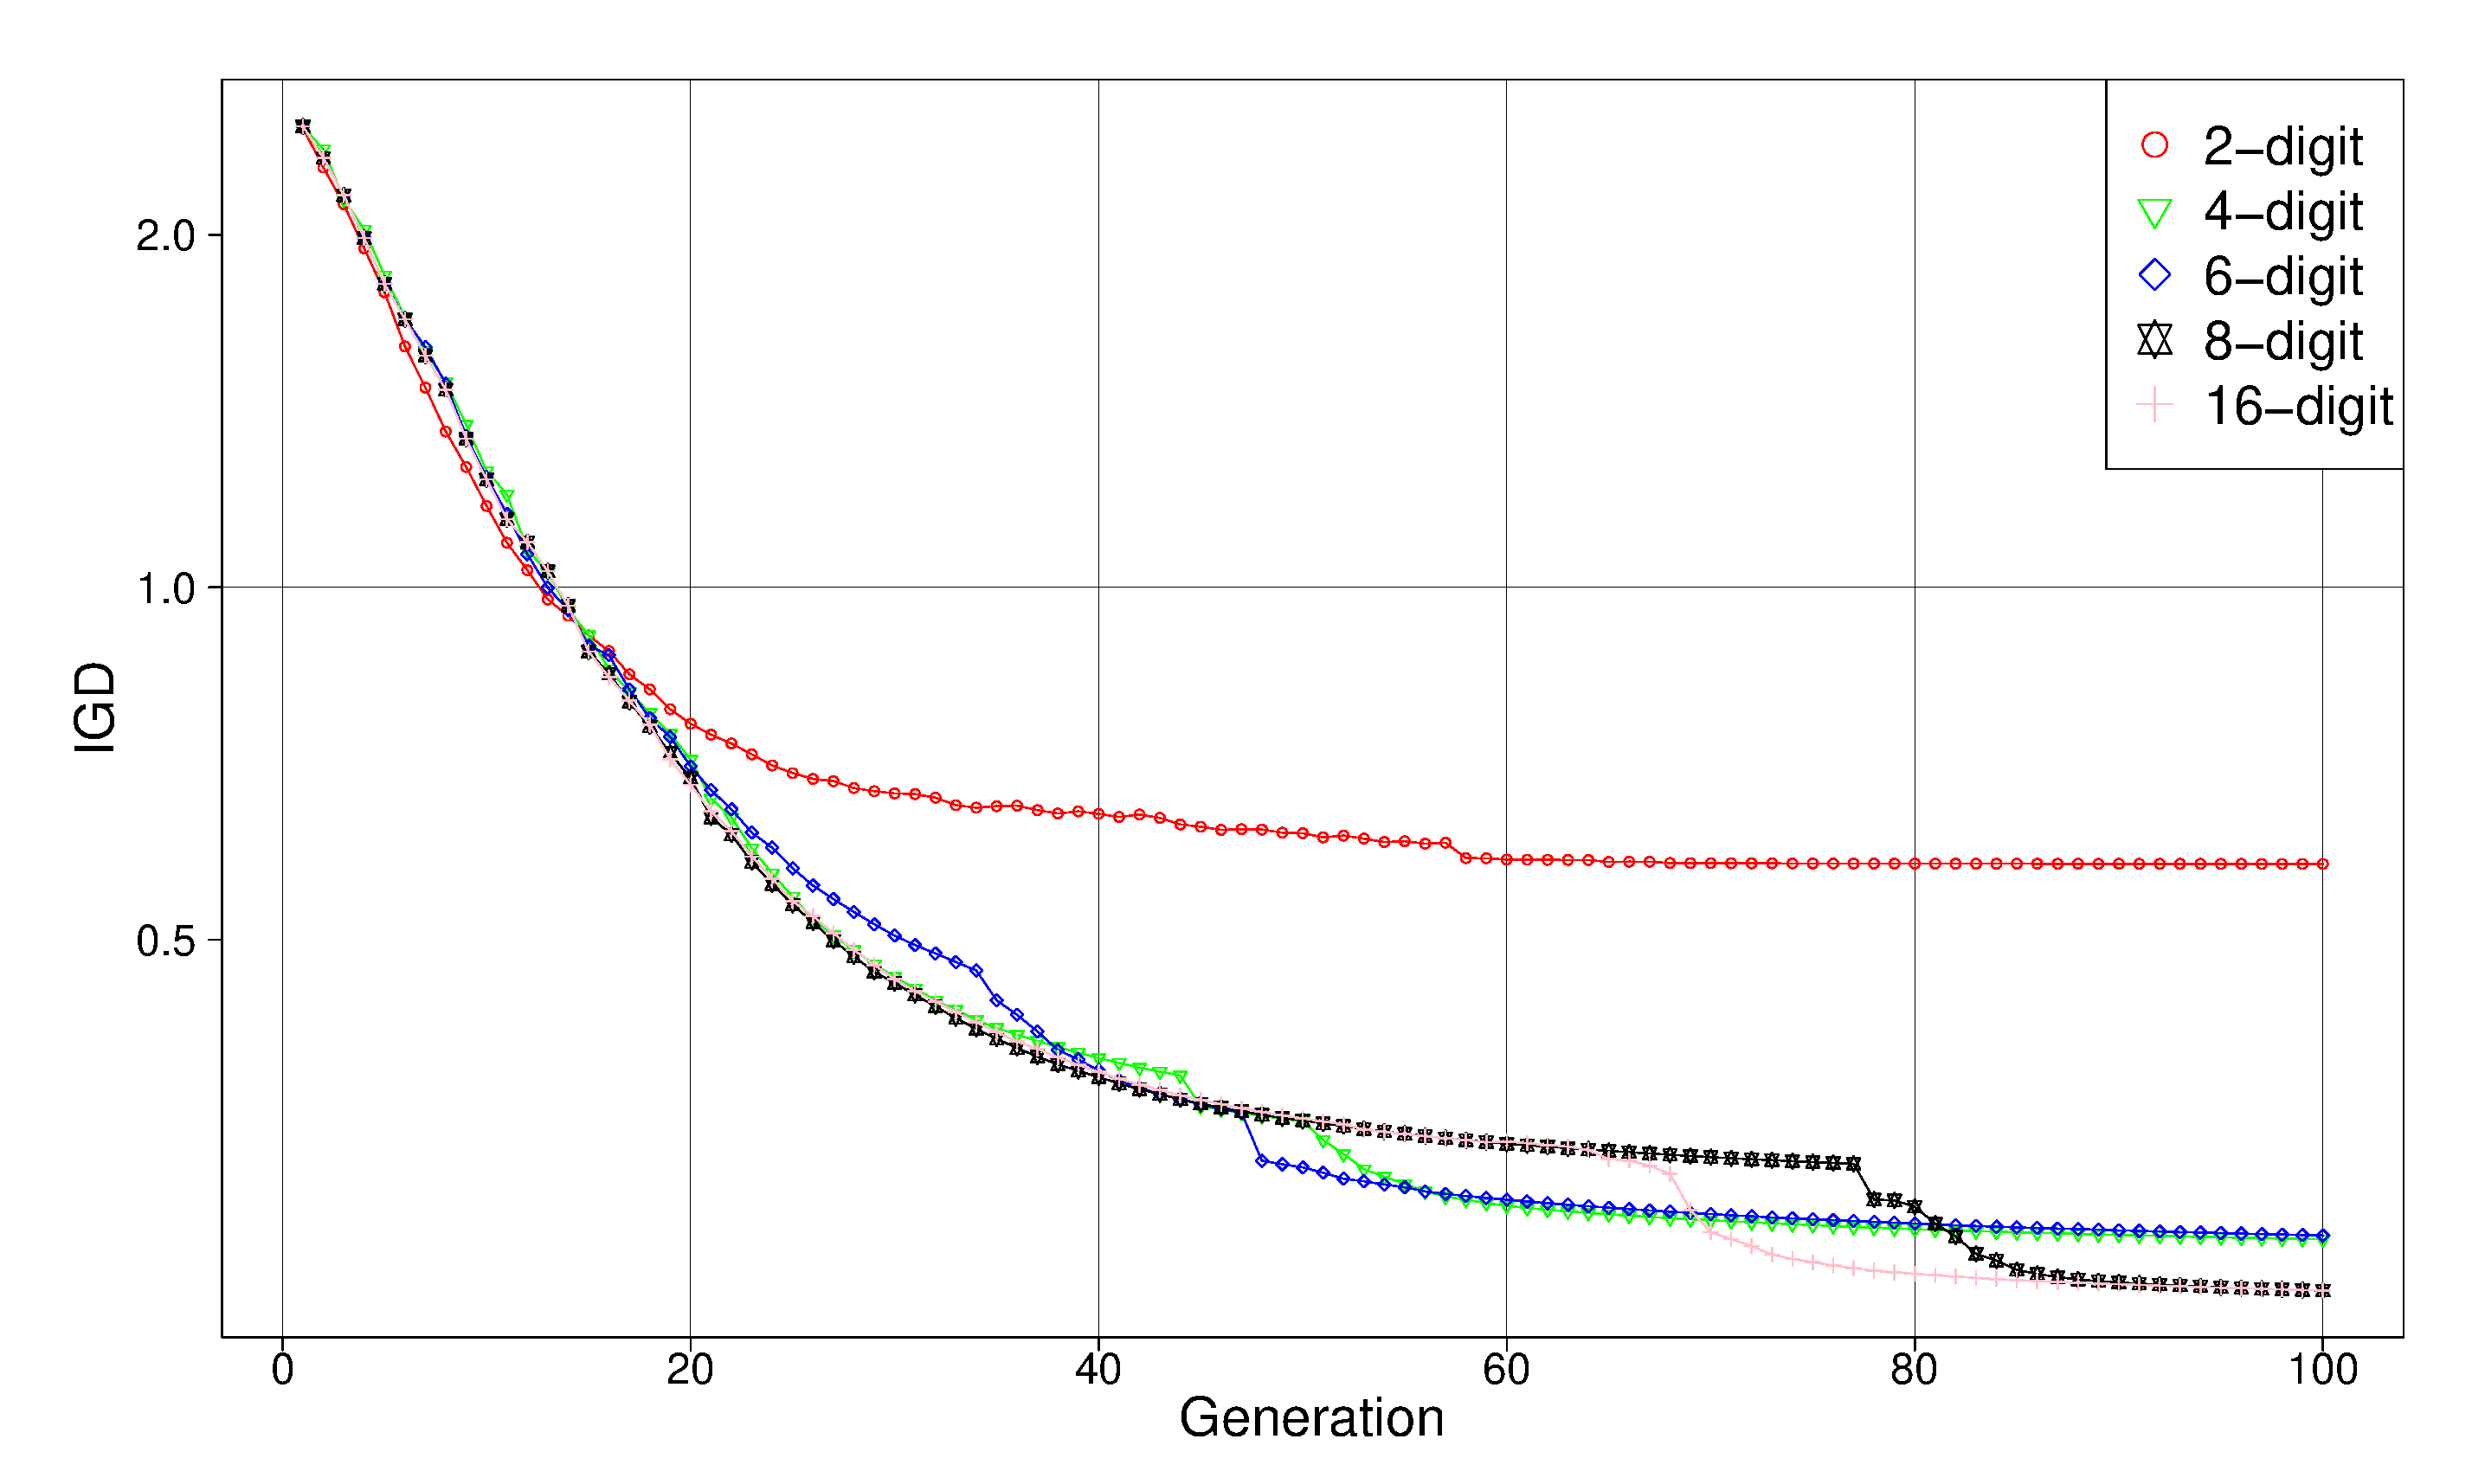
\includegraphics[width=1\linewidth]{../figures/DTLZ4_IGD.eps}
%\setlength{\abovecaptionskip}{-8mm}
%\setlength{\belowcaptionskip}{-5mm}
%\caption{a}
\begin{center}
{\footnotesize (c) DTLZ4}
\end{center}
\end{minipage}
\end{tabular}
\caption{DTLZ2-4におけるIGDの推移(NSGA-II)}
\label{fig:igd}
%\setlength\textfloatsep{-5mm}
\end{figure*}

%\vspace{-0.2in}

\begin{figure*}[htbp]
\begin{tabular}{cc}
\begin{minipage}{0.32\hsize}
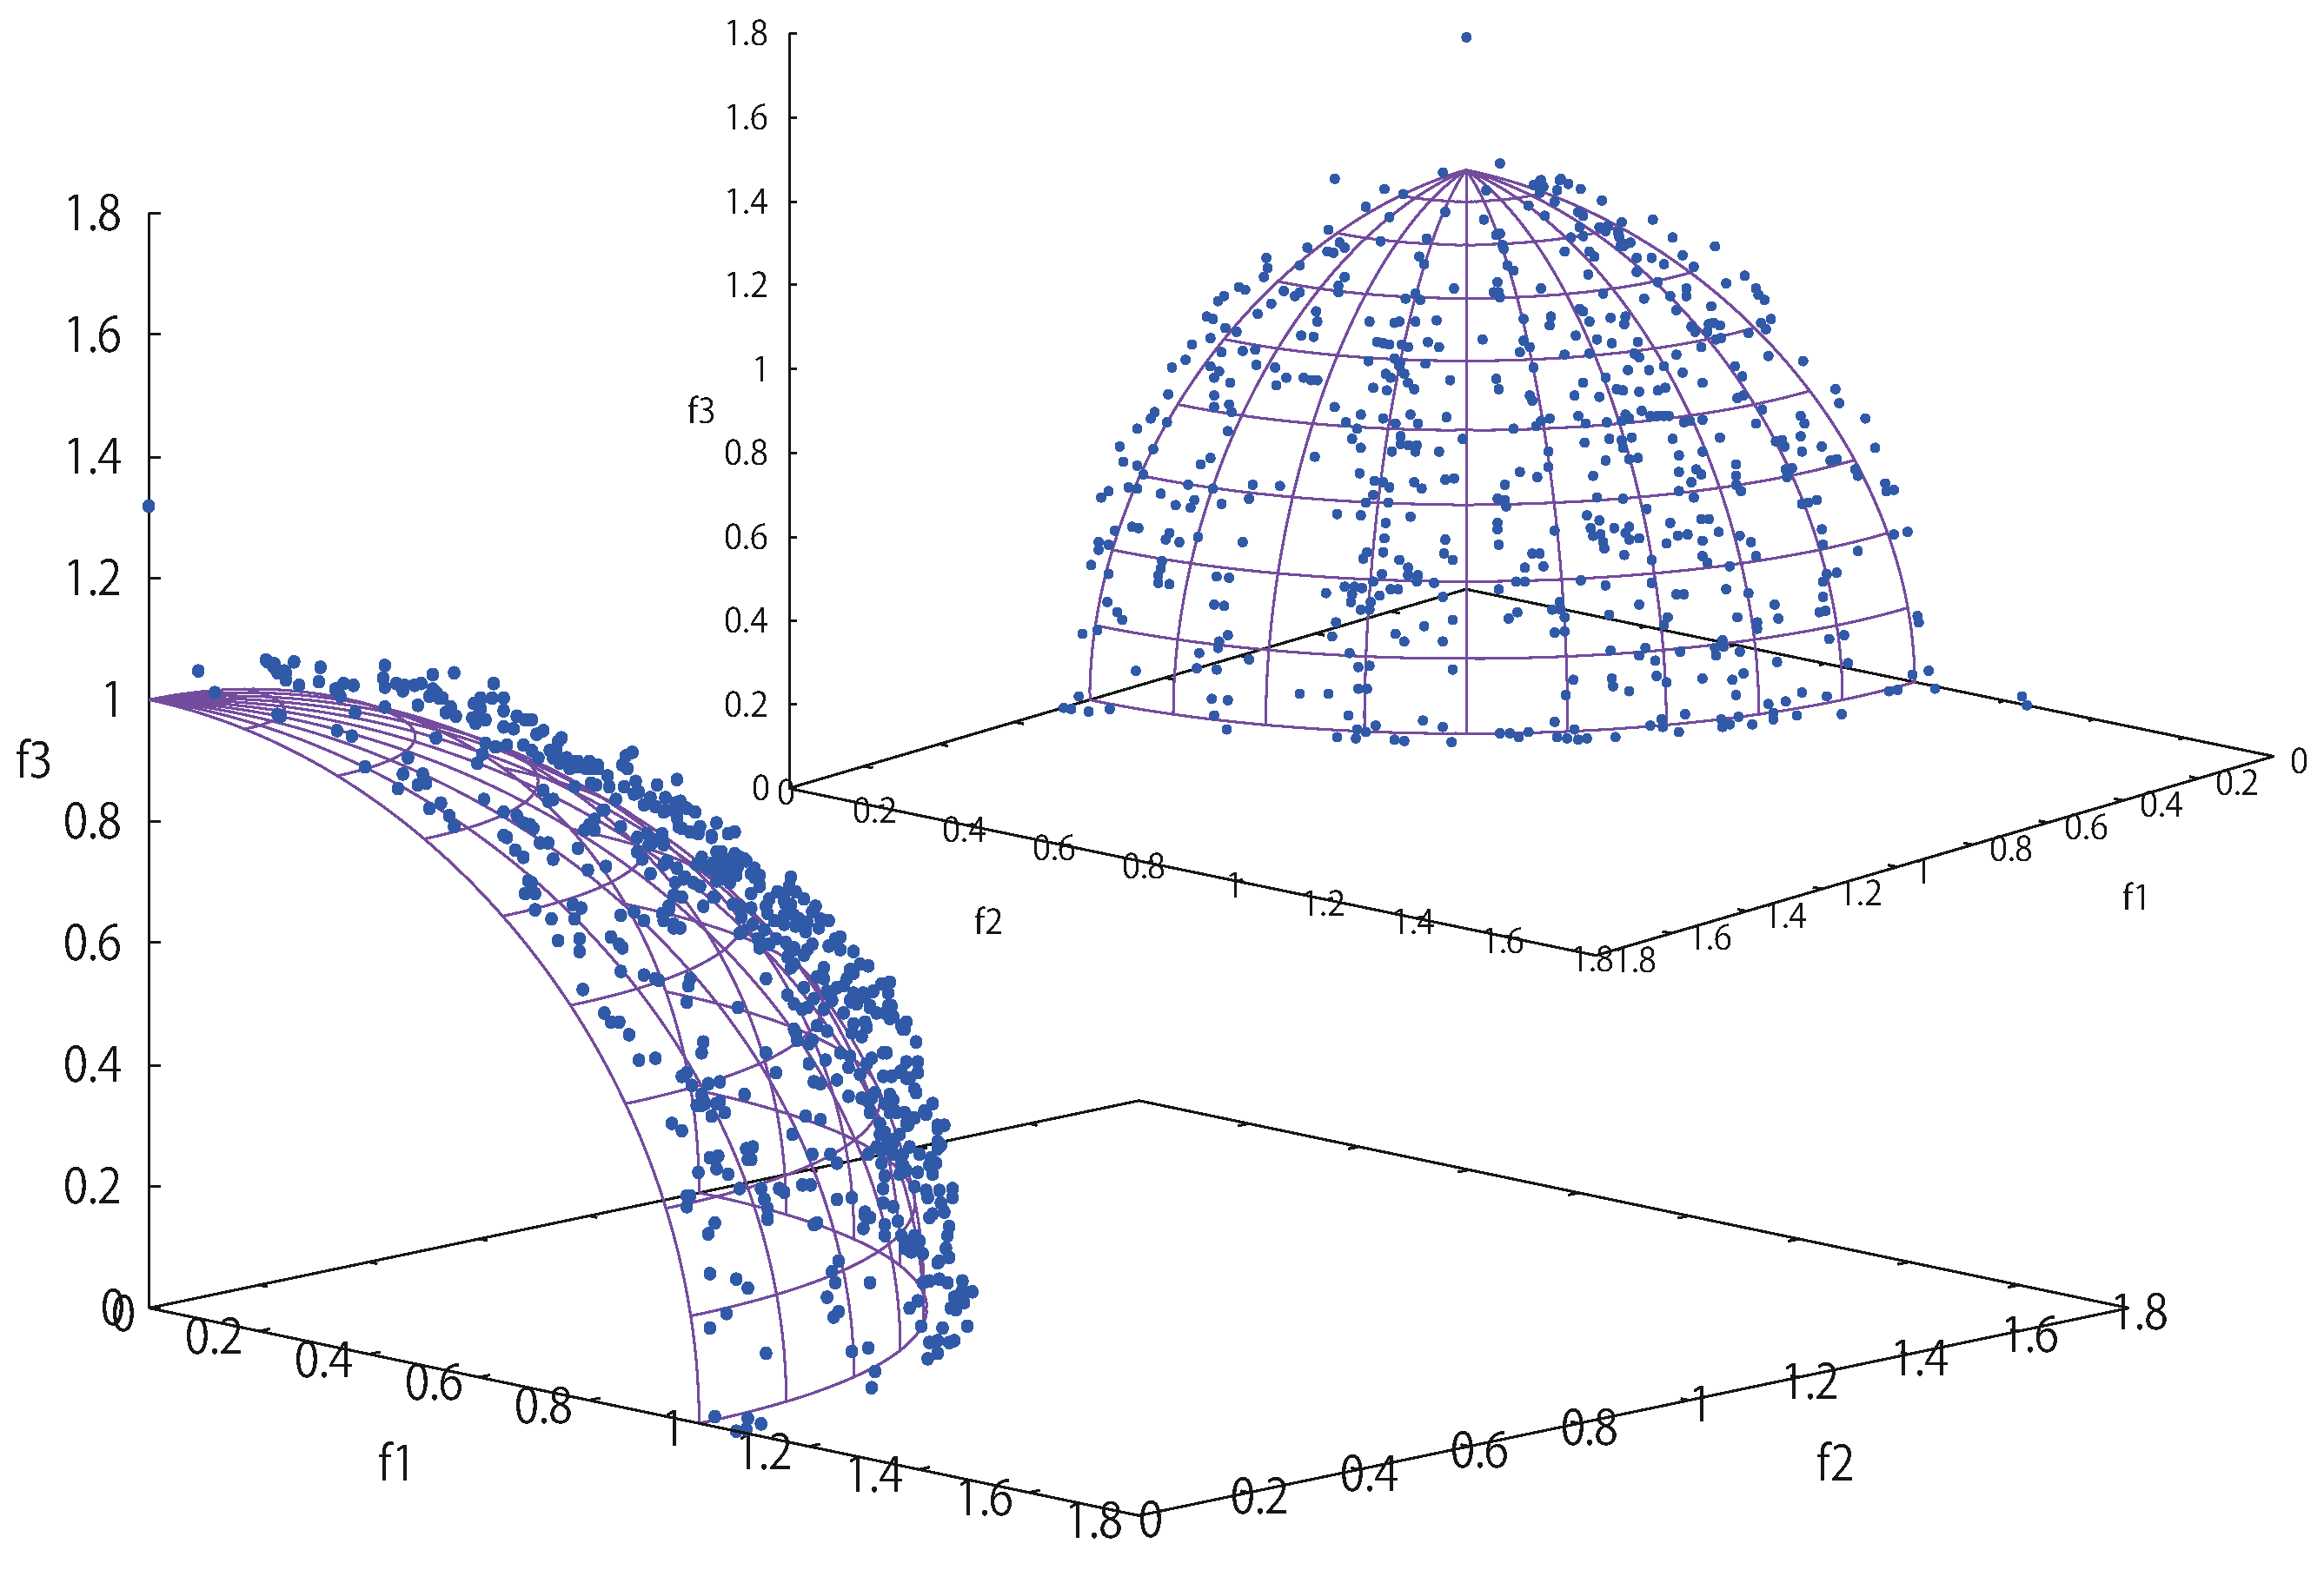
\includegraphics[width=1\linewidth]{../figures/DTLZ2digi2_double.pdf}
%\setlength{\abovecaptionskip}{-8mm}
%\setlength{\belowcaptionskip}{-5mm}
%\caption{a}
\begin{center}
{\footnotesize (a) 2-digit}
\end{center}
\end{minipage}
%\hspace{-1mm}
\begin{minipage}{0.32\hsize}
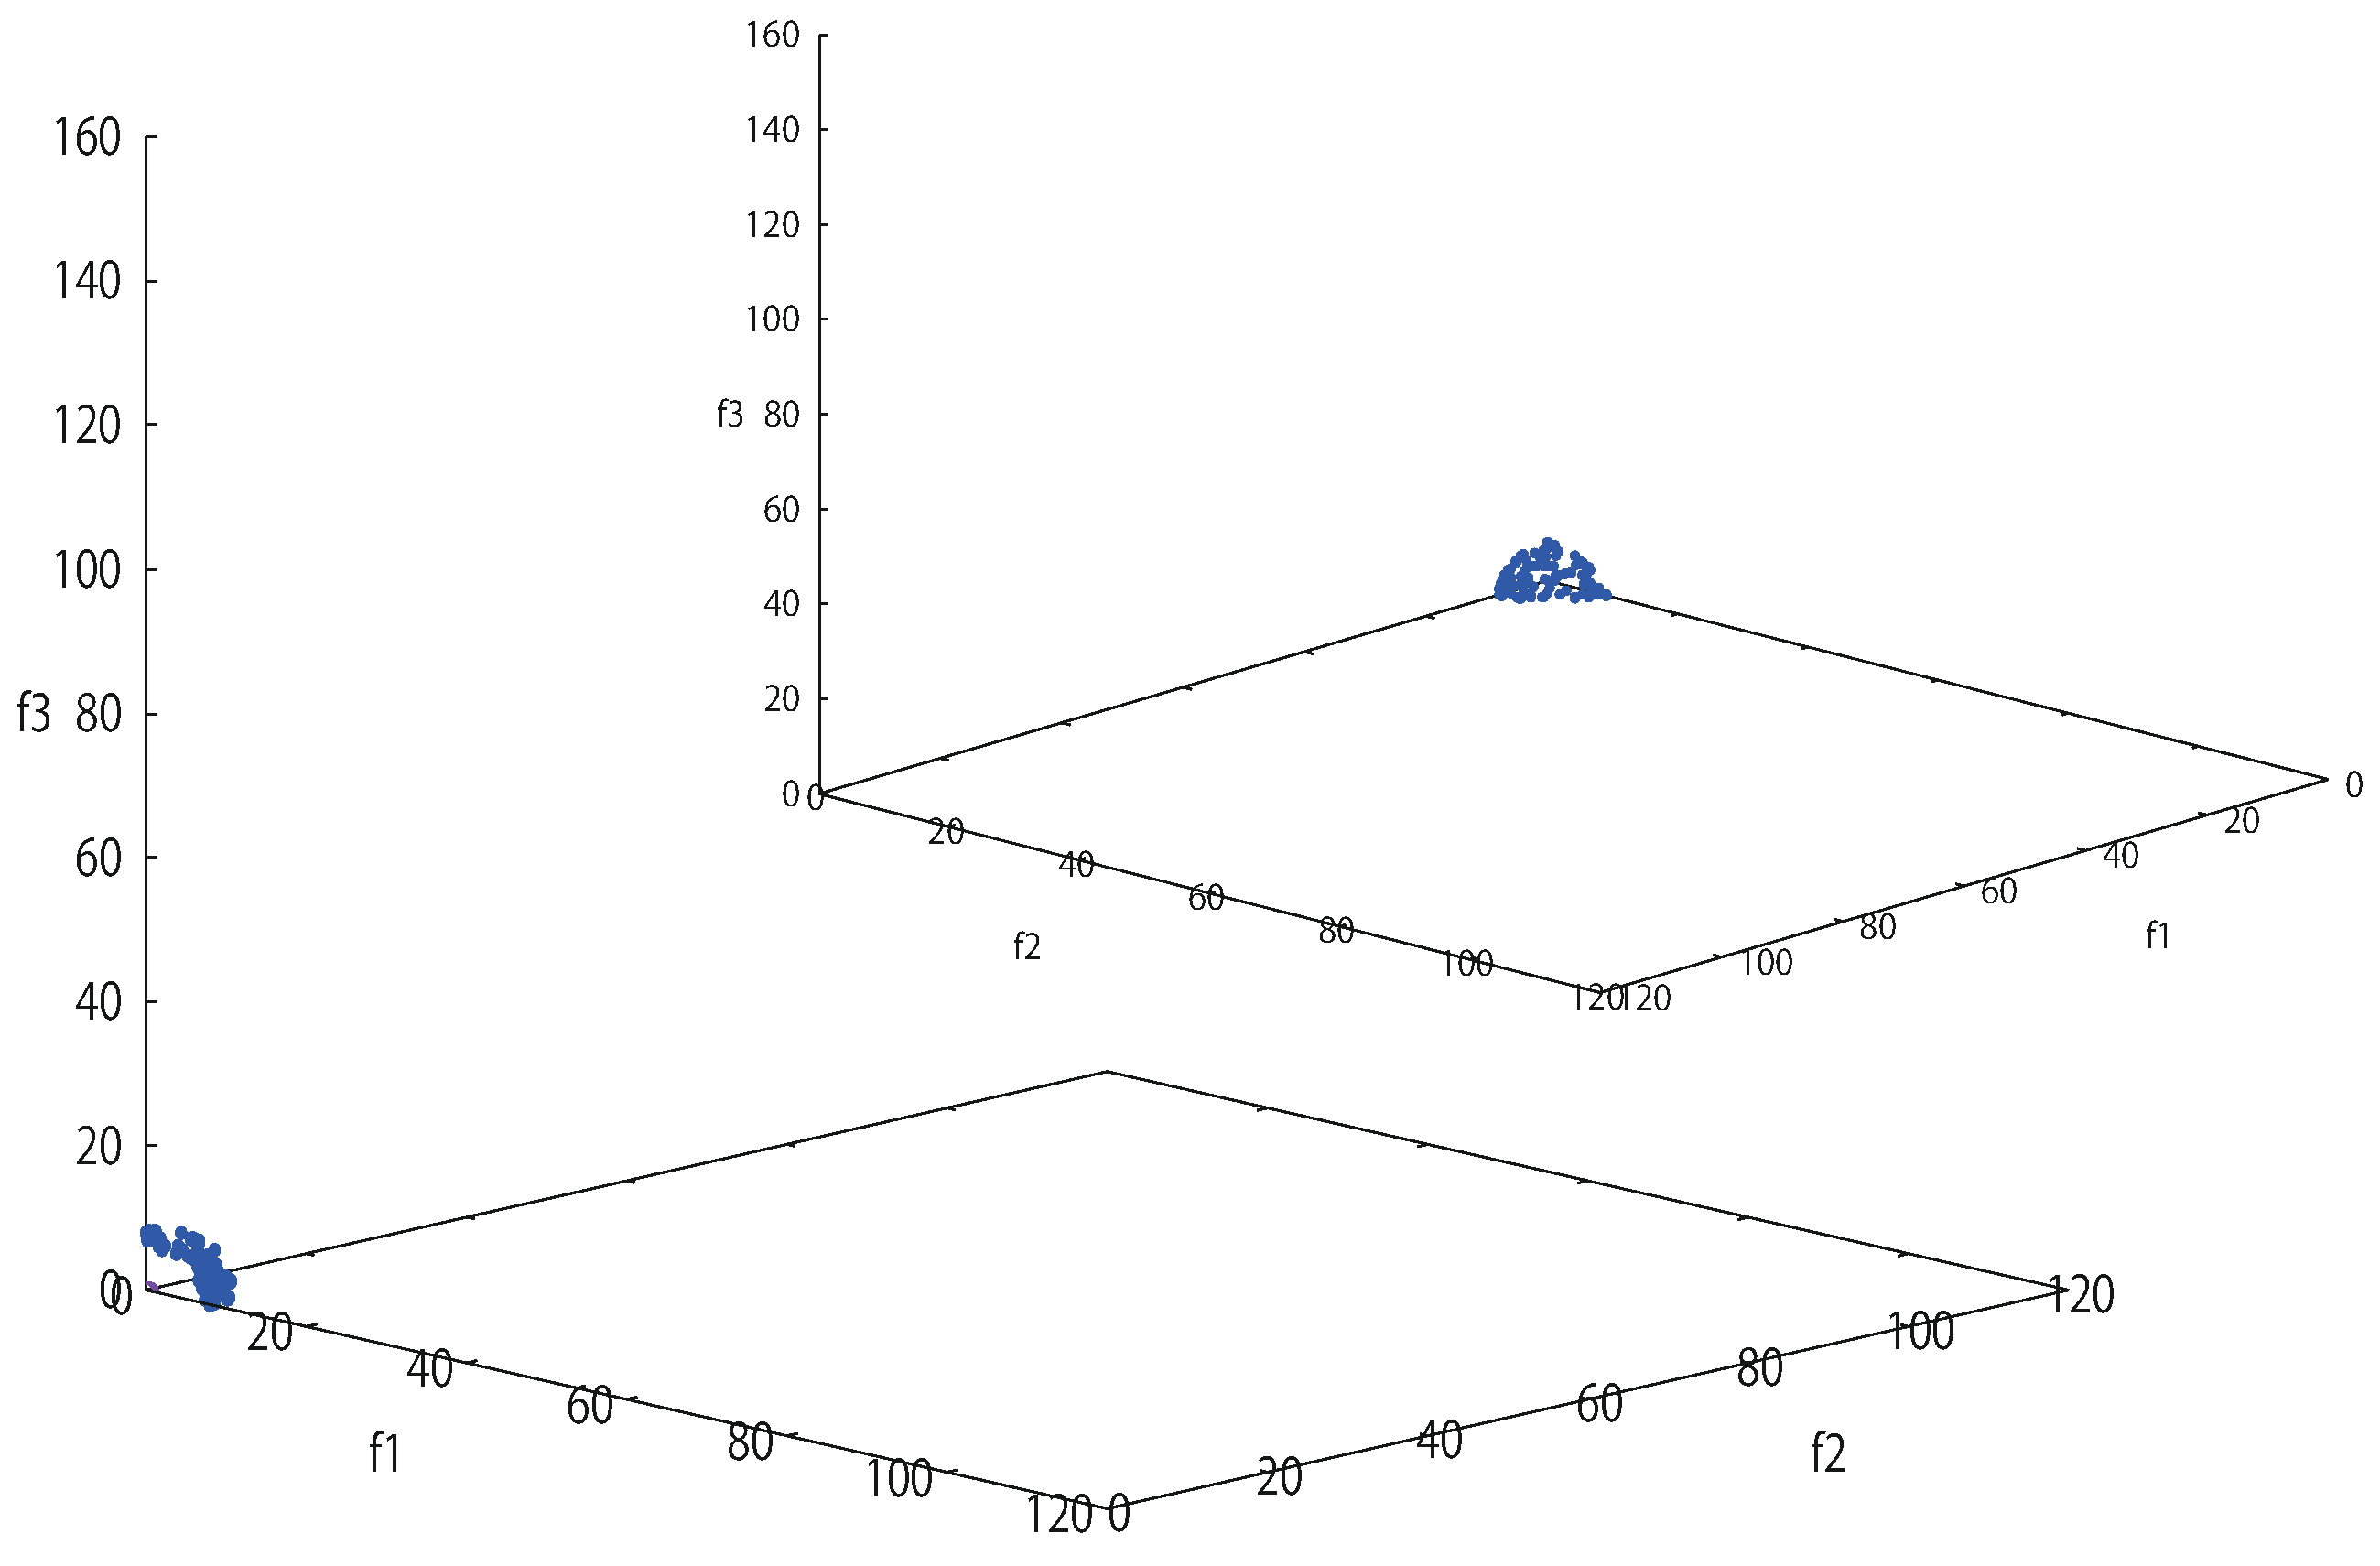
\includegraphics[width=1\linewidth]{../figures/DTLZ3digi2_double.pdf}
%\setlength{\abovecaptionskip}{-8mm}
%\setlength{\belowcaptionskip}{-5mm}
%\caption{a}
\begin{center}
{\footnotesize (a) 2-digit}
\end{center}
\end{minipage}
\begin{minipage}{0.32\hsize}
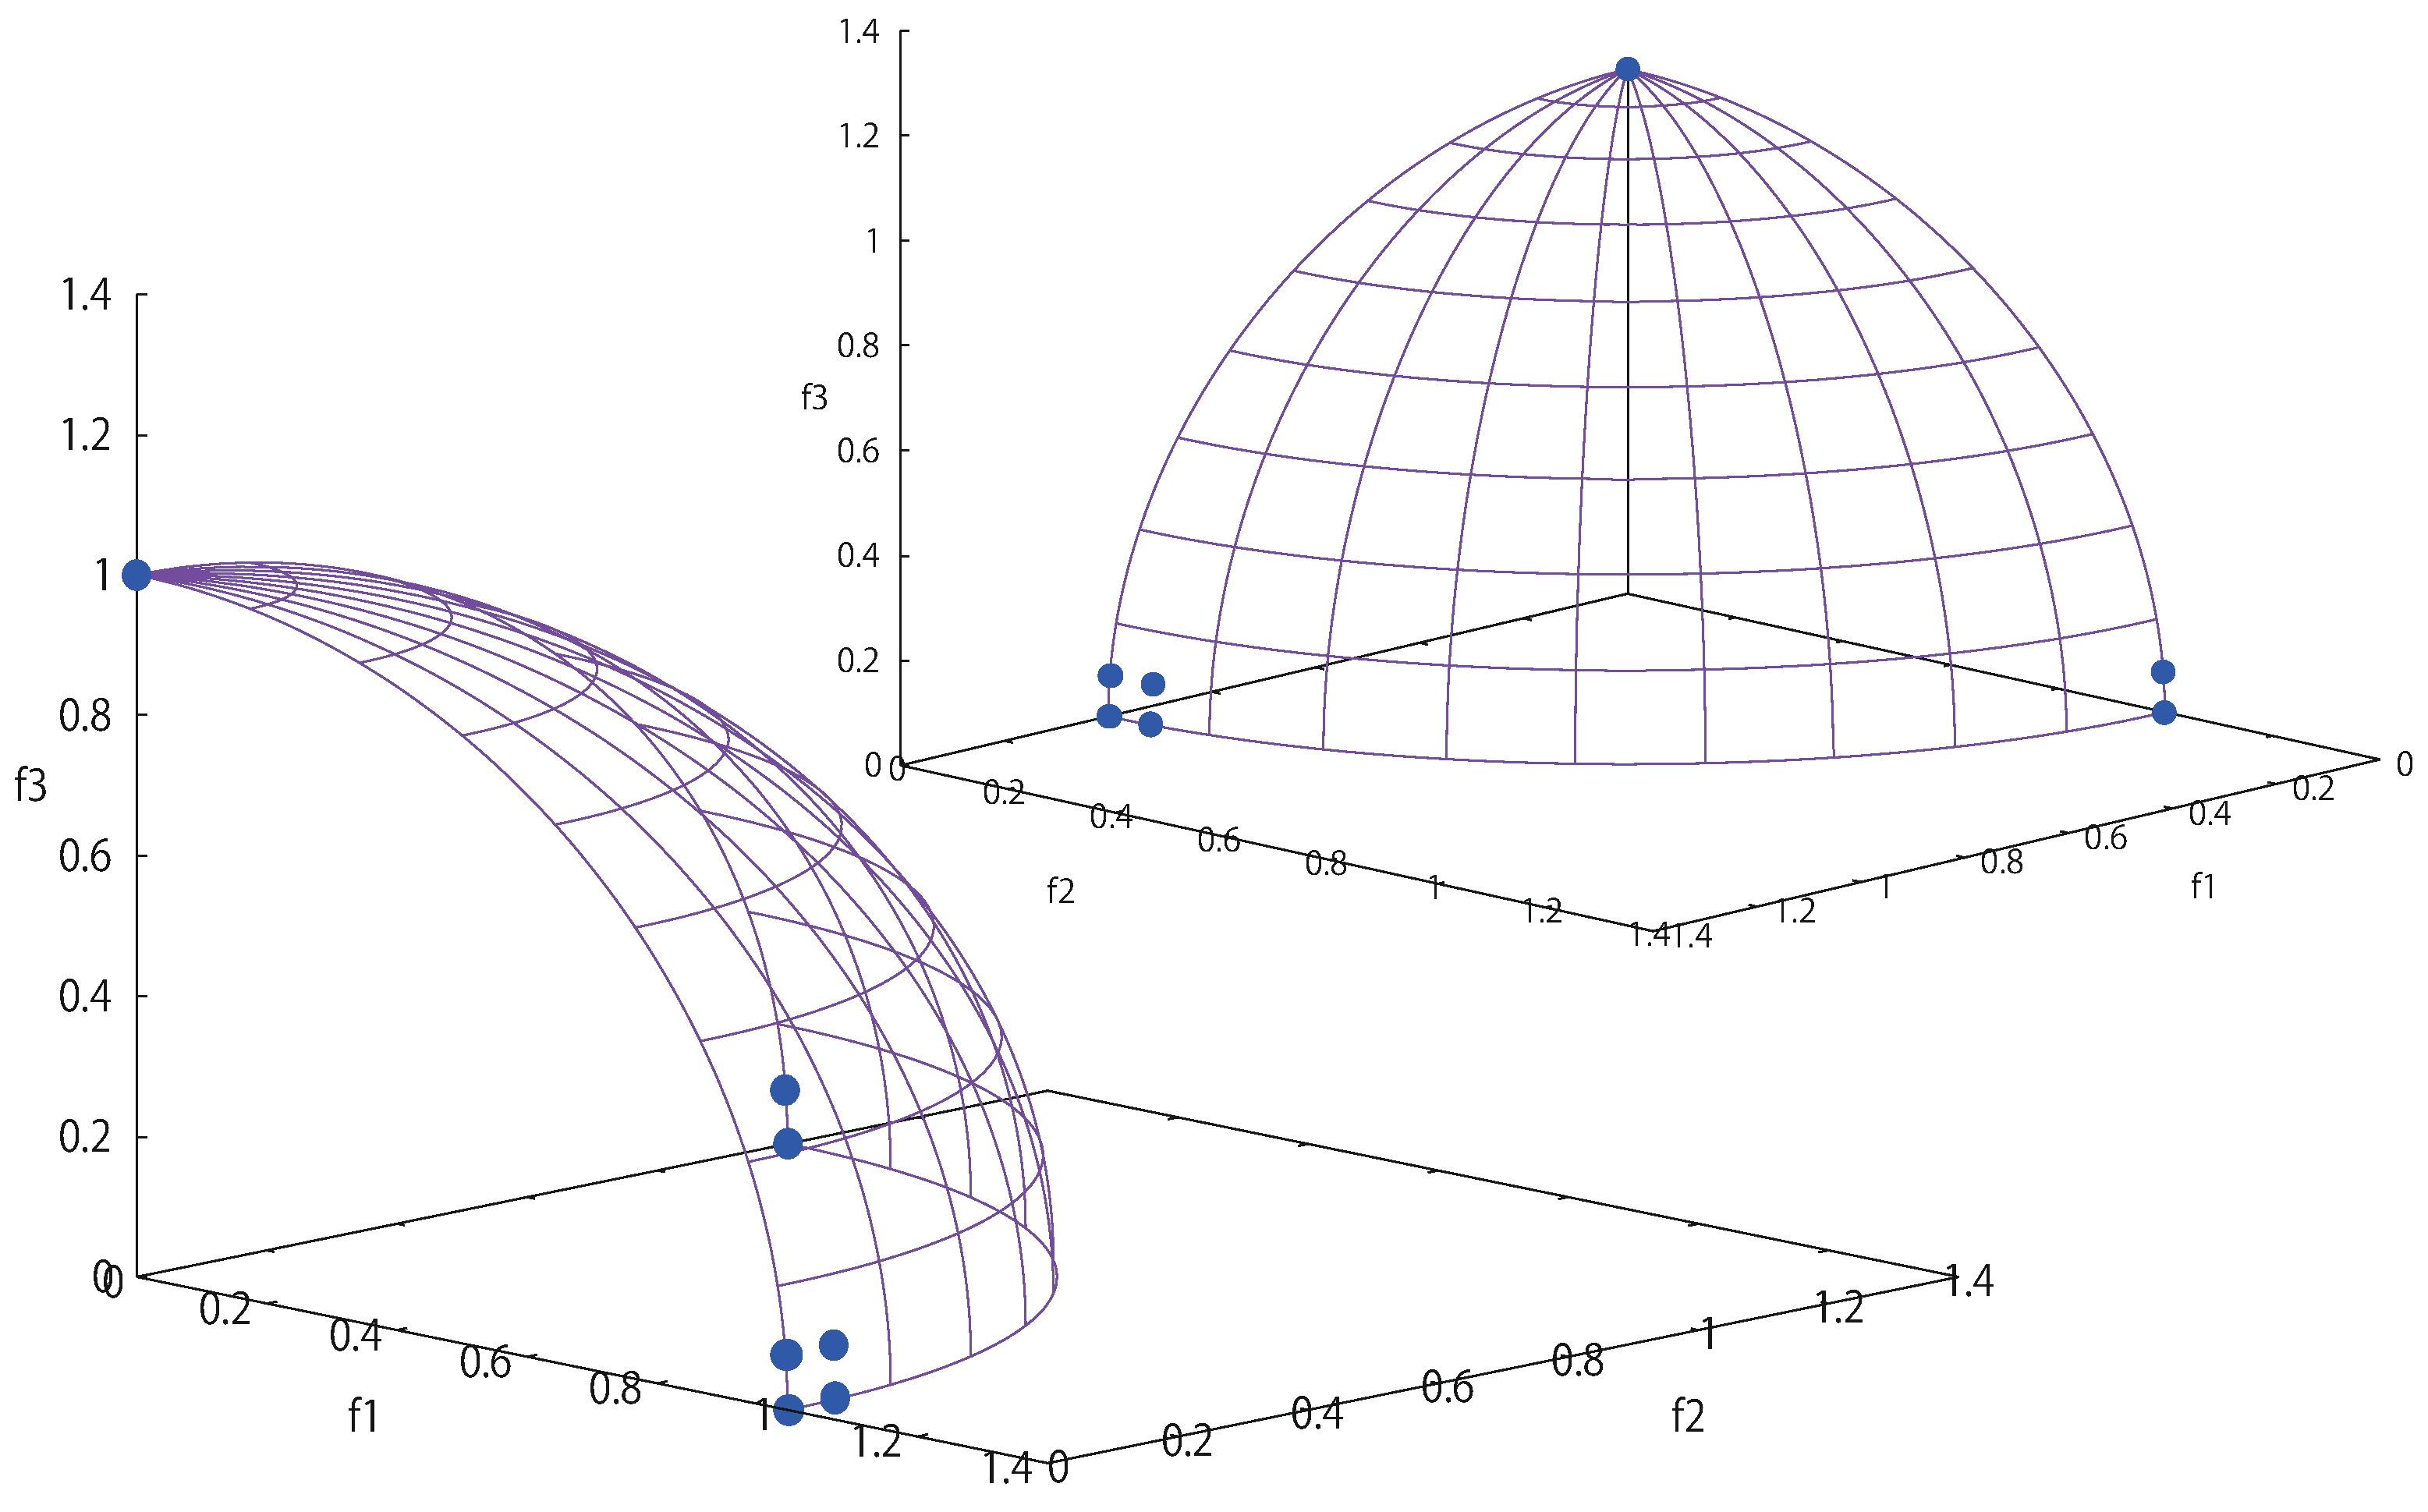
\includegraphics[width=1\linewidth]{../figures/DTLZ4_another_double.pdf}
%\setlength{\abovecaptionskip}{-8mm}
%\setlength{\belowcaptionskip}{-5mm}
%\caption{a}
\begin{center}
{\footnotesize (a) 2-digit}
\end{center}
\end{minipage}
\end{tabular}
%\caption{IGD transition and plots of final non-dominated individuals in the case of using 2- and 16-digit on DTLZ4.}
\label{fig:dtlz4}
%\setlength\textfloatsep{-5mm}
\end{figure*}



\begin{figure*}[!hb]
\begin{tabular}{cc}
\begin{minipage}{0.32\hsize}
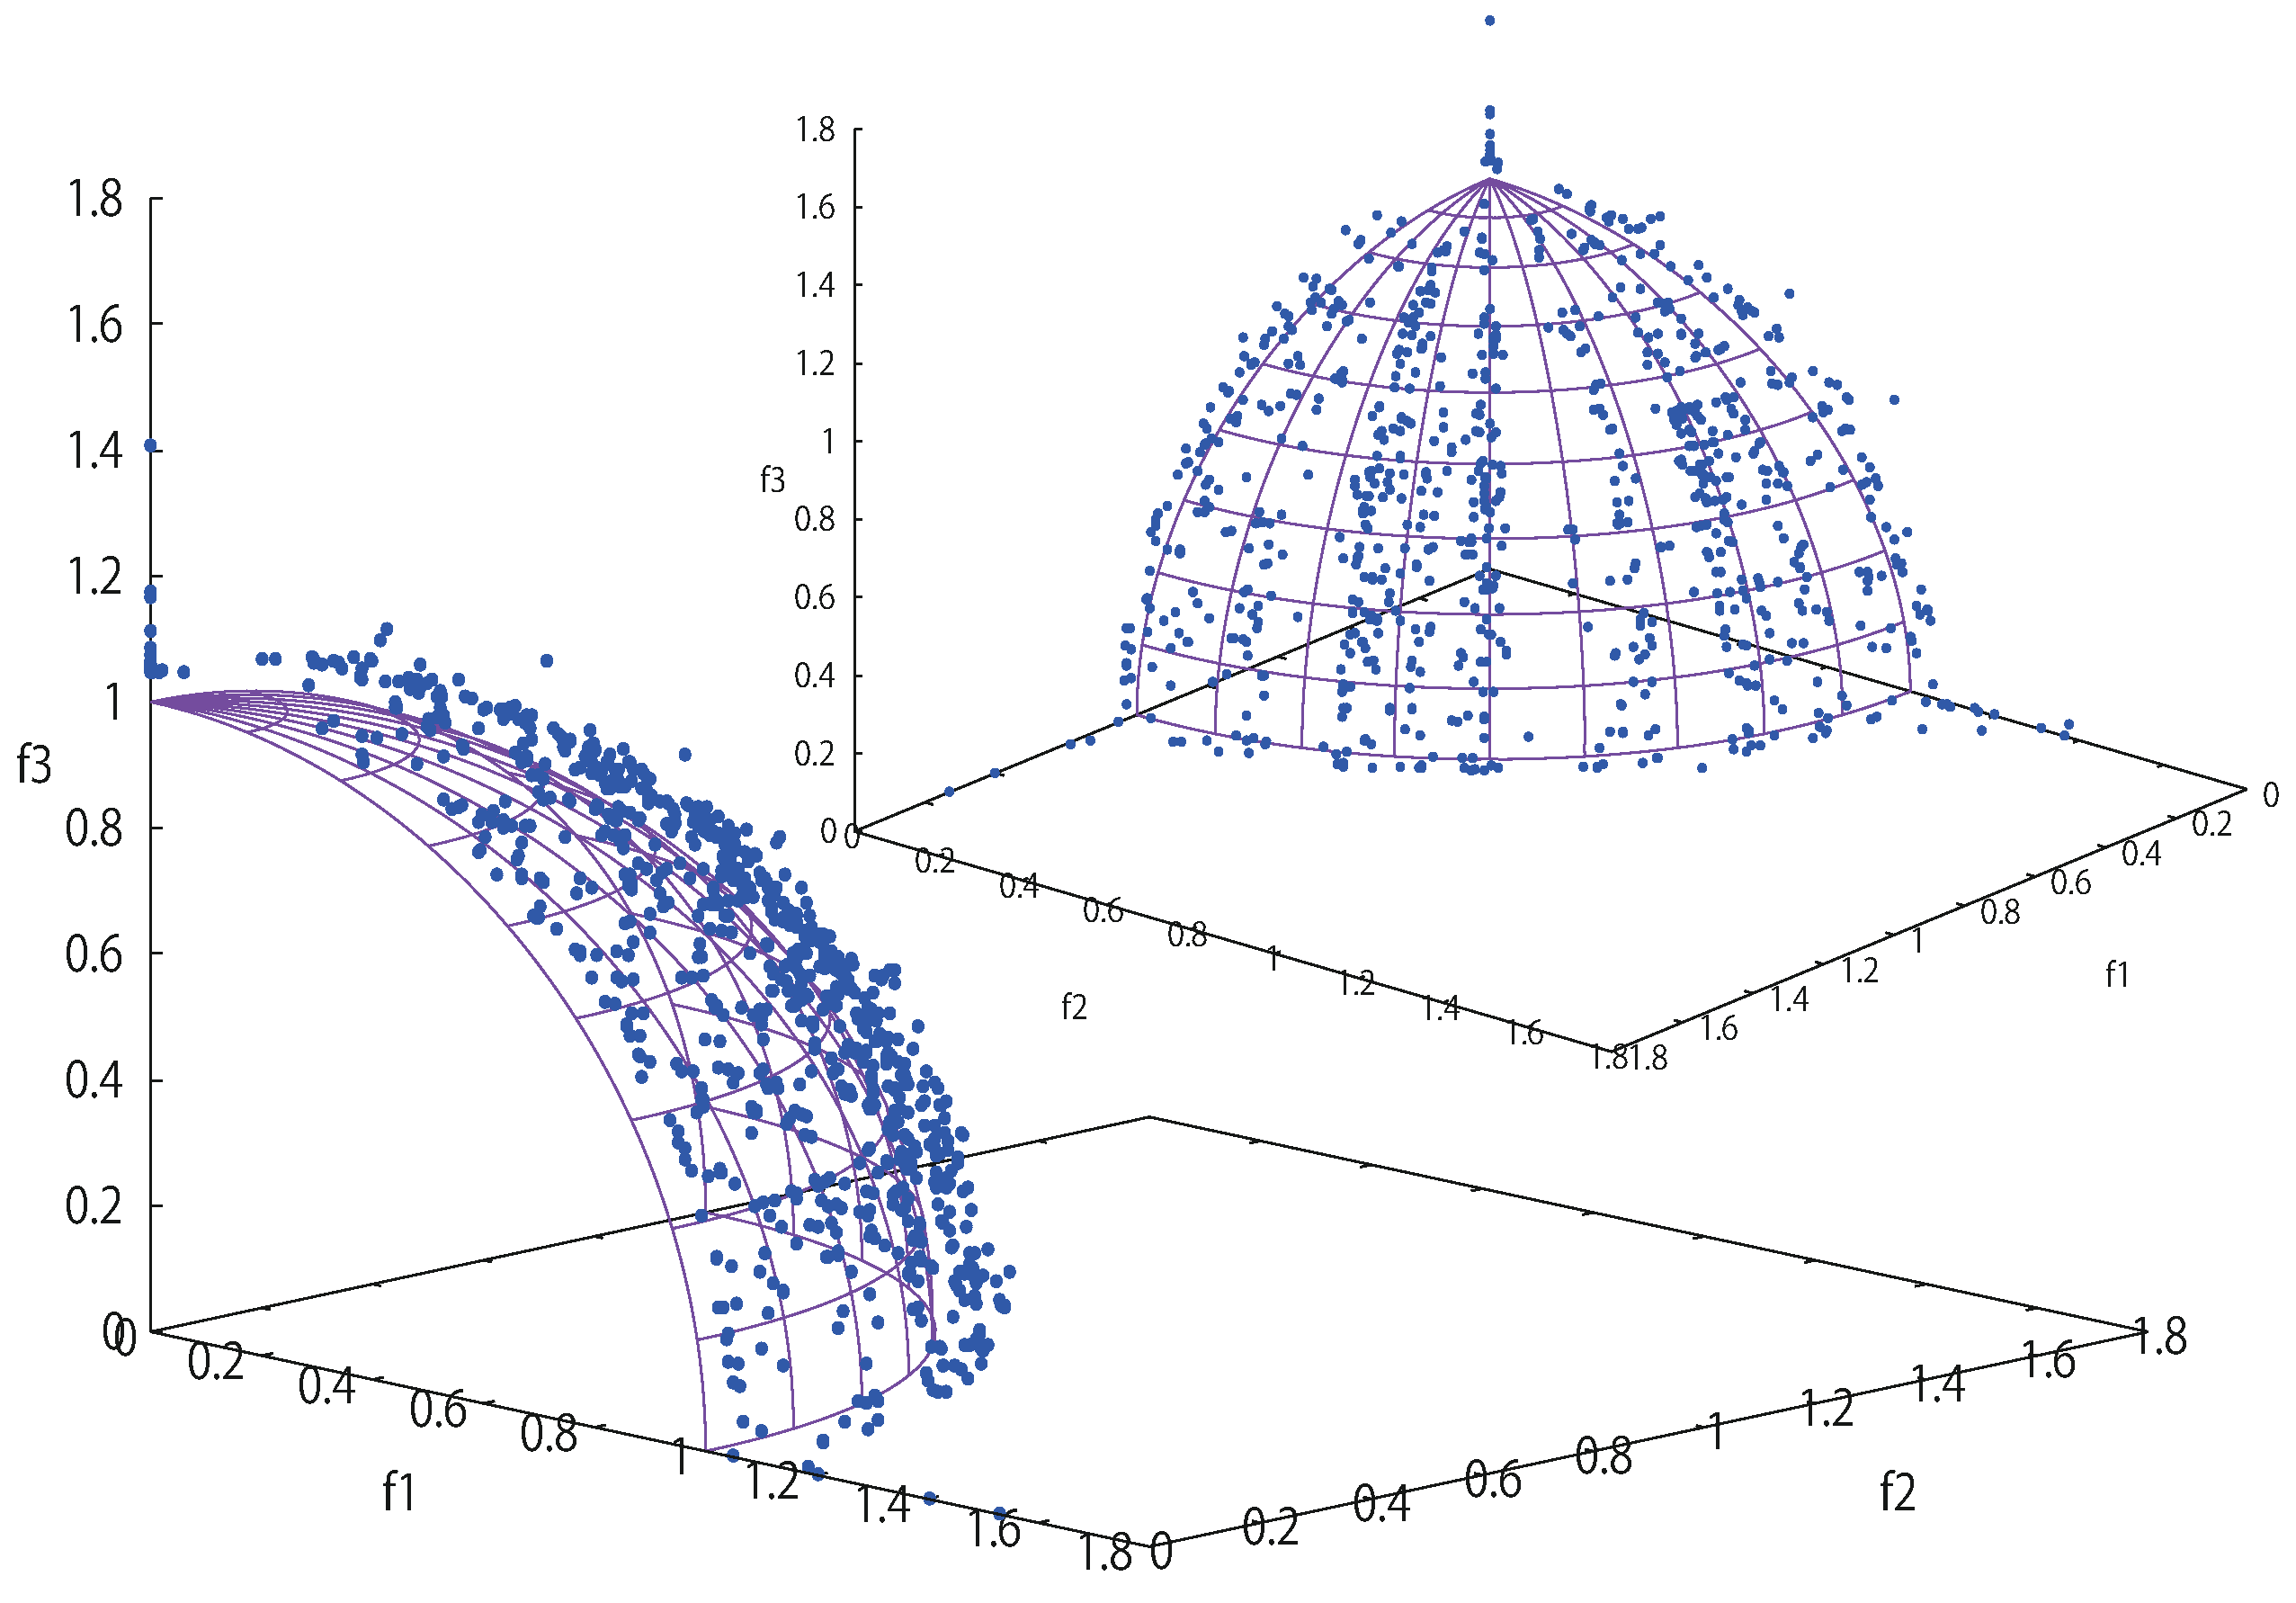
\includegraphics[width=1\linewidth]{../figures/DTLZ2digi16_double.pdf}
%\setlength{\abovecaptionskip}{-8mm}
%\setlength{\belowcaptionskip}{-5mm}
%\caption{a}
\centering
{\footnotesize (b) 16-digit}
\caption{DTLZ2における非劣解の分布(NSGA-II)}
\label{non_a}
\end{minipage}
%\hspace{-1mm}
\begin{minipage}{0.32\hsize}
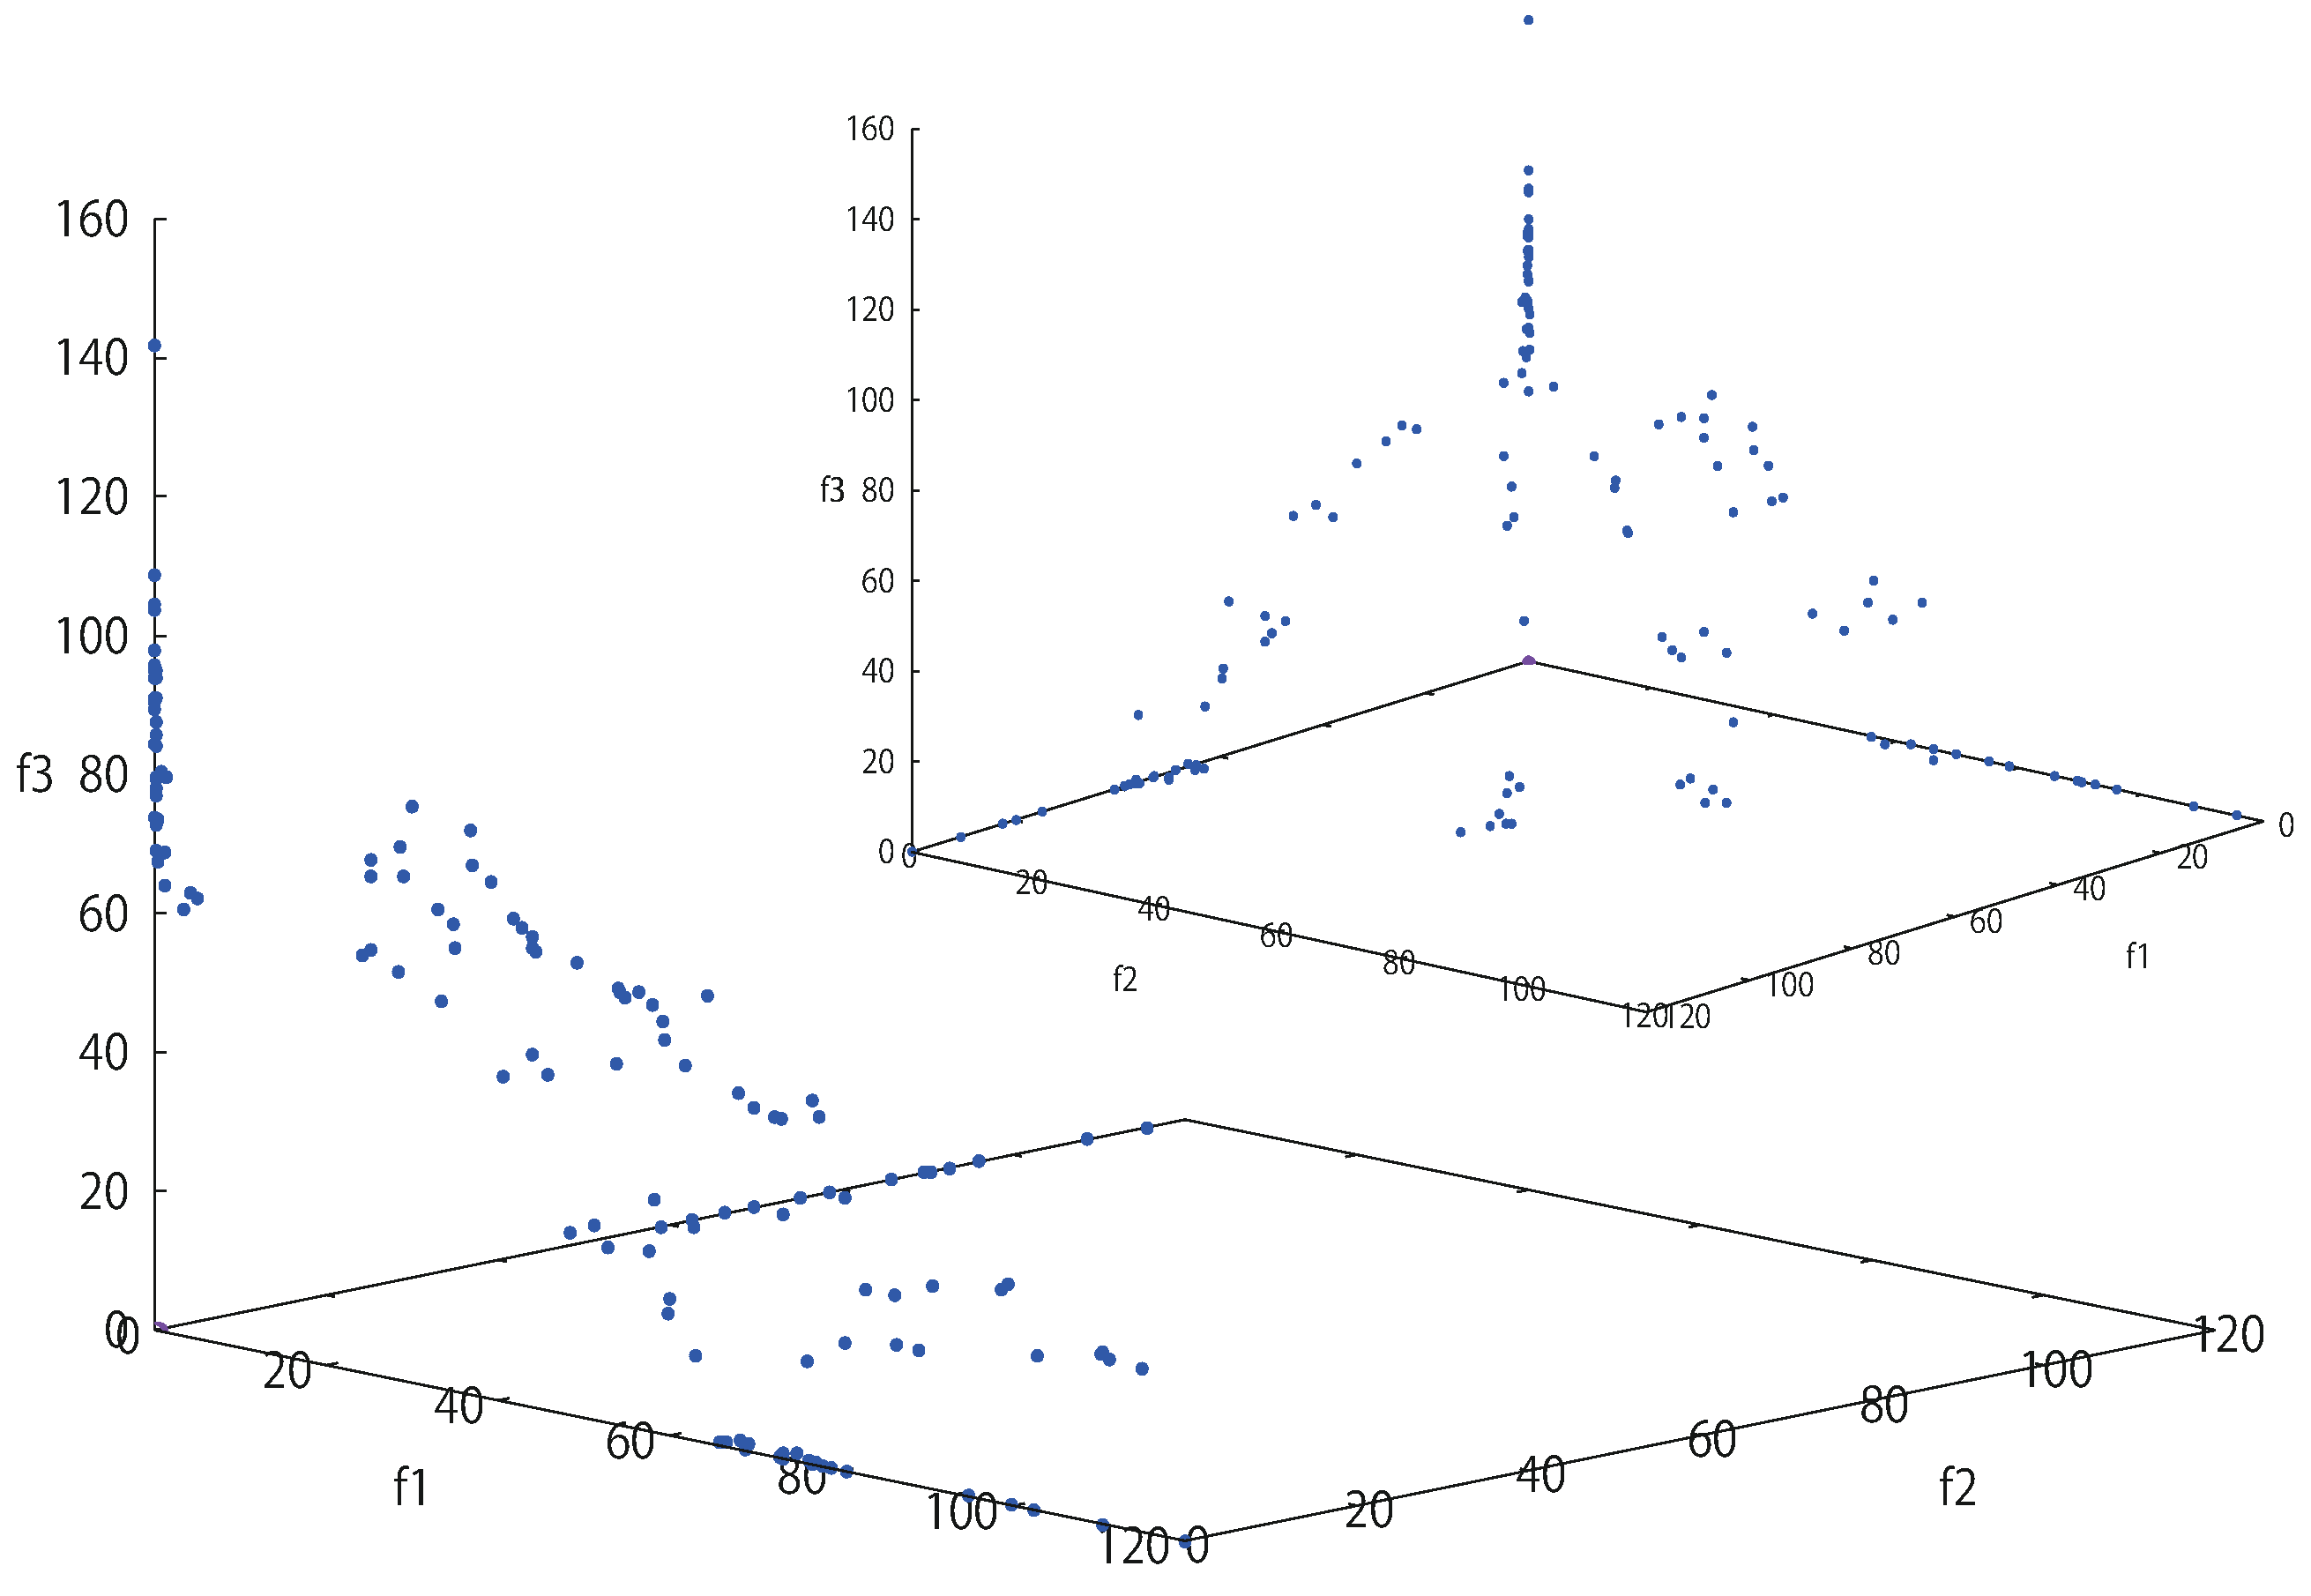
\includegraphics[width=1\linewidth]{../figures/DTLZ3digi16_double.pdf}
%\setlength{\abovecaptionskip}{-8mm}
%\setlength{\belowcaptionskip}{-5mm}
%\caption{a}
\centering
{\footnotesize (b) 16-digit}
\caption{DTLZ3における非劣解の分布(NSGA-II)}
\label{non_b}
\end{minipage}
\begin{minipage}{0.32\hsize}
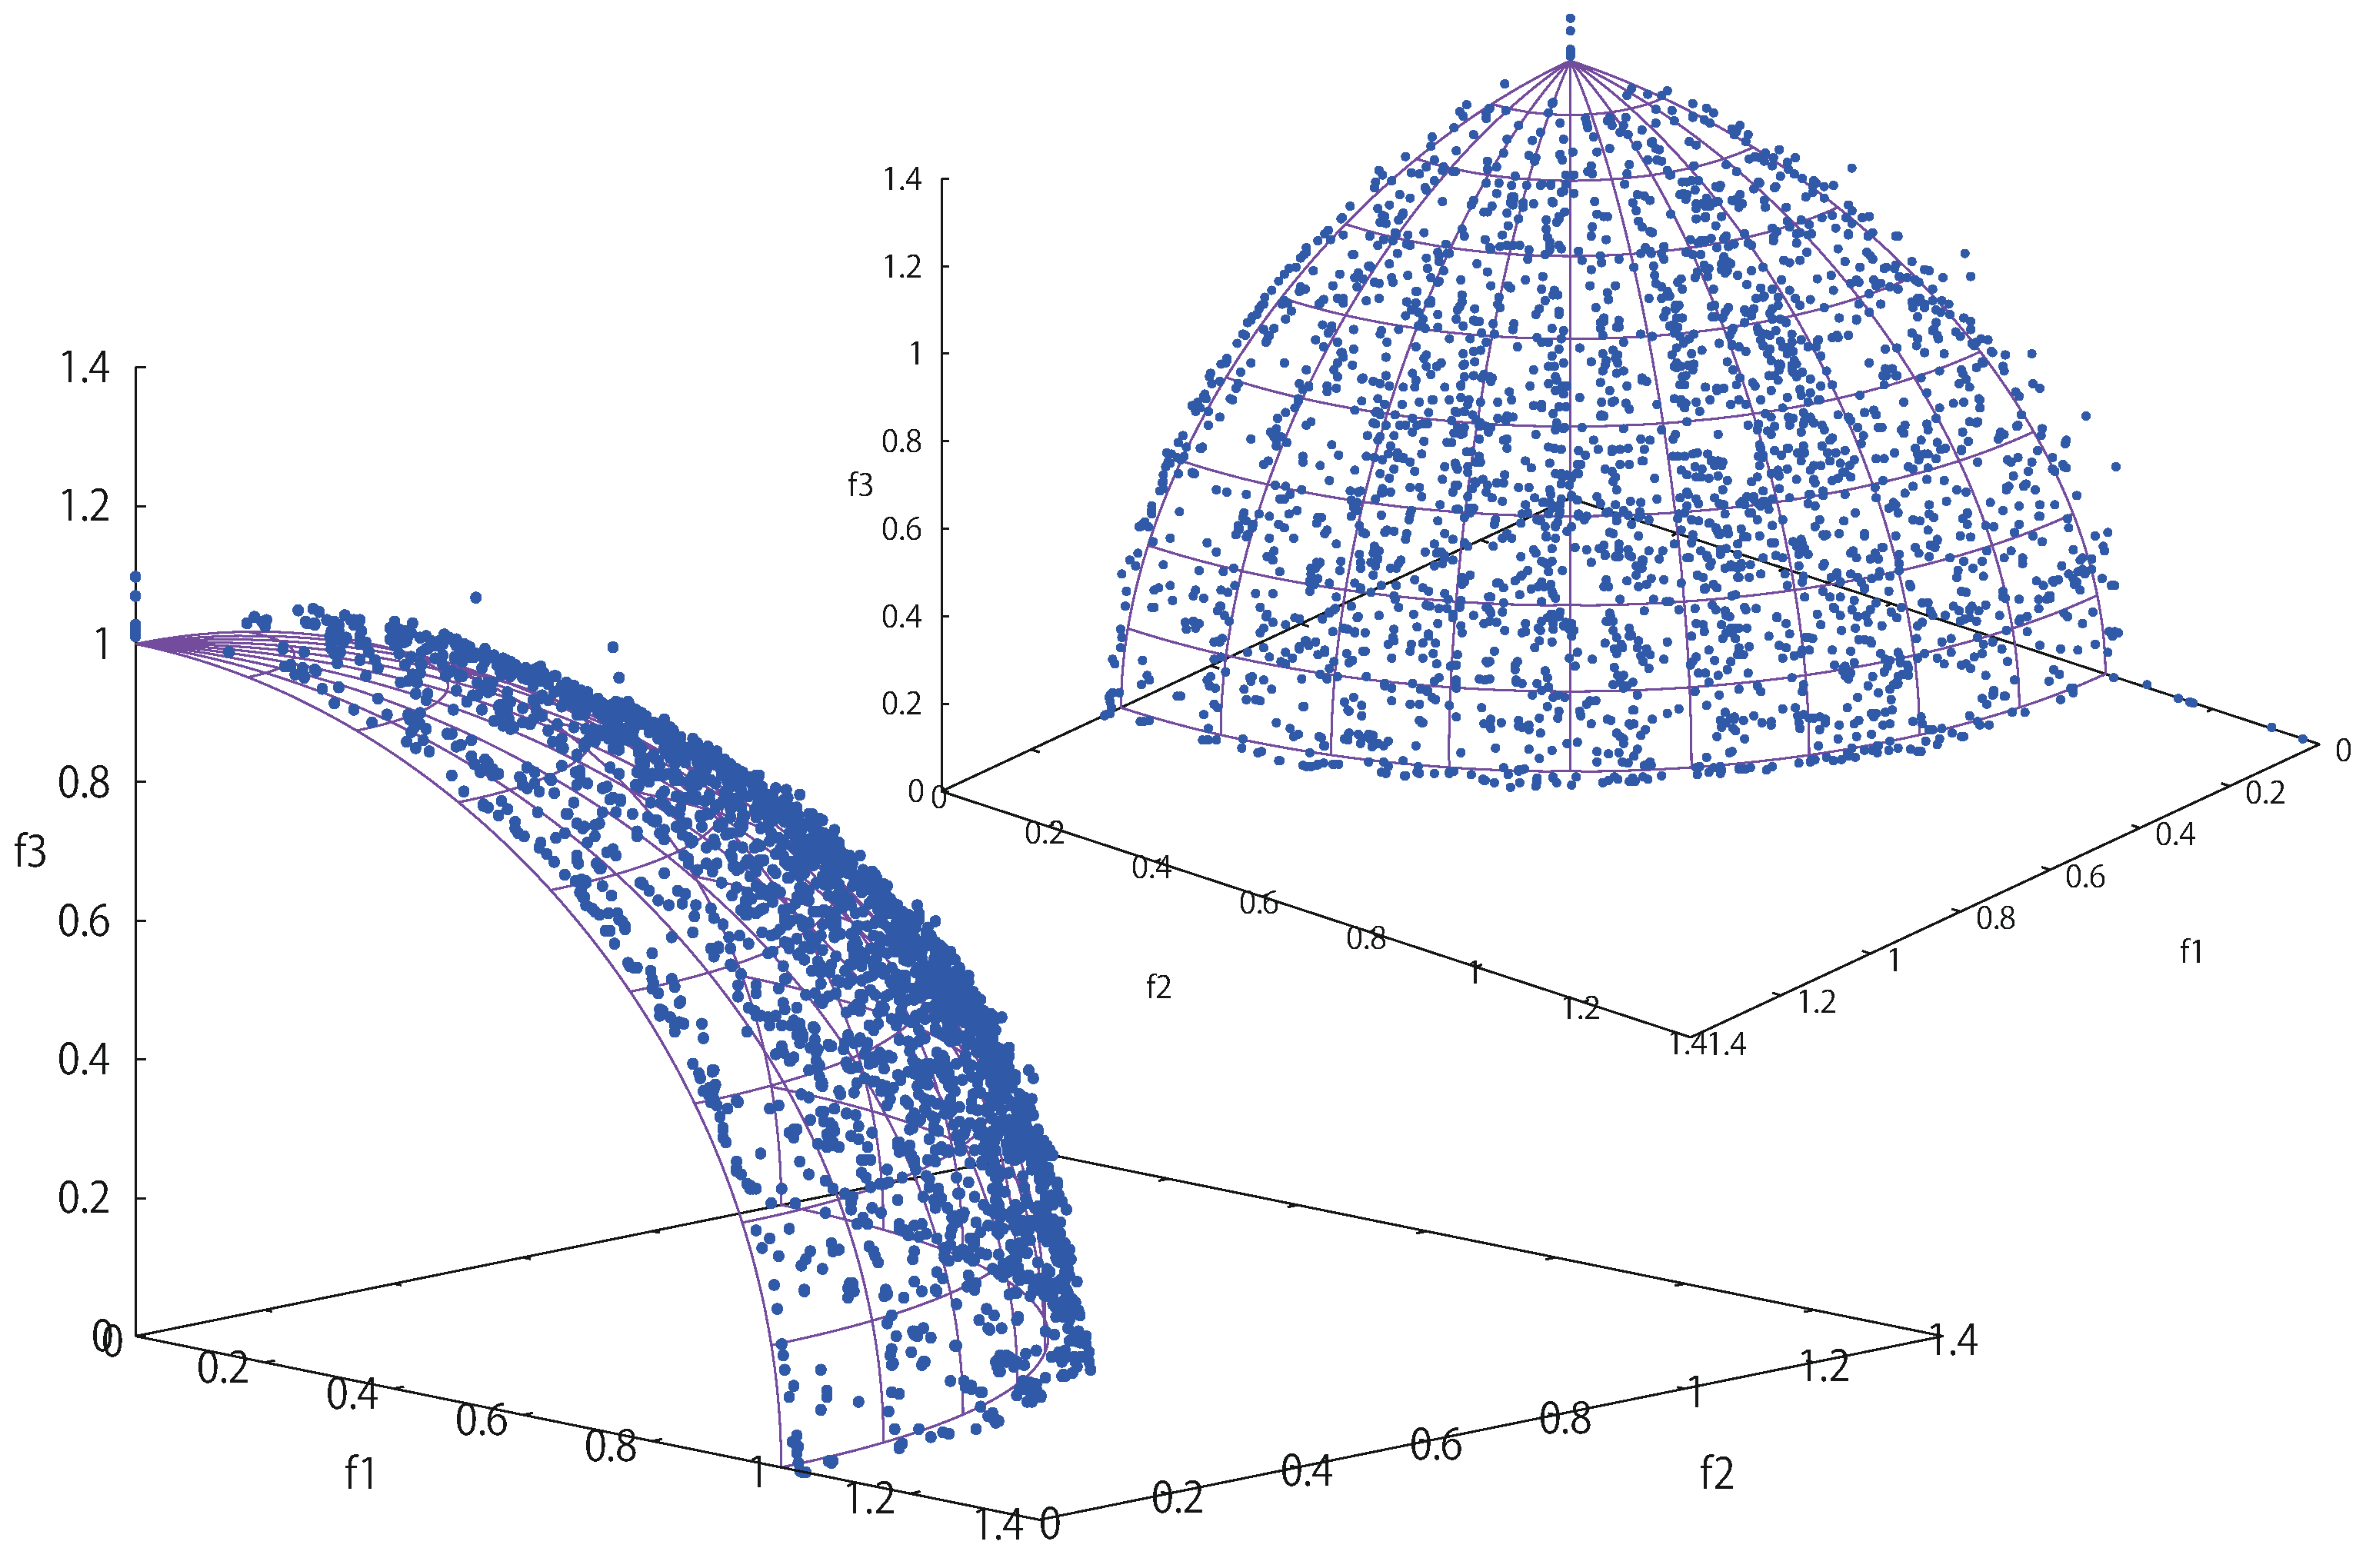
\includegraphics[width=1\linewidth]{../figures/DTLZ4_double_another.pdf}
%\setlength{\abovecaptionskip}{-8mm}
%\setlength{\belowcaptionskip}{-5mm}
%\caption{a}
\centering
{\footnotesize (b) 16-digit}
\caption{DTLZ4における非劣解の分布(NSGA-II)}
\label{non_c}
\end{minipage}
\end{tabular}
%\caption{IGD transition and plots of final non-dominated individuals in the case of using 2- and 16-digit on WFG7.}
%\label{fig:wfg7}
%\setlength\textfloatsep{-5mm}
\end{figure*}

%
\afterpage{\clearpage}

%
\quad 先行研究では,制御する桁数の違いにより進化に影響が出る原因を調べるため,さらなる検証が行われた.
離散化する粒度の違いにより結果に違いが生まれる一つの要因として交叉(SBX)と突然変異(polynominal mutation)による分布の違いが考えられる.
そこで,桁数の違いによるSBX,polynominal mutationの分布を比較した.

\quad SBXに関しては$\eta_c=30$,親個体を(0.3,0.3),(0.7,0.7)に設定し,子個体がどのように分布するか1000回試行し,分布の違いを評価する.
polynomial mutationに関しては,$\eta_m=20$,親個体を(0.5,0.5)とし,SBXと同様に1000回試行し,分布の違いを評価する.

\quad シミュレーション結果を図  \ref{cross}  ,図  \ref{mutation} に示す.
また,図 \ref{hist}には,生成される子個体の頻度ヒストグラムを示す.
これらの図より,頻度に大きな違いが見られるが,取り得る値には大きな違いは見られない.
それぞれのx値,y値ごとにKolmogorov-Smirnov検定を行い,分布の正規性を調べた結果,正規性であるという帰無仮説は棄却された.
したがって,それぞれの分布には正規性がないと仮定し,Wilcoxonの順位和検定を行った.
その結果,各分布に統計的有意な差があるという結果は得られなかった.
故に,SBXとpolynomial mutationには,有効桁数の違いによる影響はないと考えられる.

\quad その他の原因を探るため,制御する桁数によって収束性に最も大きな差が見られるDTLZ3に注目して検証する.
\Figref{fig:gd}(b)より,2桁と16桁では,20世代目にはすでにGDに大きな差がついていることが分かる.

\quad ここで,20世代目における変数$x_1$,$x_2$の累積頻度ヒストグラムをそれぞれ\Figref{fig:hist}(a),(b)に示す.
DTLZ問題は,目的関数空間において解の位置を司る変数と,距離を司る変数に分けられている.
$x_1$,$x_2$はいずれも,目的関数空間において解の位置を司る変数であり,本研究ではこれらの変数のことを位置変数と呼ぶこととする.
\Figref{fig:hist}(a),(b)を見ると,どちらも0もしくは1付近に解が集中して分布していることが分かる.
これは,位置変数が0もしくは1付近に分布した場合,目的関数空間において極付近に解が生成されるため,非劣解になりやく,親子体として選択されることが多くなるためであると考えられる.
これらの解はDRSsと呼ばれ,効率的な進化の妨げになることが報告されている.
一方で,\Figref{fig:hist}(a),(b)を比較してみると,2桁のもののほうが0もしくは1付近の解が少ないことが分かる.
したがって,2桁はDRSsの発生を抑制することができる可能性があり,DRSsの発生を抑制することができるために解の収束性が向上していることが考えられる.

\begin{figure}[htbp]
\begin{center}
\subfigure[2桁]{
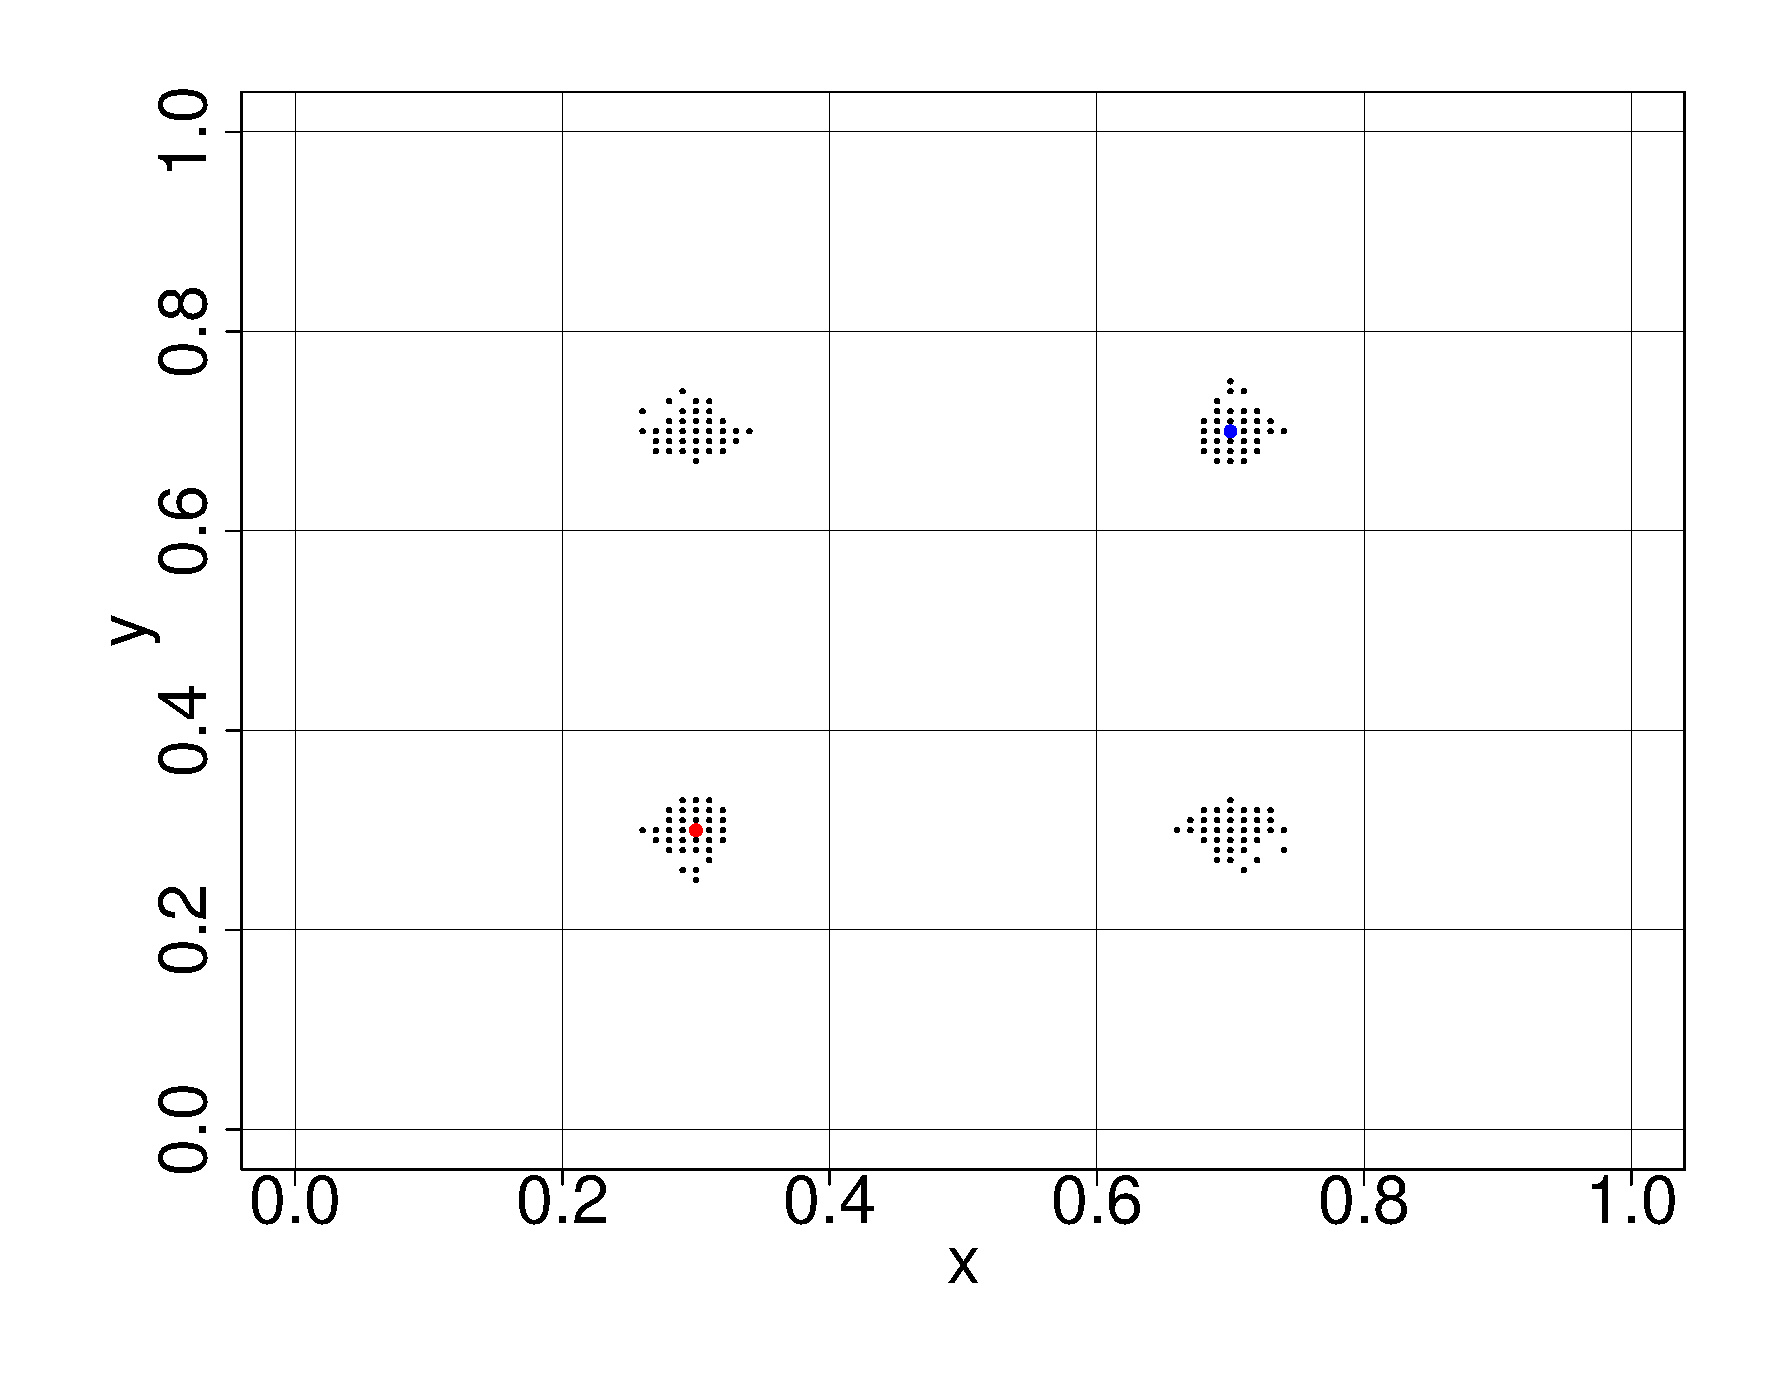
\includegraphics[height=4.5cm,width=0.35\linewidth]{../figures/sbx_a.eps}
\label{dtlz2::a}
}
\subfigure[16桁]{
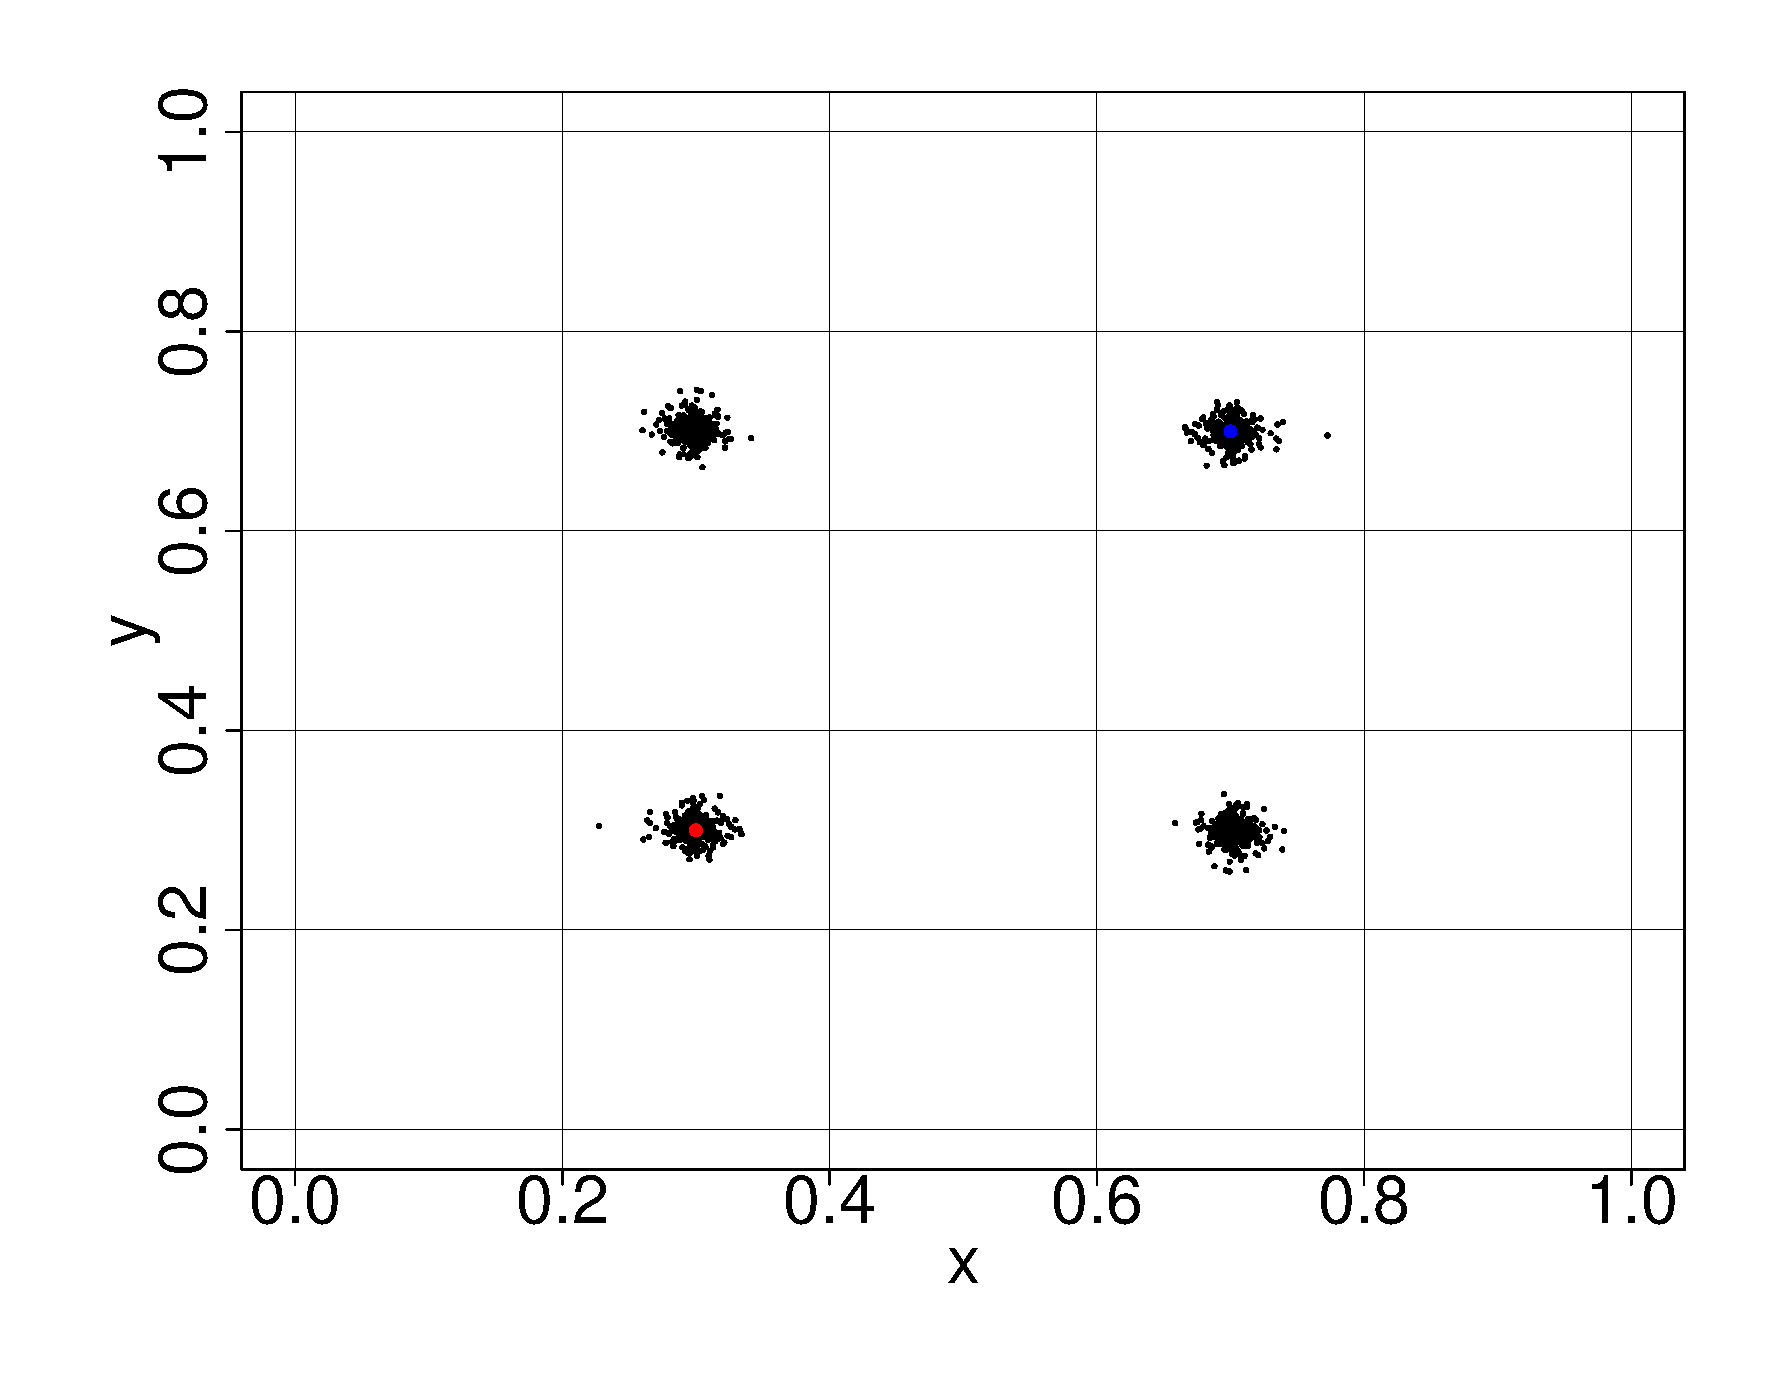
\includegraphics[height=4.5cm,width=0.35\linewidth]{../figures/sbx_b.eps}
\label{dtlz2::b}
}
\end{center}
\setlength{\abovecaptionskip}{0mm}
\setlength{\belowcaptionskip}{0mm}
\caption{制御桁数の違いによるSBXの分布比較}
\label{cross}
\end{figure}
%\vspace{-3mm}
\begin{figure}[htbp]
\begin{center}
\subfigure[2桁]{
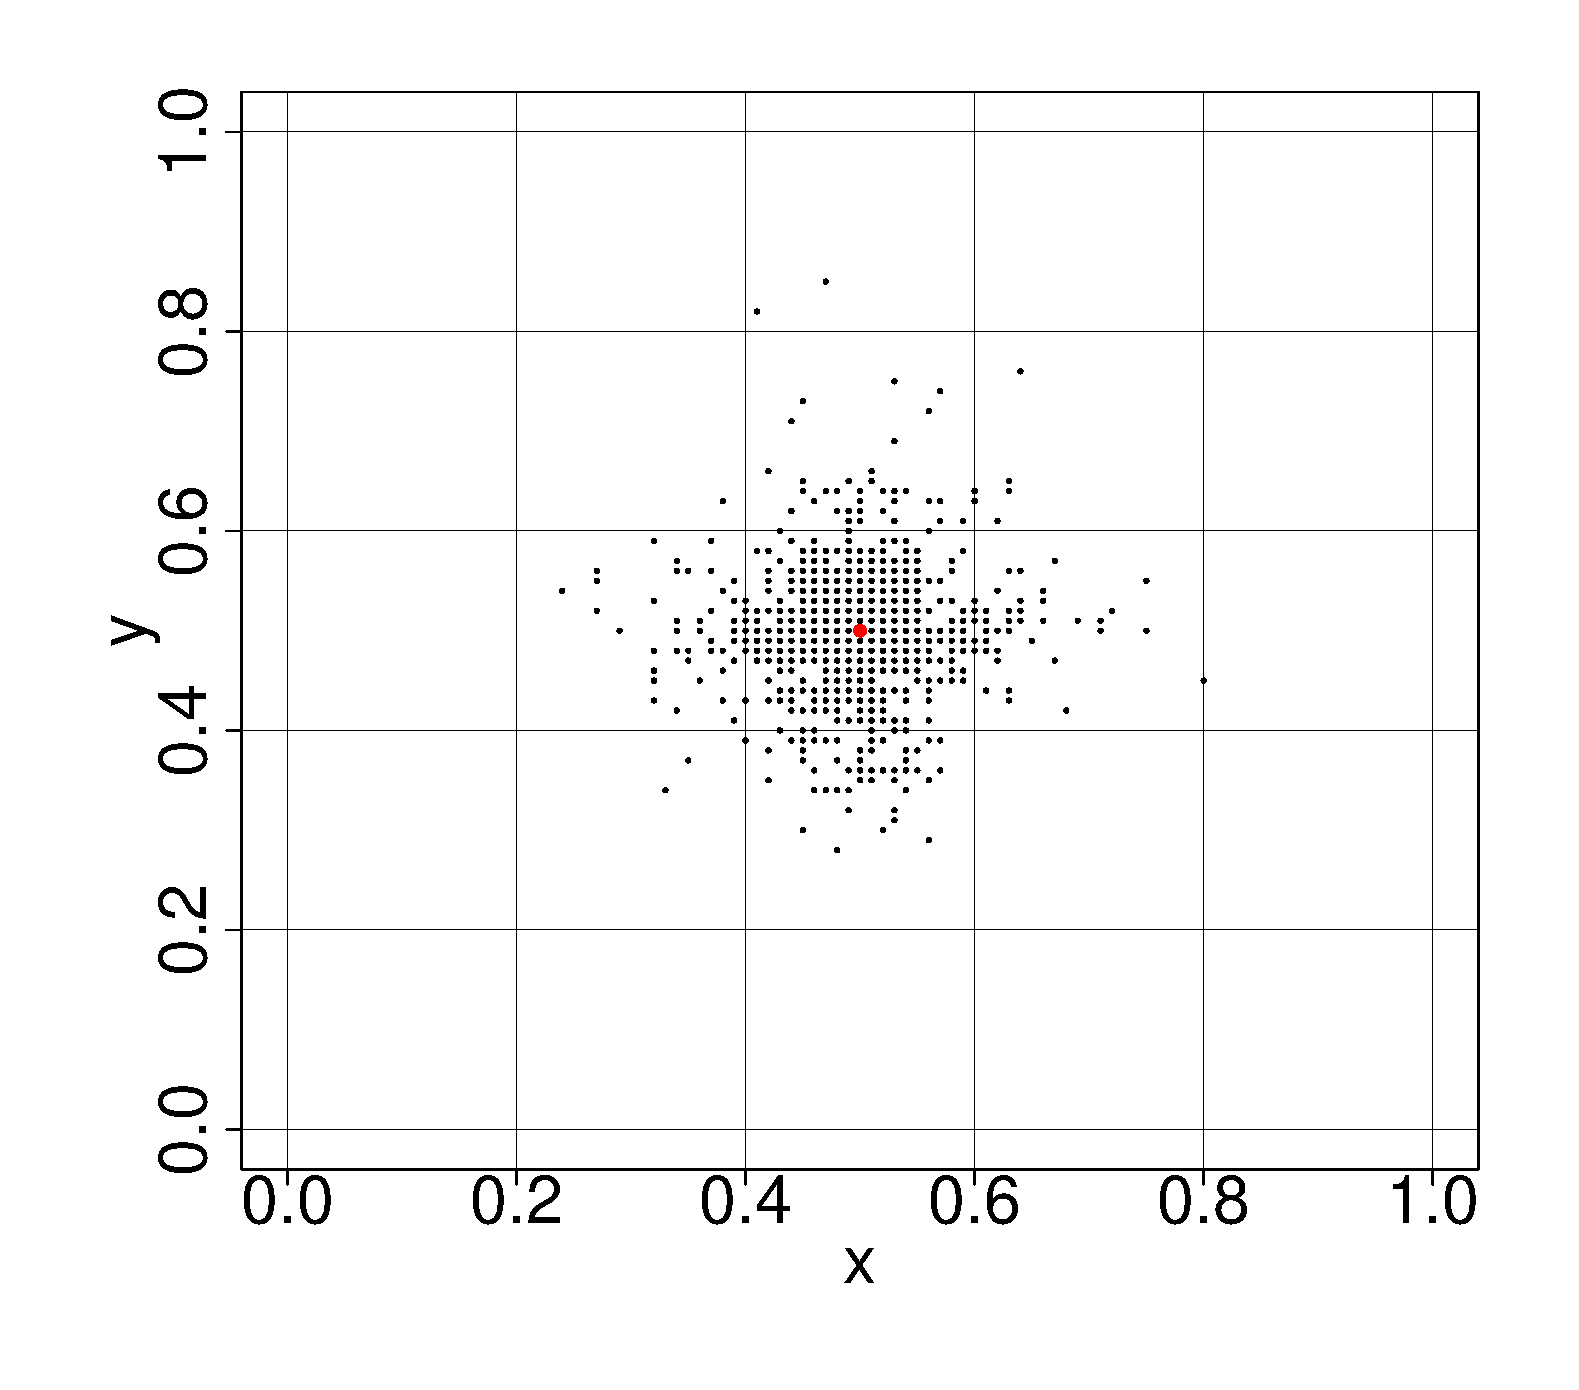
\includegraphics[width=0.35\linewidth]{../figures/mutation_a.eps}
\label{dtlz2::a}
}
\subfigure[16桁]{
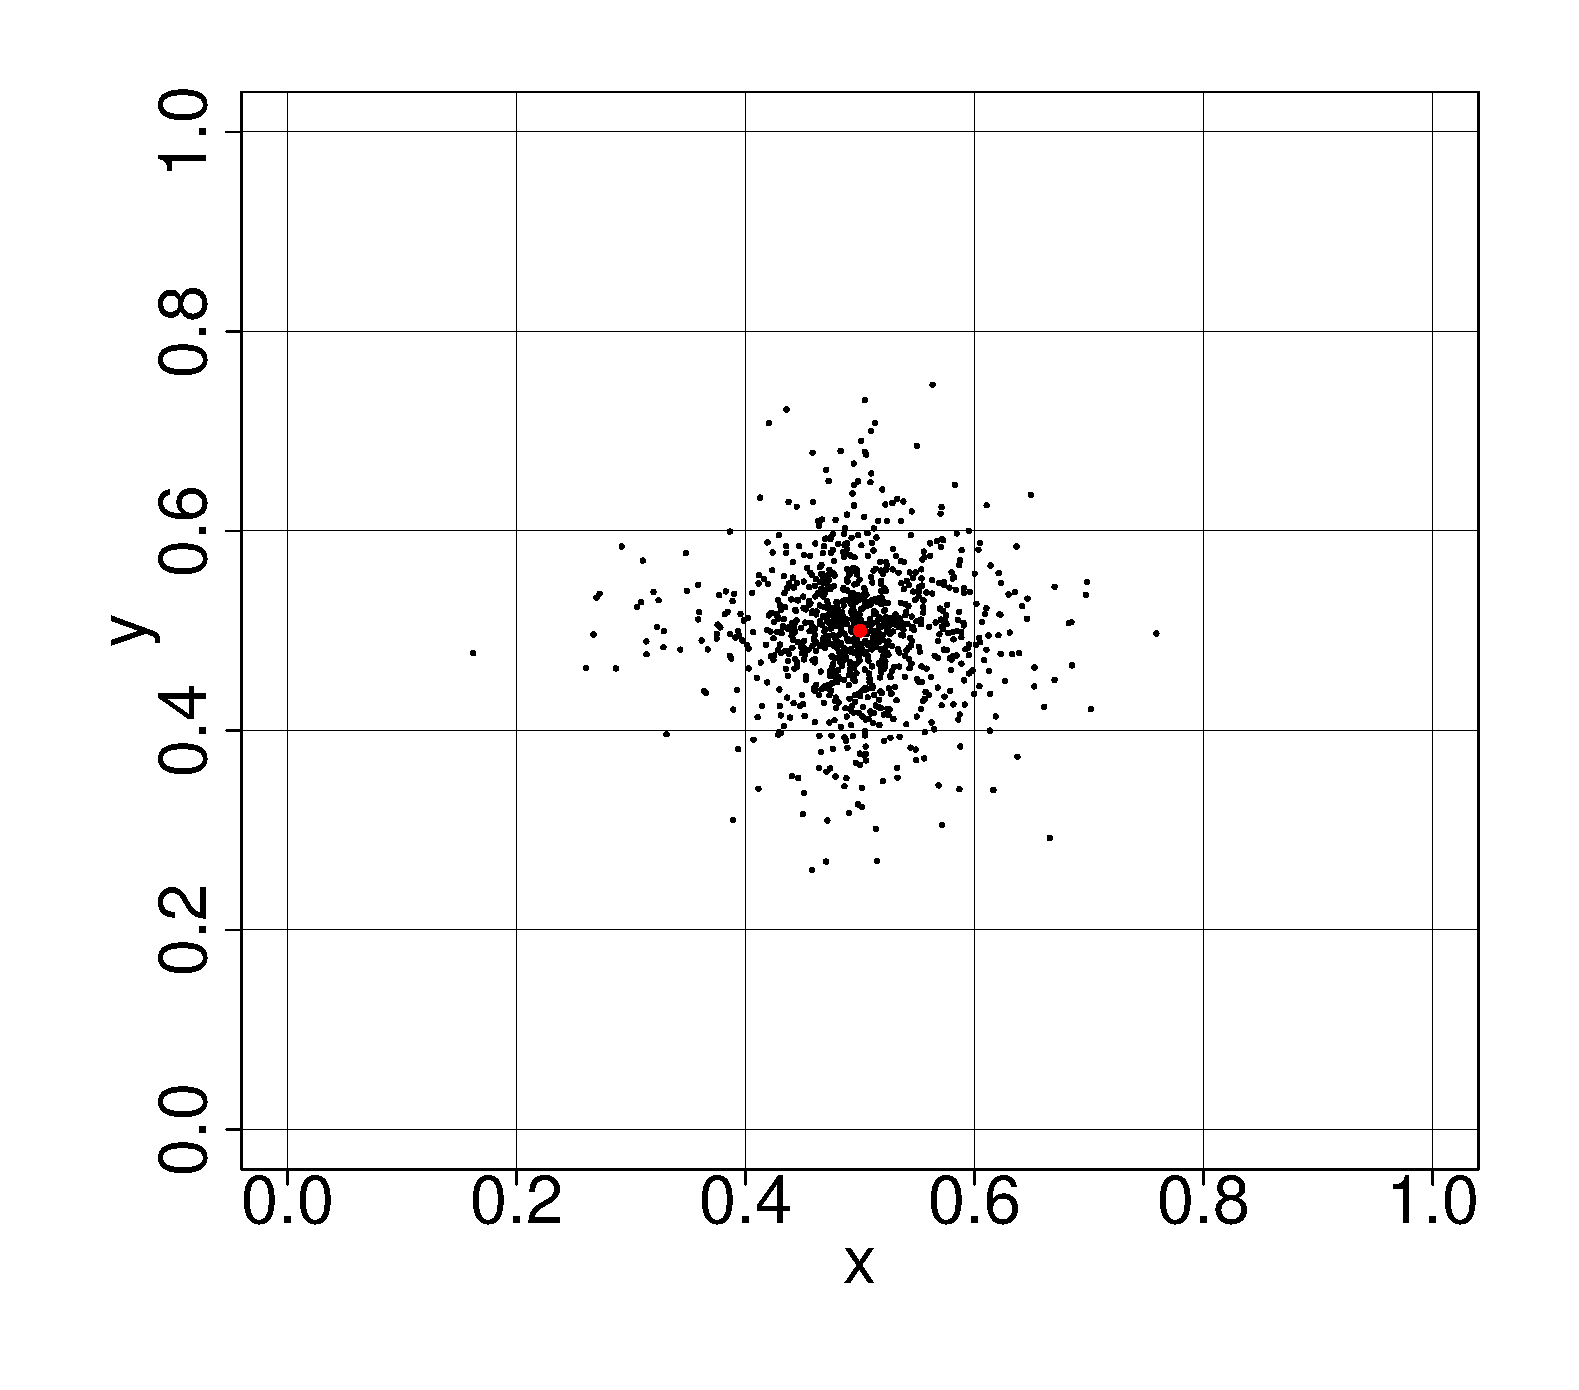
\includegraphics[width=0.35\linewidth]{../figures/mutation_b.eps}
\label{dtlz2::b}
}
\end{center}
\setlength{\abovecaptionskip}{0mm}
\setlength{\belowcaptionskip}{0mm}
\caption{制御桁数の違いによるpolynomial mutationの分布比較}
\label{mutation}
\end{figure}
%\vspace{-3mm}
\begin{figure}[H]
\begin{center}
\subfigure[SBX]{
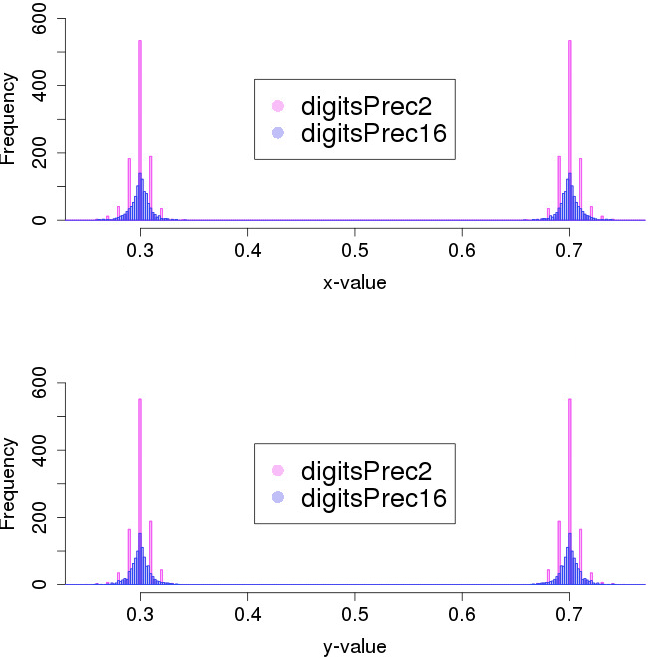
\includegraphics[width=0.45\linewidth,bb=0 0 250 250]{../figures/sbx_hist.png}
\label{hist1}
}
\subfigure[polynomial mutation]{
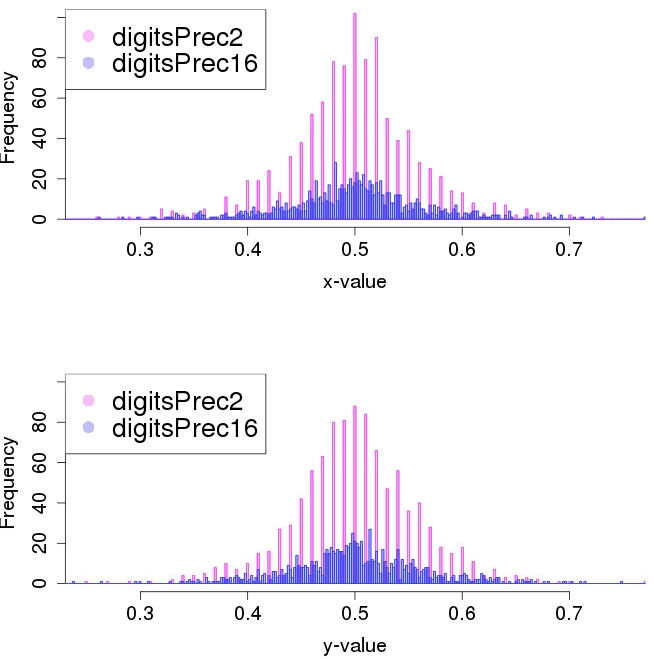
\includegraphics[width=0.45\linewidth,bb=0 0 250 250]{../figures/mutation_hist.png}
\label{hist2}
}
\end{center}
\setlength{\abovecaptionskip}{0mm}
\setlength{\belowcaptionskip}{0mm}
\caption{SBX,polynominal mutation で得られる子個体の頻度ヒストグラム}
\label{hist}
\end{figure}

\afterpage{\clearpage}

\quad この仮説を確認するため,DTLZ3の16桁において,位置変数が0もしくは1付近に生成された場合に,その位置変数の桁数を2桁にすることで,DRSsの発生が抑制され進化が効率よく行われるか試みた (Modified Method).
今回は,位置変数$x_1$,$x_2$が0.1以下もしくは0.9以上の時に桁数を2桁に落とすこととした.
計算条件は\Tabref{condition:pre}と同様である.

\quad \Figref{fig:hist}(c)は,Modified Methodを用いた場合の20世代目における位置変数$x_1$,$x_2$の累積頻度ヒストグラムを示したものである.
%また,\Tabref{tbl:mod}はDTLZ3において小数点以下$2$桁,$16$桁で制御し最適化を行った場合とModified Methodを使用した場合のGDとIGDの平均値の推移を示している.
また,\Figref{fig:mod}(a),(b)には各桁数とModified Methodを用いた場合のGD,IGDの推移を,(c)にはModified Methodを使用した場合に最終的に得られた非劣解の分布を示す.

\quad \Figref{fig:hist}より,Modified Methodは16桁と比較し,明らかに0もしくは1付近の解の分布の頻度が減少していることが分かる.
このことから,DTLZ3においては,桁数を小さくする(粗く離散化する)ことがDRSsの発生を抑制することに繋がっていることが分かった.
また,\Figref{fig:mod}(a),(b)より,Modified Methodは2桁には及ばないものの,16桁と比較しGD・IGDいずれも小さい値となっていることが分かる.
このことからも,桁数を小さくすることでDRSsの発生が抑制されたため,効率的に進化が進み収束性や多様性が向上したものと考えられる.
さらに,\Figref{fig:mod}(c)より,ややDRSsは残っているものの,16桁(\Figref{non_b}(b))と比較すると減少していることが分かる.

\quad 以上より,先行研究においては,NSGA-IIと16個の多目的ベンチマーク問題を用いて設計変数の離散化の影響を評価した結果,粗く離散化するほど解の収束速度が向上することが分かった.
一方で,DTLZ4等の非線形性が非常に強い問題では,粗く離散化しすぎると解の多様性が失われてしまう可能性があることが分かった.
また,DTLZ3においては,粗く離散化することでDRSsの発生が避けられ,解の収束性が向上したことが確認できた.
これらの結果から,問題に応じて各設計変数を適切に設定することで,効率的に探索を進めることができる可能性があることが分かった.
さらに,動的に離散化する大きさを変更することが,効率的探索に繋がる可能性を示唆した.

\quad しかしながら,先行研究ではNSGA-IIのみでしか影響が評価されておらず,ベンチマーク問題もDTLZ問題のみであったため,他の実数値GAやベンチマーク問題においても同様の現象が確認できるかなど,未だ不明確な部分も多い.
また,設計変数の離散化の活用法についても,研究の余地が残されている.
%したがって,先行研究の結果の一般性の確認と共に,設計変数の離散化の有効な活用方法を検討することが必要であると考えられる.

\quad そこで本研究では,先行研究のNSGA-IIに加え,代表的実数値GAの一つであるMOEA/Dでの検証を行い,様々な特徴を持つ19個のベンチマーク問題を用いて影響を評価する.
また,設計変数の離散化の活用法を考察し,効率的探索に繋がる手法の提案を行う.
%先行研究における今後の課題として,最適化を行う前に適切に離散化を行うことが難しいことが挙げられていた.
%
%そこで,本研究では,設計変数を適応的に離散化を行うことで,効率的探索を行う手法を提案することを目的とし研究を進める.
%
%
\begin{figure*}[htbp]
\begin{tabular}{ccc}
\begin{minipage}{0.333\hsize}
\centering
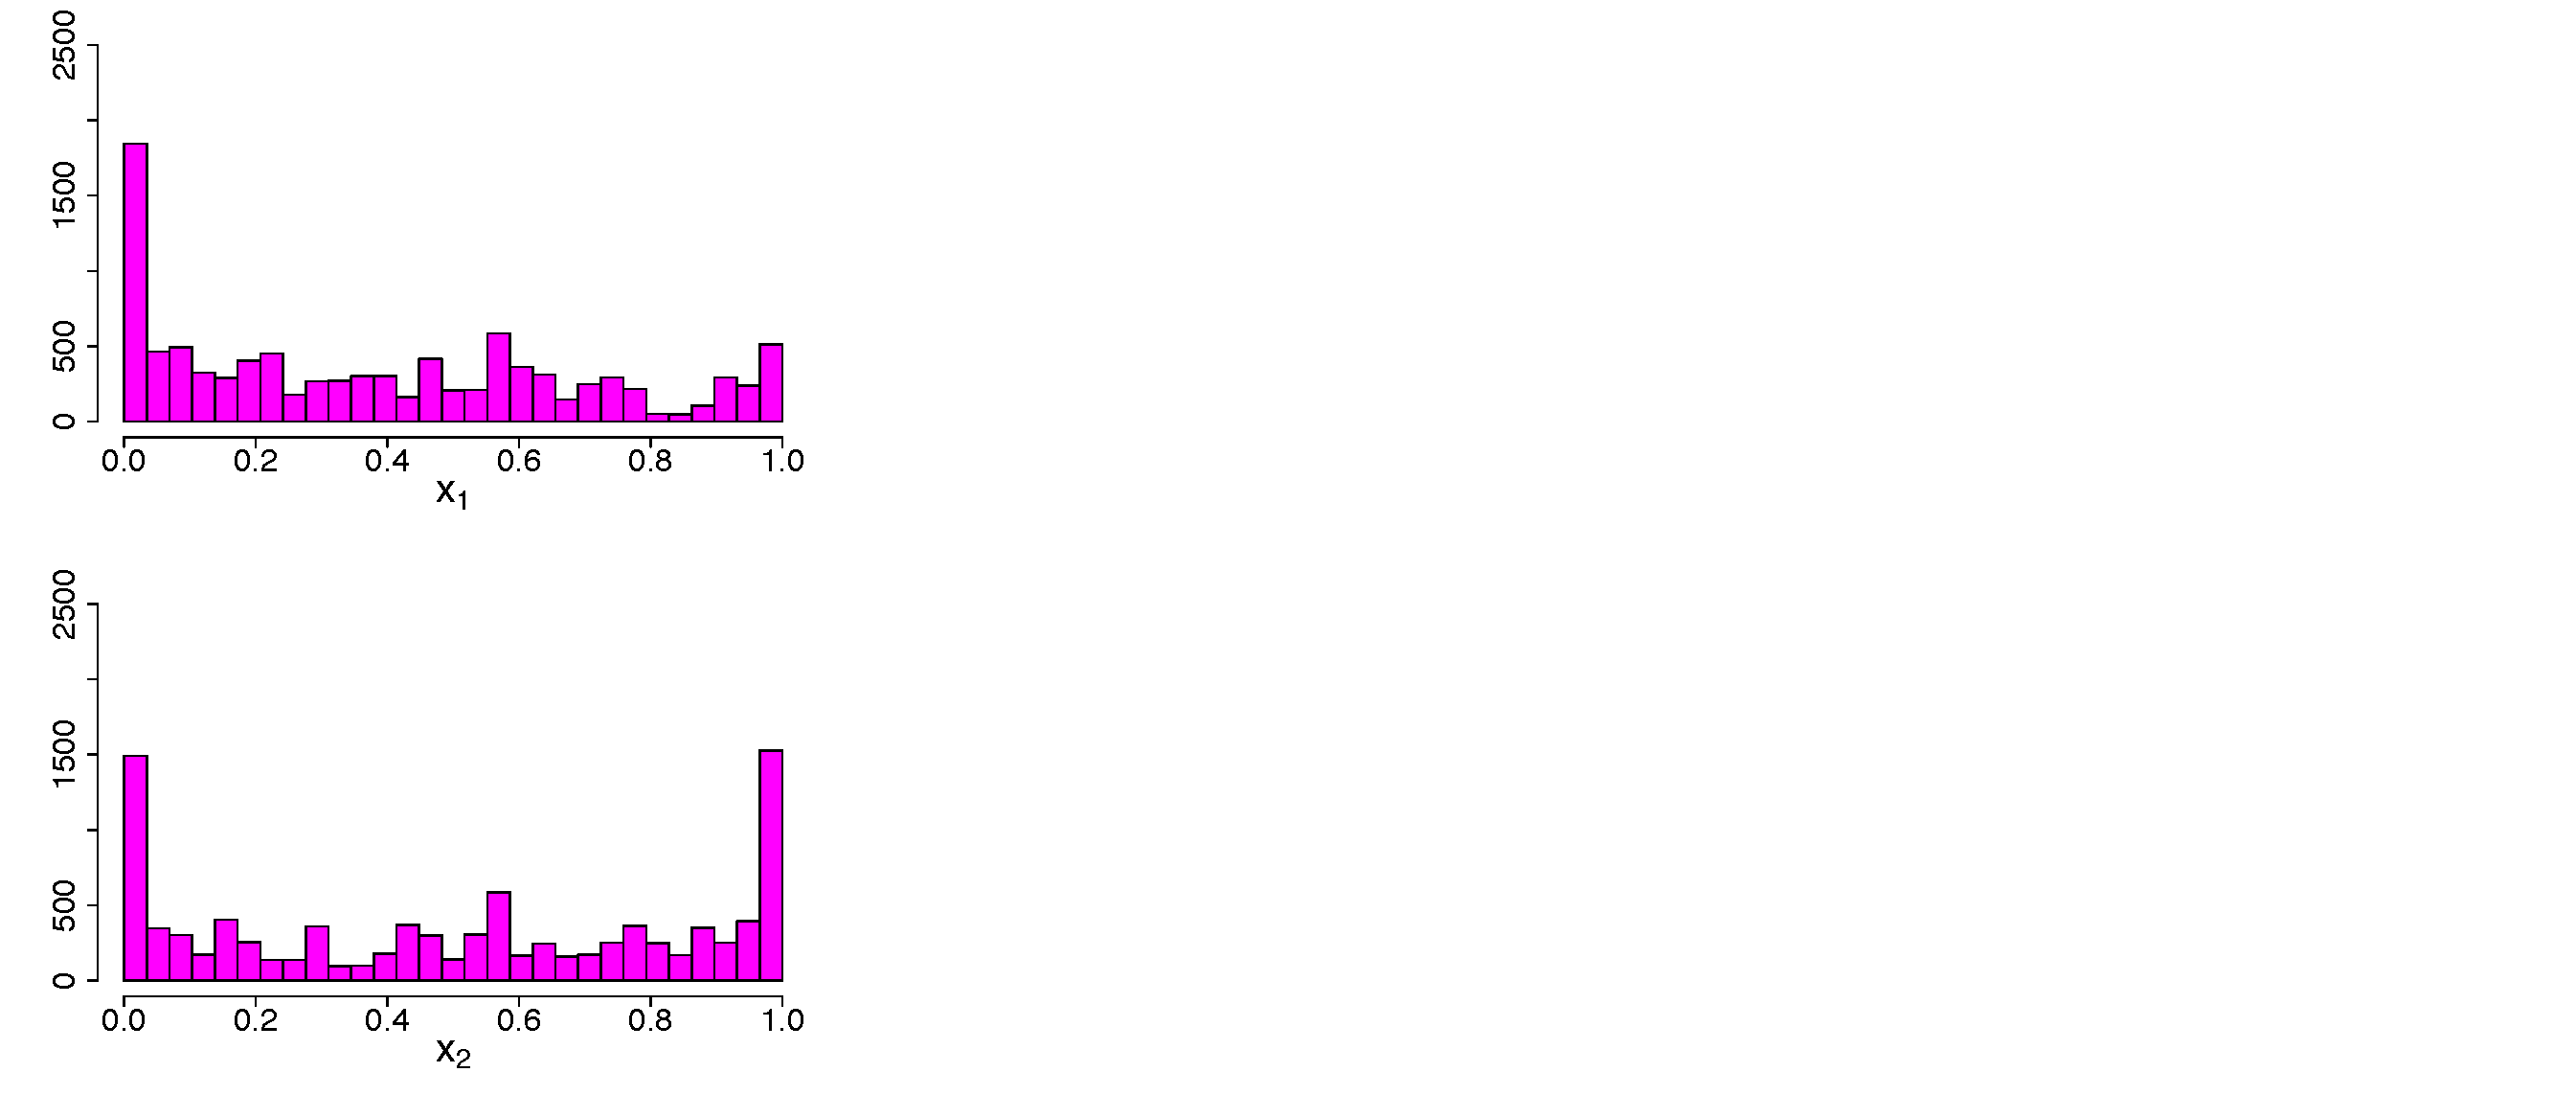
\includegraphics[height=4.5cm,width=0.8\linewidth]{../figures/kaizen_hist_digi2.pdf}
%\setlength{\abovecaptionskip}{-8mm}
%\setlength{\belowcaptionskip}{-5mm}
%\caption{a}
\begin{center}
{\footnotesize (a) 2-digit}
\end{center}
\end{minipage}
%\hspace{-1mm}
\begin{minipage}{0.333\hsize}
\centering
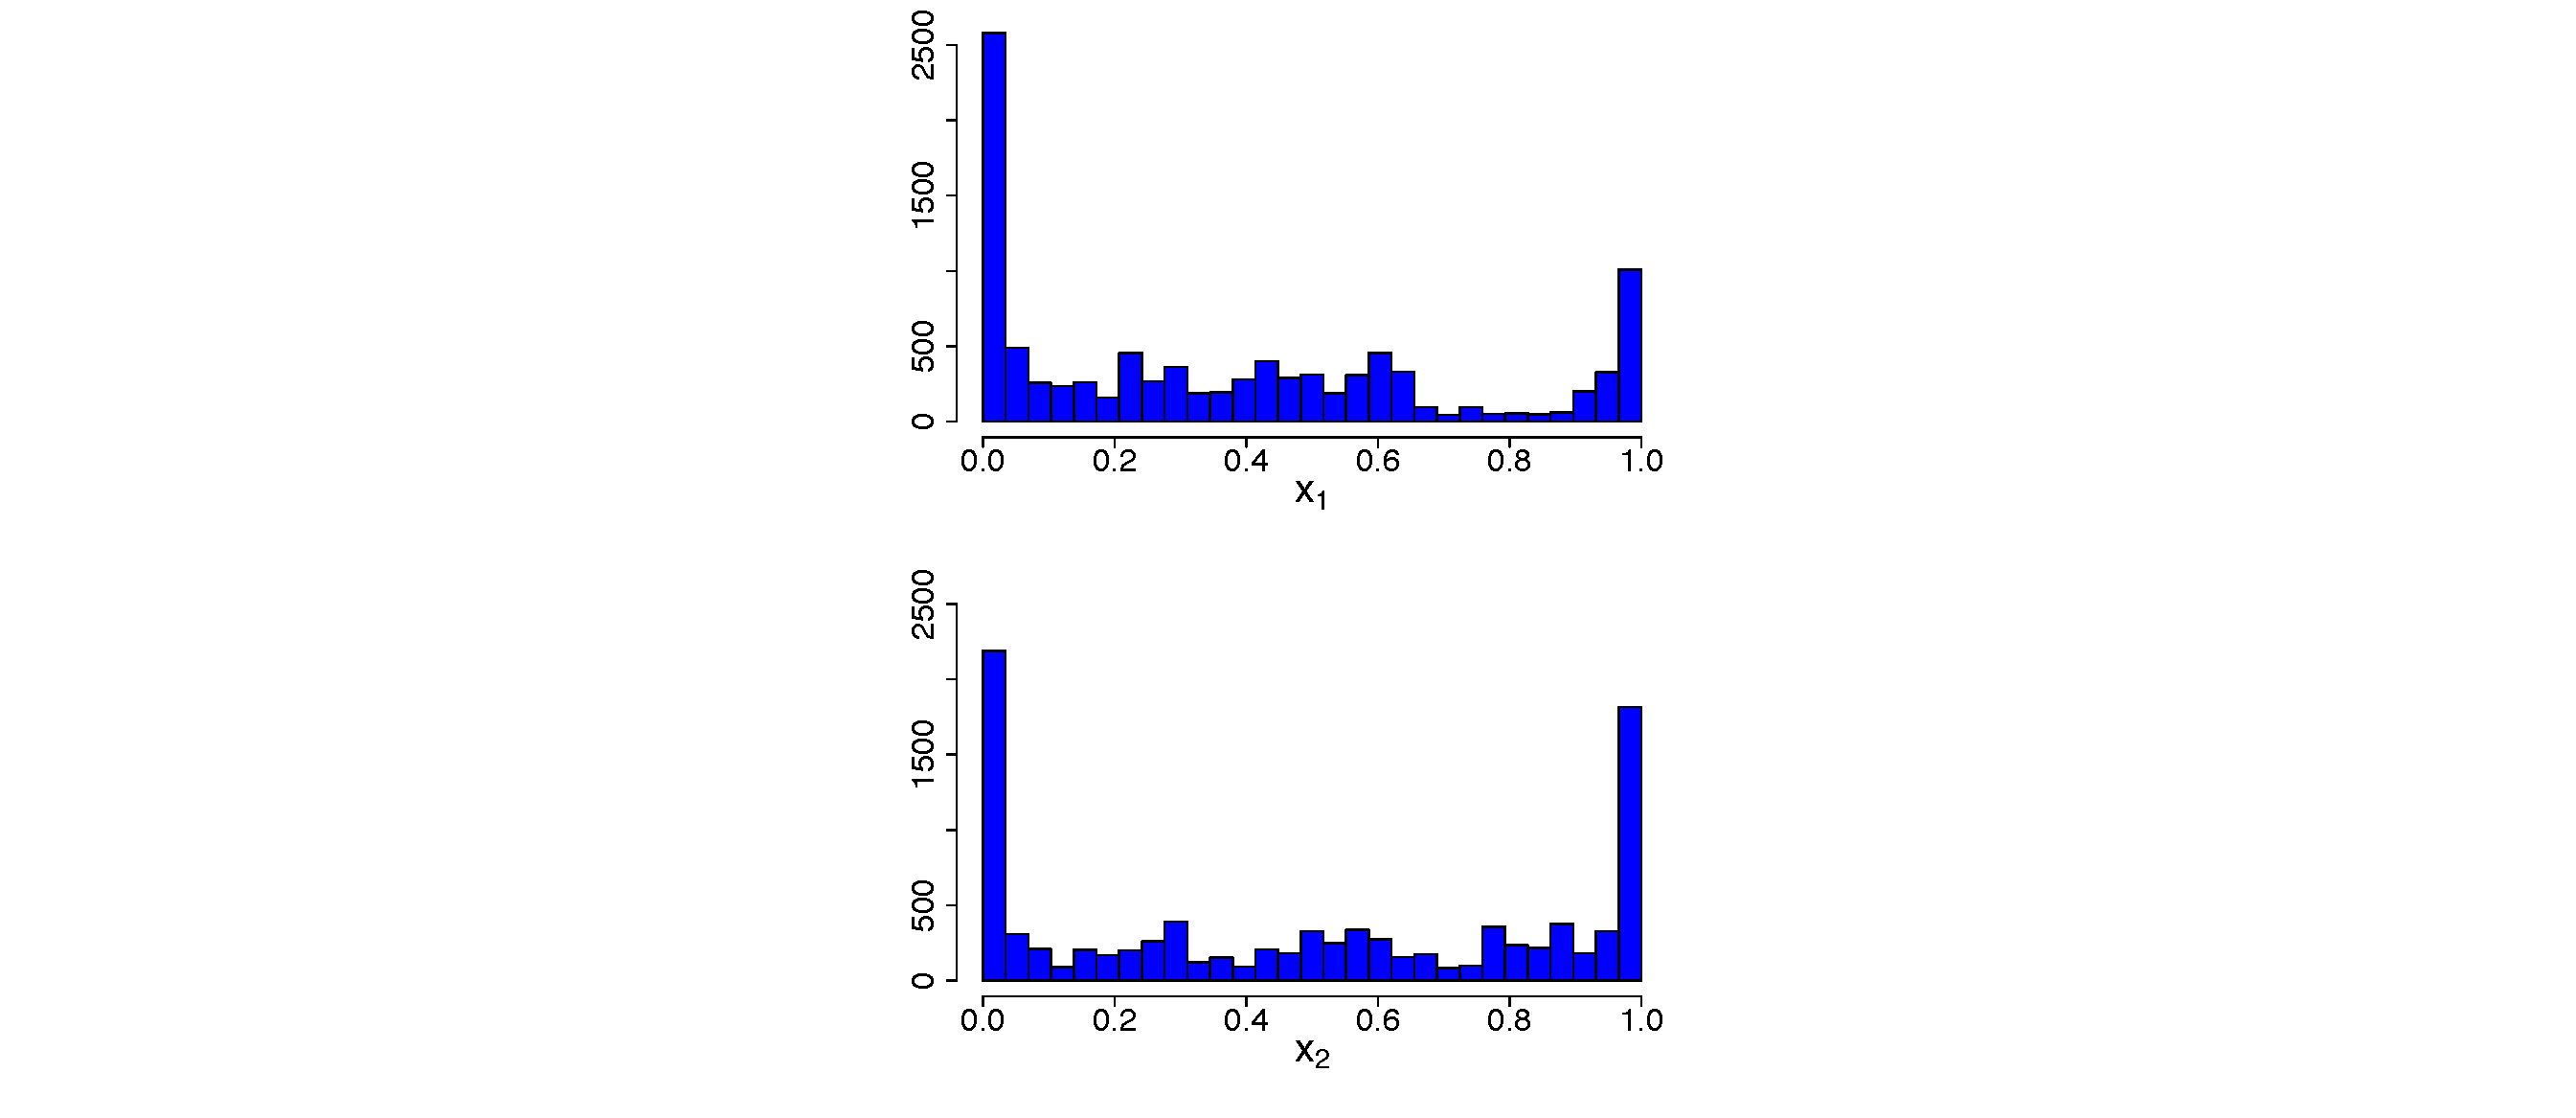
\includegraphics[height=4.5cm,width=0.8\linewidth]{../figures/kaizen_hist_digi16.pdf}
%\setlength{\abovecaptionskip}{-8mm}
%\setlength{\belowcaptionskip}{-5mm}
%\caption{a}
\begin{center}
{\footnotesize (b) 16-digit}
\end{center}
\end{minipage}
\begin{minipage}{0.333\hsize}
\centering
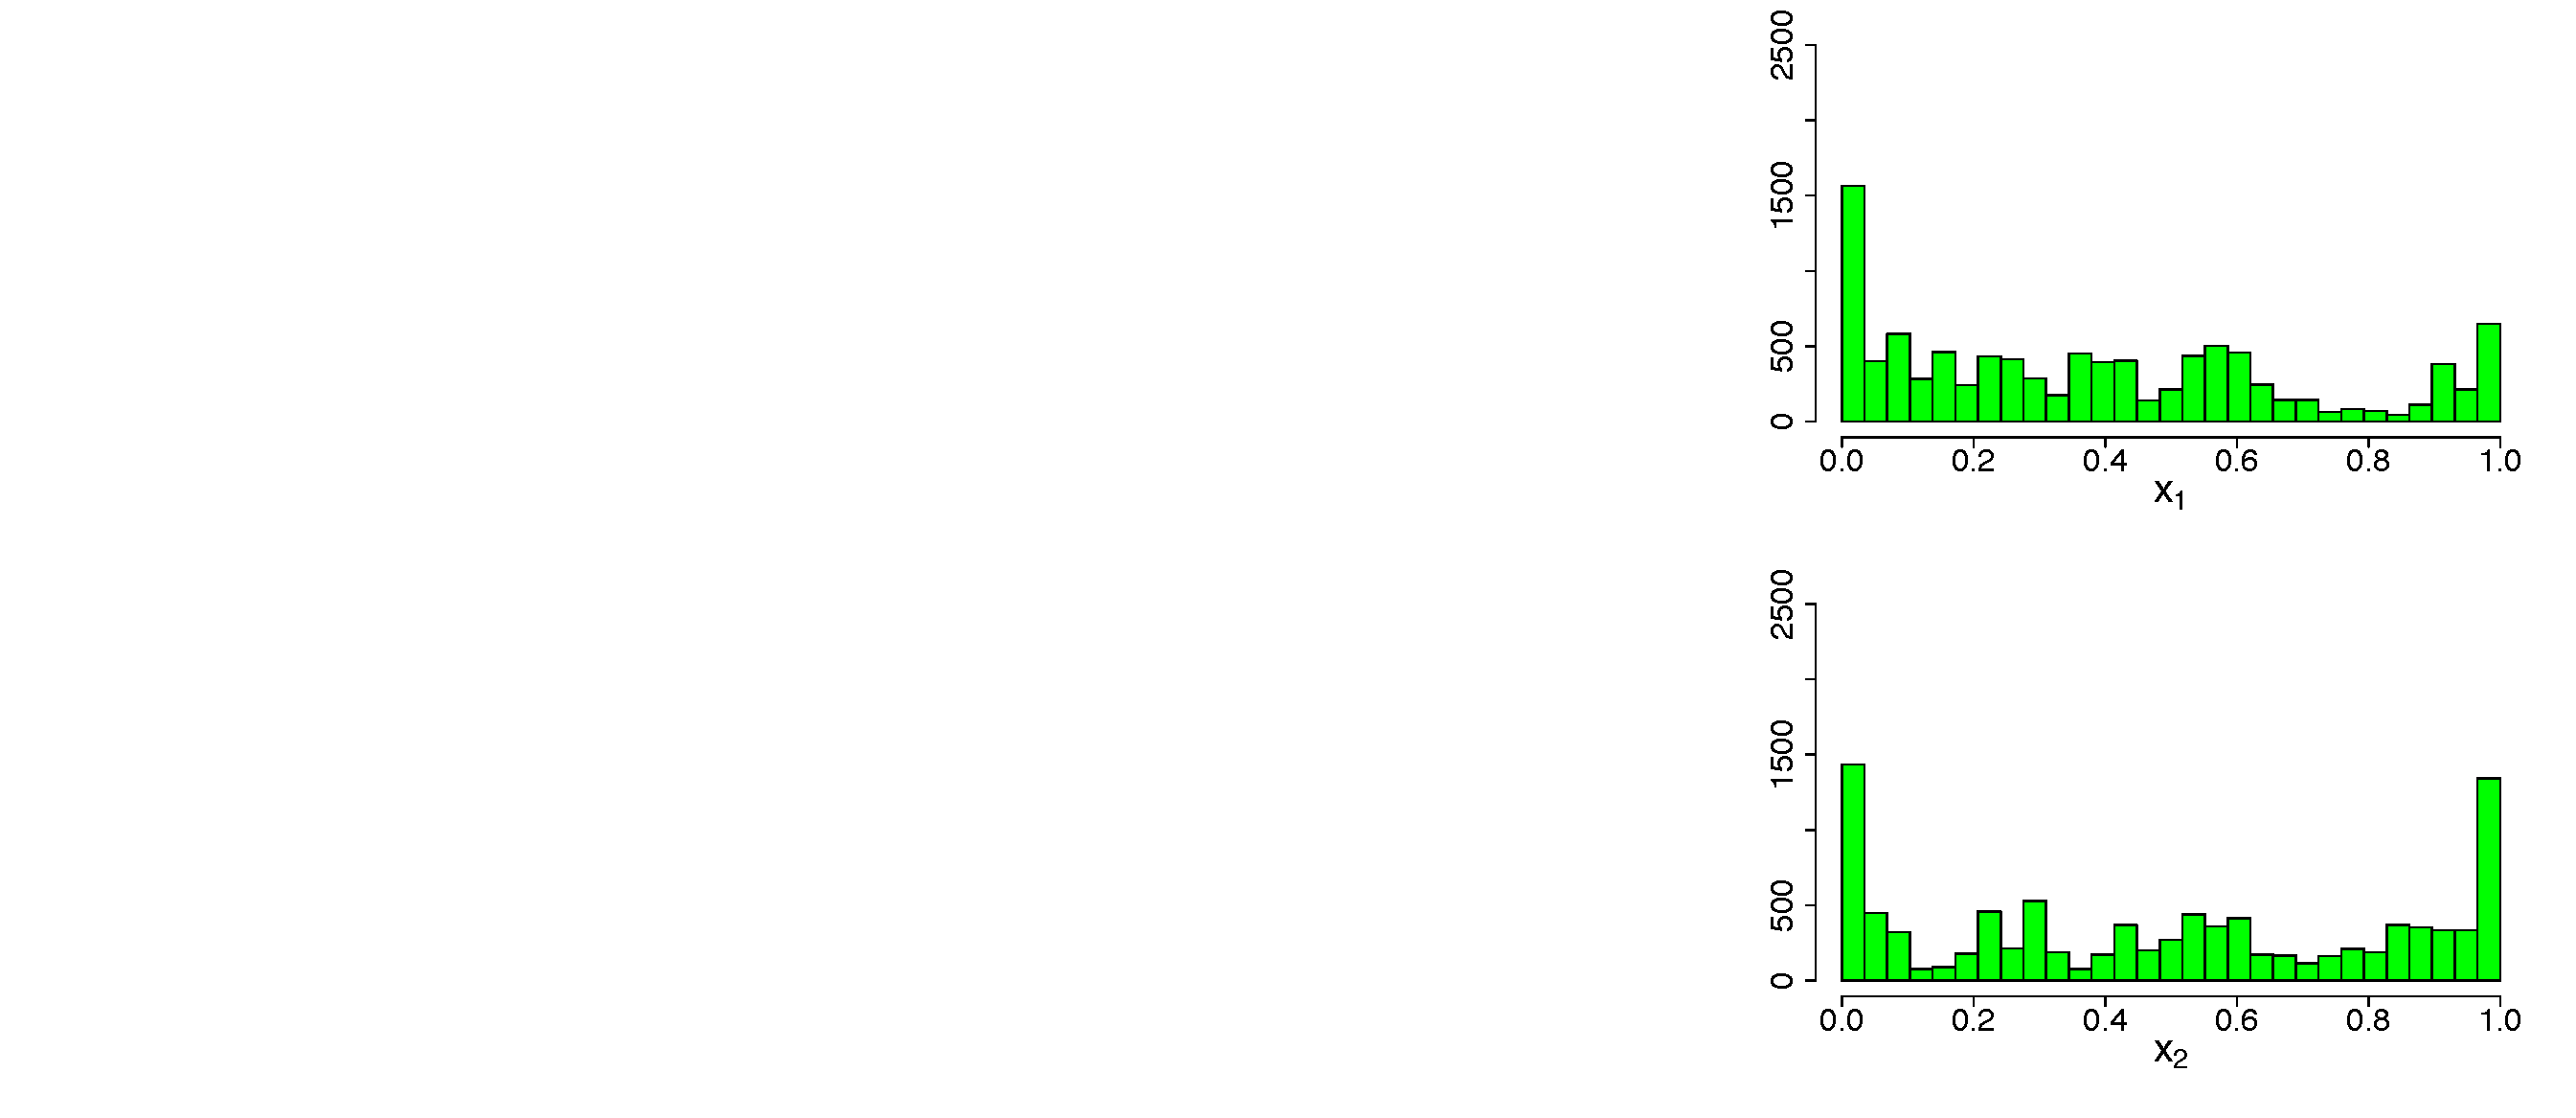
\includegraphics[height=4.5cm,width=0.8\linewidth]{../figures/kaizen_hist_mod.pdf}
%\setlength{\abovecaptionskip}{-8mm}
%\setlength{\belowcaptionskip}{-5mm}
%\caption{a}
\begin{center}
{\footnotesize (c) modified 16-digit}
\end{center}
\end{minipage}
\end{tabular}
\caption{2桁,16桁,Modified Methodにおける位置変数$x_1$,$x_2$の累積頻度ヒストグラム}%Cumulative-frequency histograms of position variables x1 and x2 obtained using 2- and 16- and modified 16-digit.
\label{fig:hist}
%\setlength\textfloatsep{-5mm}
\end{figure*}
%
%\begin{table*}[htbp]
%\centering
%\caption{Averaged GD and IGD at 10th, half and final generation for using 2-digit, 16-digit, modified 16-digit on DTLZ3.
%Best performance is shown in bold.}
%\fontsize{8pt}{8pt} \selectfont
%\tabcolsep = 3pt
%\label{tbl:mod}
%\begin{tabular}{c|ccccc|c|c|c}
%\hline 
%problem & MG & PS & Obj. & Var. & Gen & 2-digit & 16-digit & Modified Method (16-digit)\\ 
%%\cmidrule(r){3-9}
%%\hline 
%\cline{7-9}
%&&&&&&GD&GD&GD\\
%%\cline{3-5}
%\hline
%\multirow{3}{*}{DTLZ3}&     &&   &       & 10 &$\bf{2.191 \times 10^{3}}$ & $2.508 \times 10^{3}$ & $2.210 \times 10^{3}$ \\
%  				   & 200 & 500 & 3 & 38 & 100 &$\bf{9.935 \times 10}$   & $4.039 \times 10^{2}$ & $1.554 \times 10^{2}$ \\
%				   &        &       && &200 &\bf{6.521} & $6.669 \times 10$ & $2.345 \times 10$ \\
%
%\hline
%\hline
%%\cline{5-9}
%&&&&&&IGD&IGD&IGD\\
%%\cline{3-5}
%\hline
%\multirow{3}{*}{DTLZ3} &        &   &&    & 10 &$\bf{1.657 \times 10^{3}}$ & $1.666 \times 10^{3}$ & $1.675 \times 10^{3}$ \\
%  				   &200 & 500 & 3 & 38 & 100 &$\bf{6.871 \times 10}$ &  $2.195 \times 10^{2}$ & $1.090 \times 10^{2}$ \\
%				   &        &      &&  &200 & \bf{5.059} & $4.607 \times 10$ & $1.867 \times 10$ \\				   
%\hline\end{tabular}
%\end{table*}
%
%
\begin{figure*}[htbp]
\begin{tabular}{cc}
\begin{minipage}{0.32\hsize}
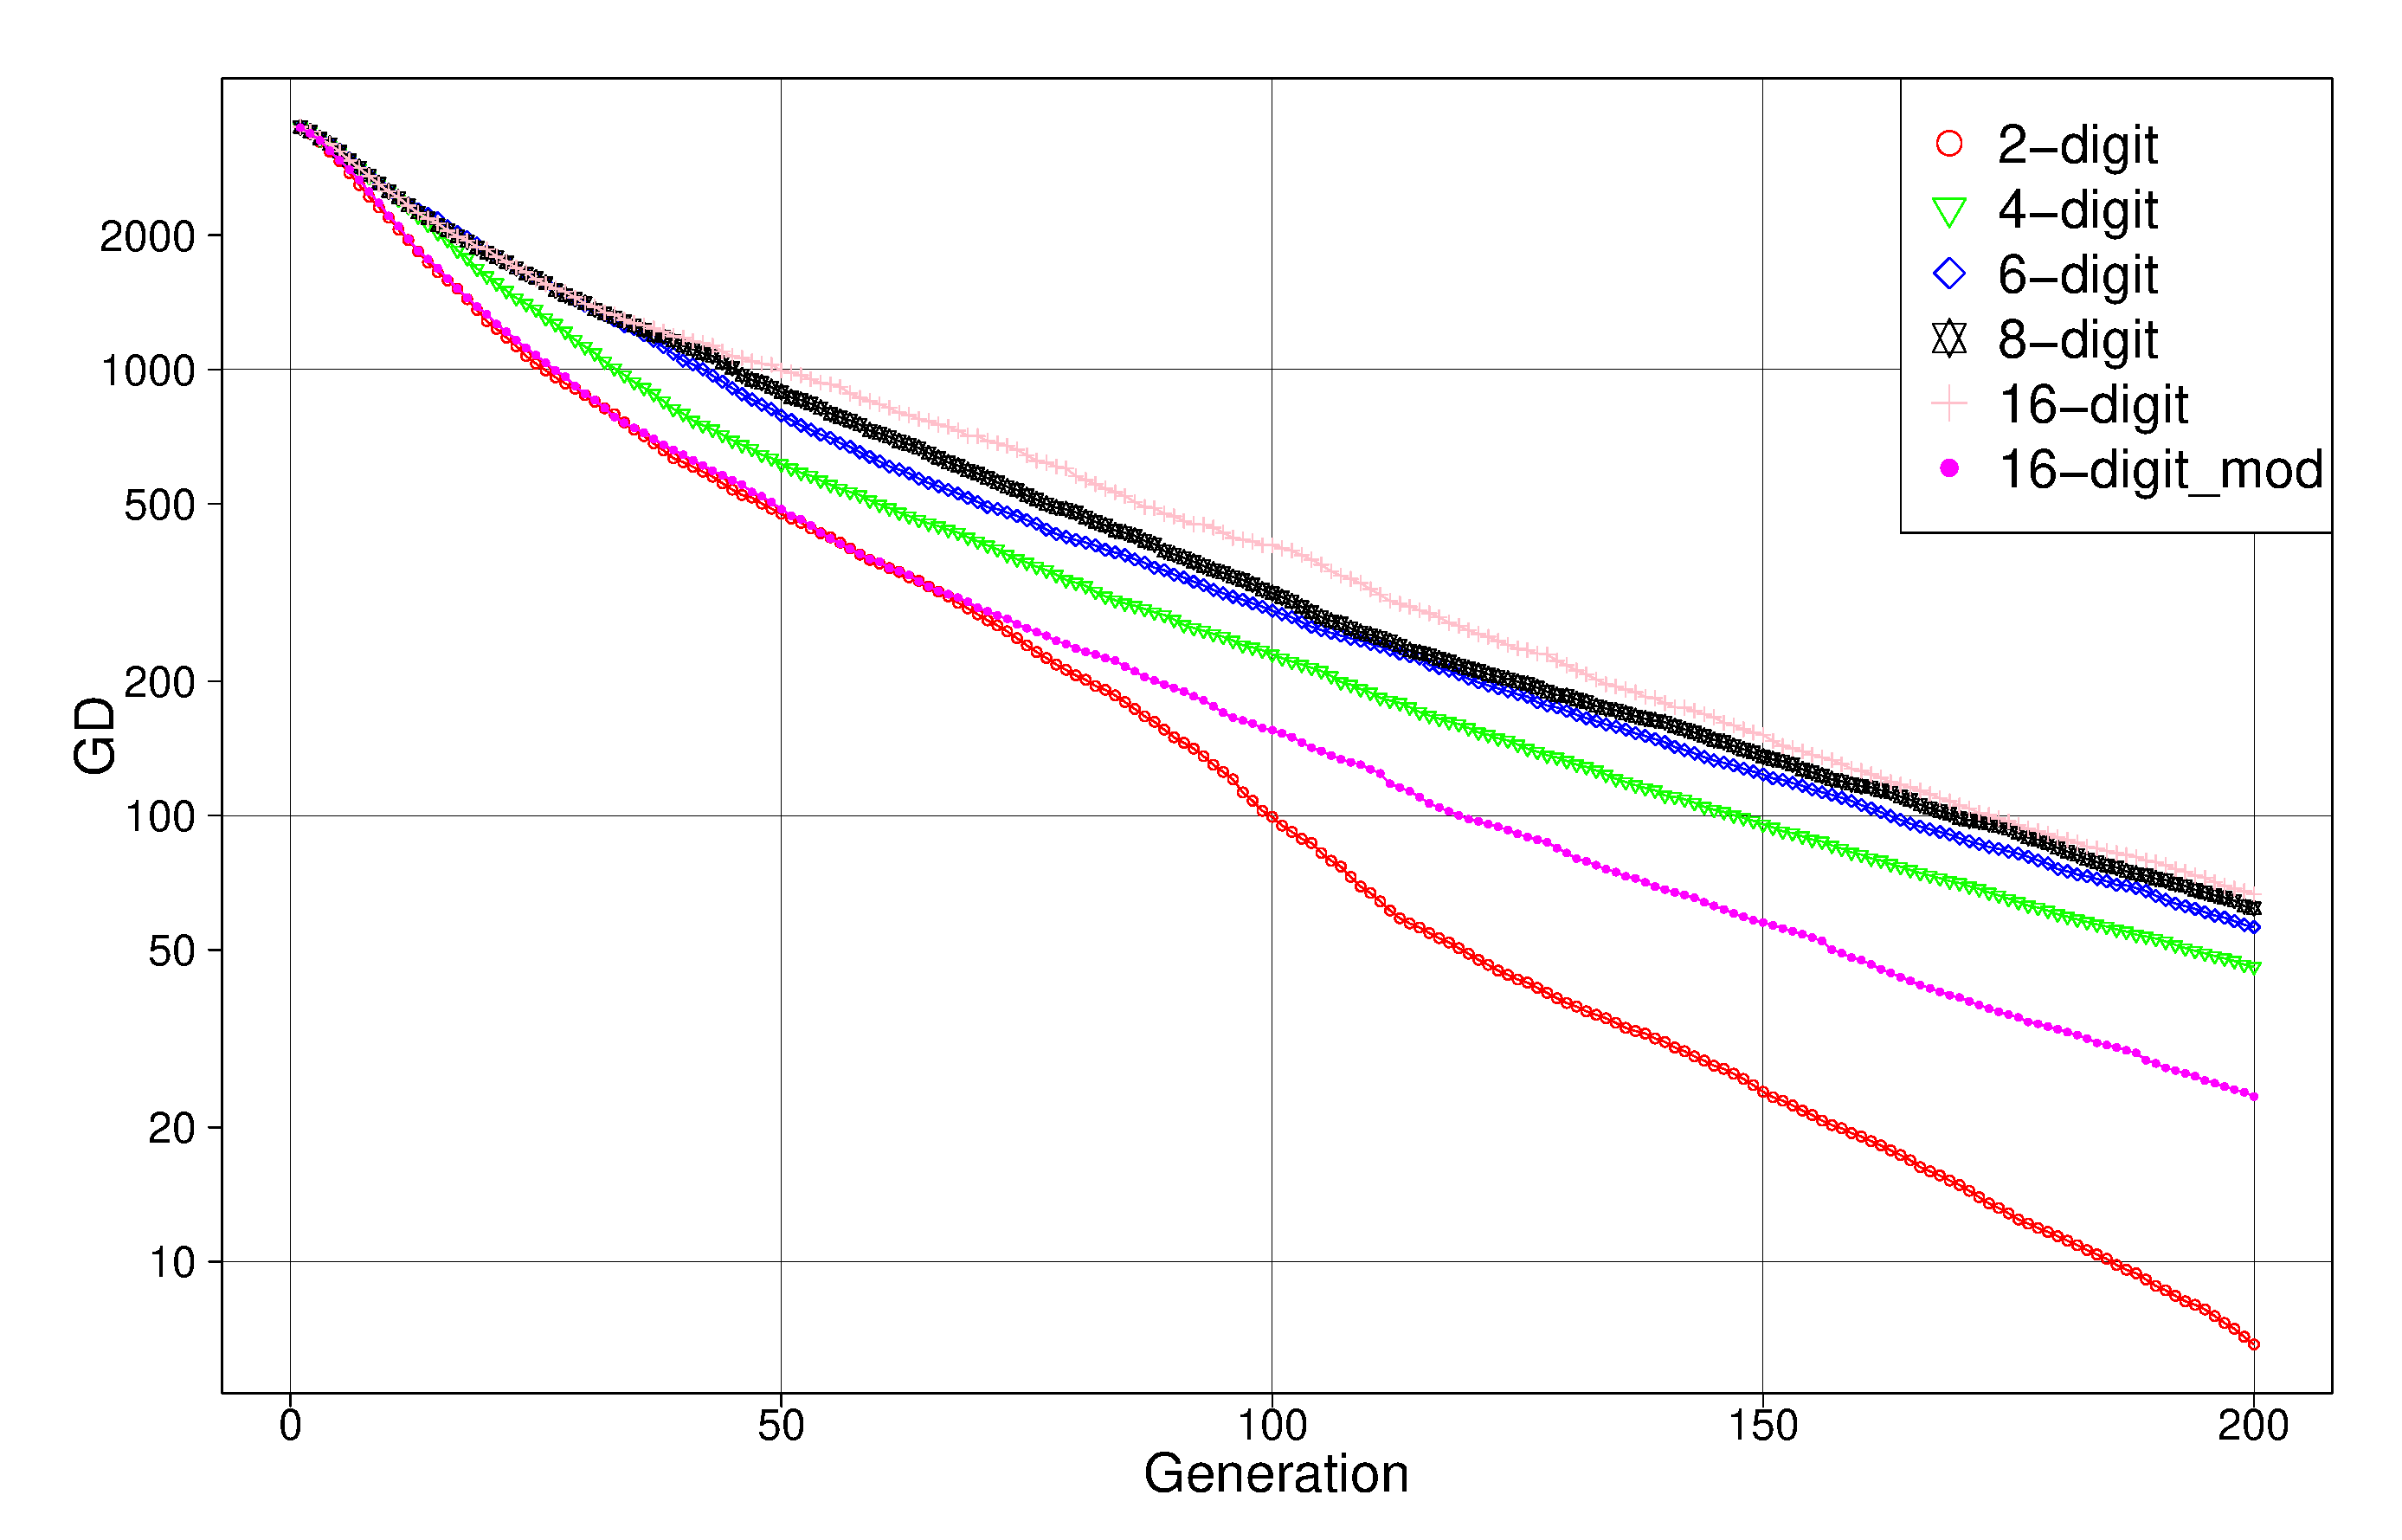
\includegraphics[width=1\linewidth]{../figures/DTLZ3_modified_GD.eps}
%\setlength{\abovecaptionskip}{-8mm}
%\setlength{\belowcaptionskip}{-5mm}
%\caption{a}
\begin{center}
{\footnotesize (a) History of GD}
\end{center}
\end{minipage}
%\hspace{-1mm}
\begin{minipage}{0.32\hsize}
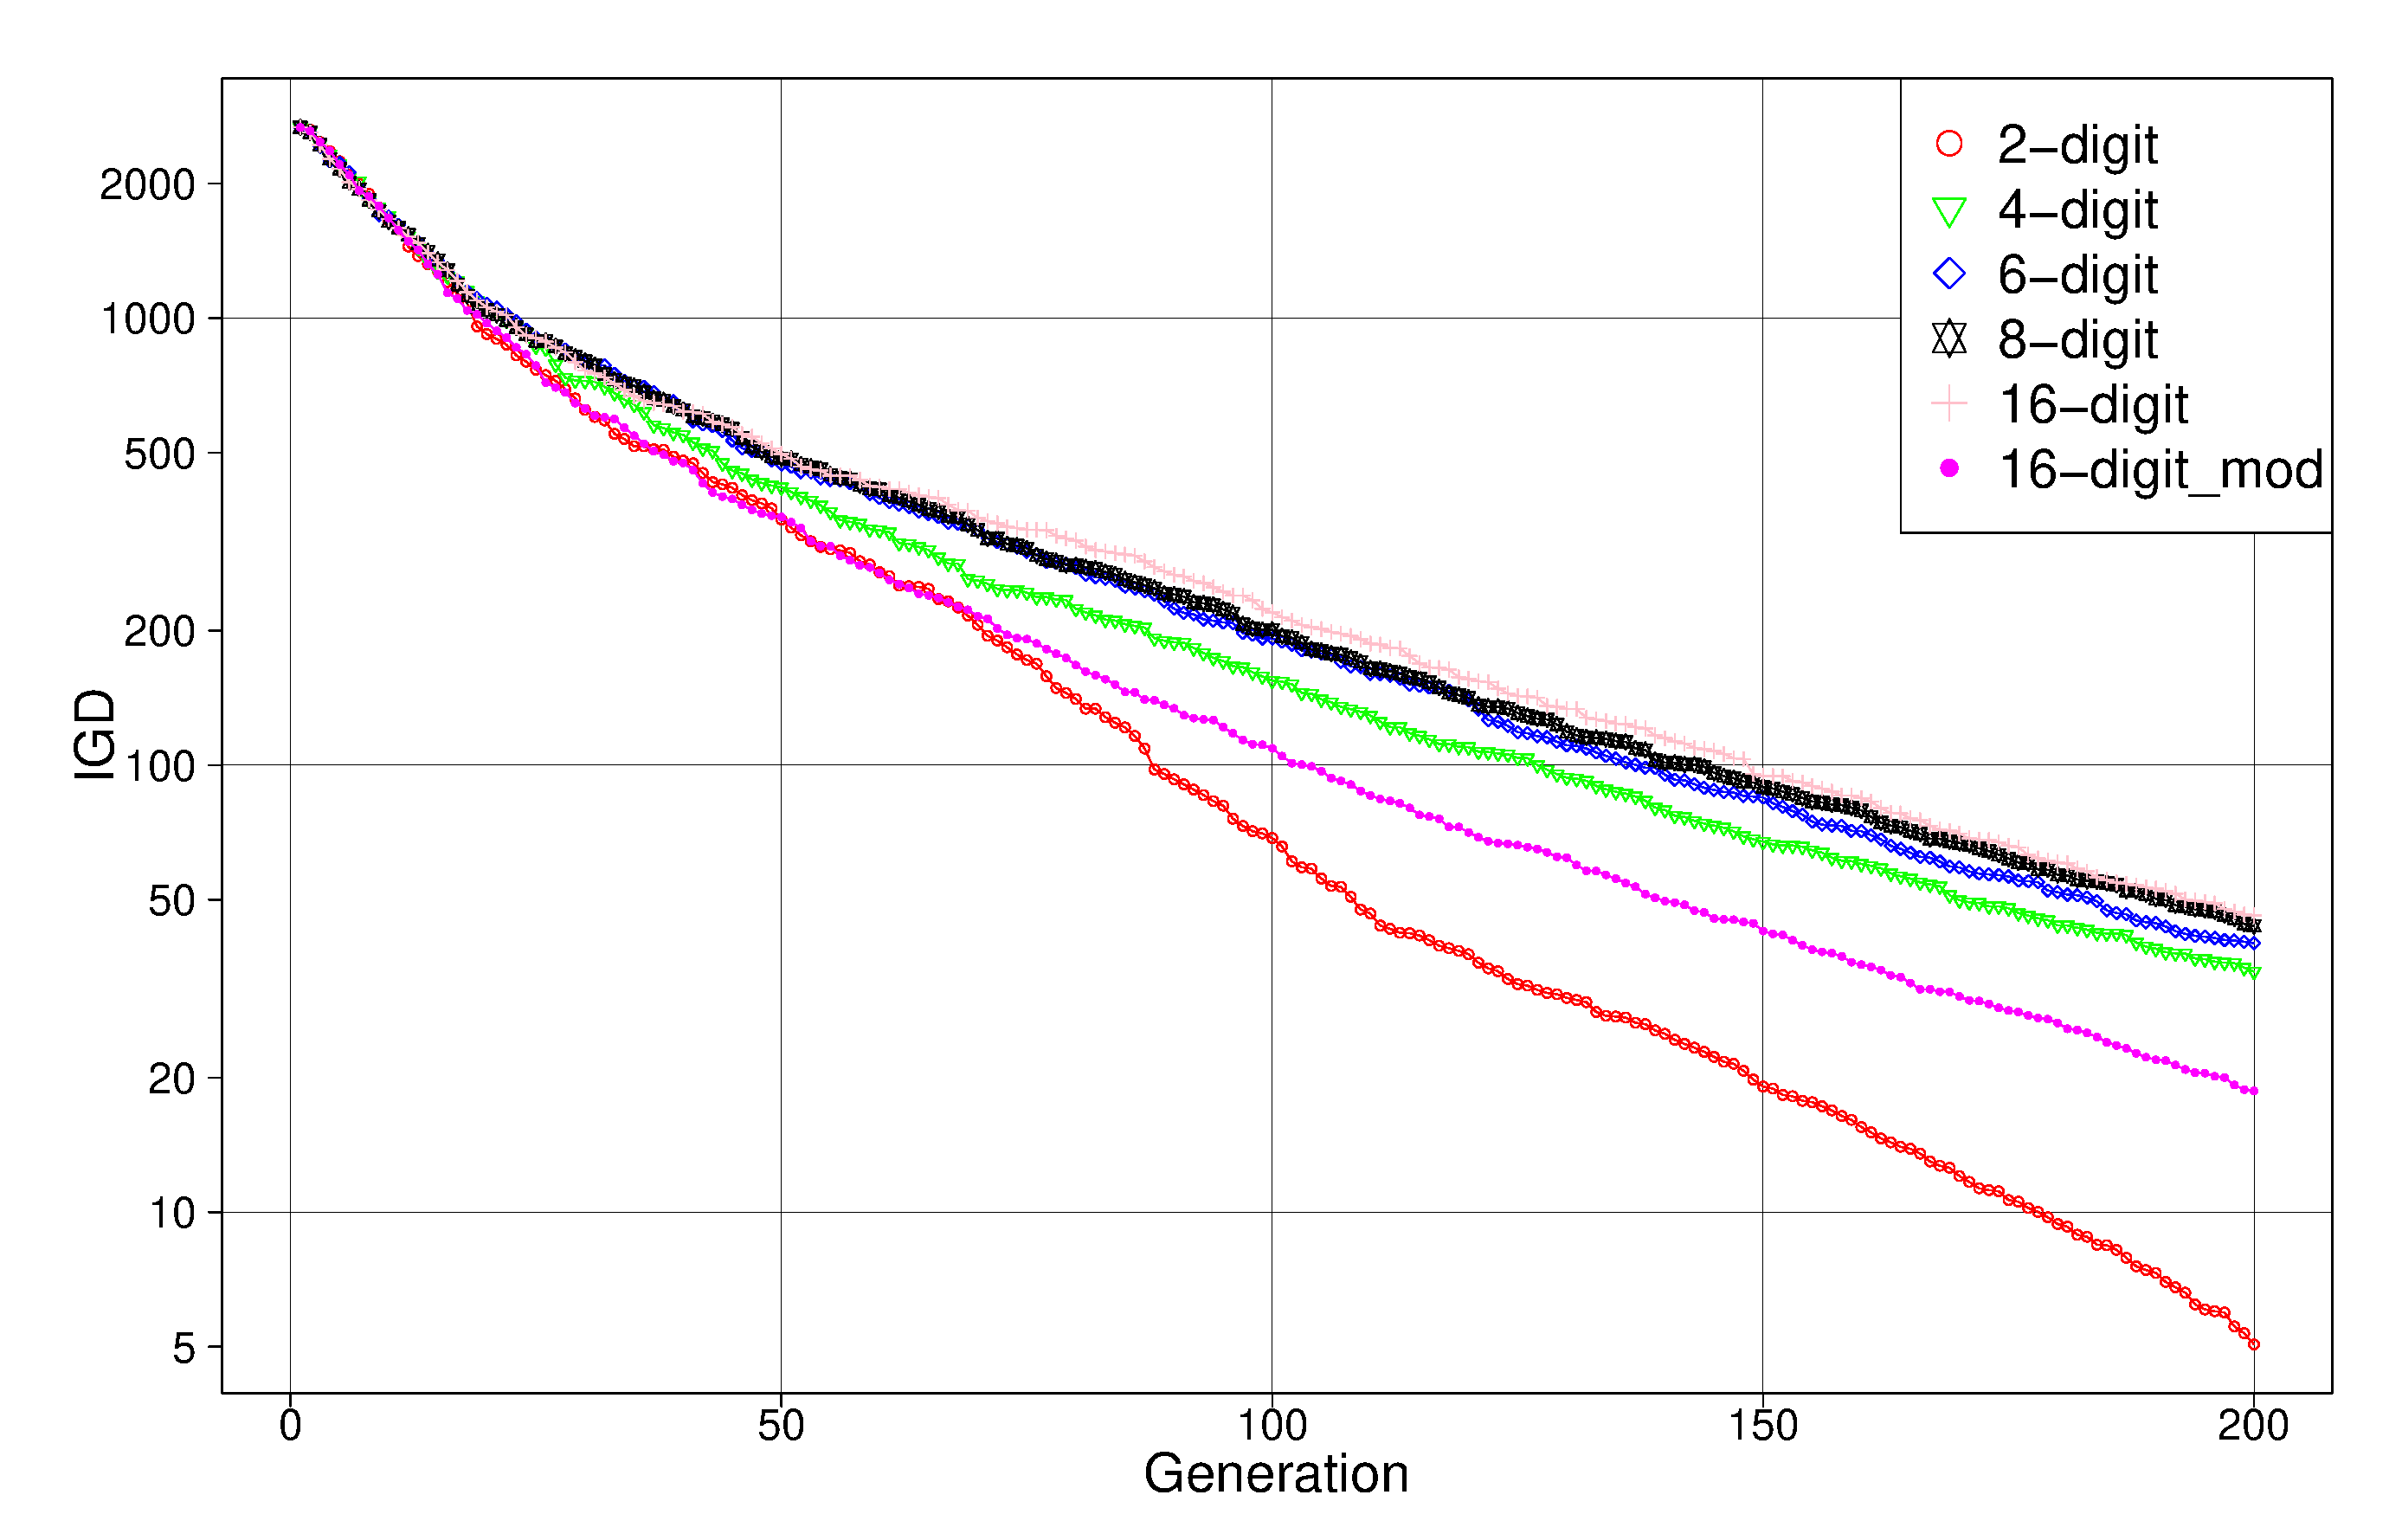
\includegraphics[width=1\linewidth]{../figures/DTLZ3_modified_IGD.eps}
%\setlength{\abovecaptionskip}{-8mm}
%\setlength{\belowcaptionskip}{-5mm}
%\caption{a}
\begin{center}
{\footnotesize (b) History of IGD}
\end{center}
\end{minipage}
\begin{minipage}{0.32\hsize}
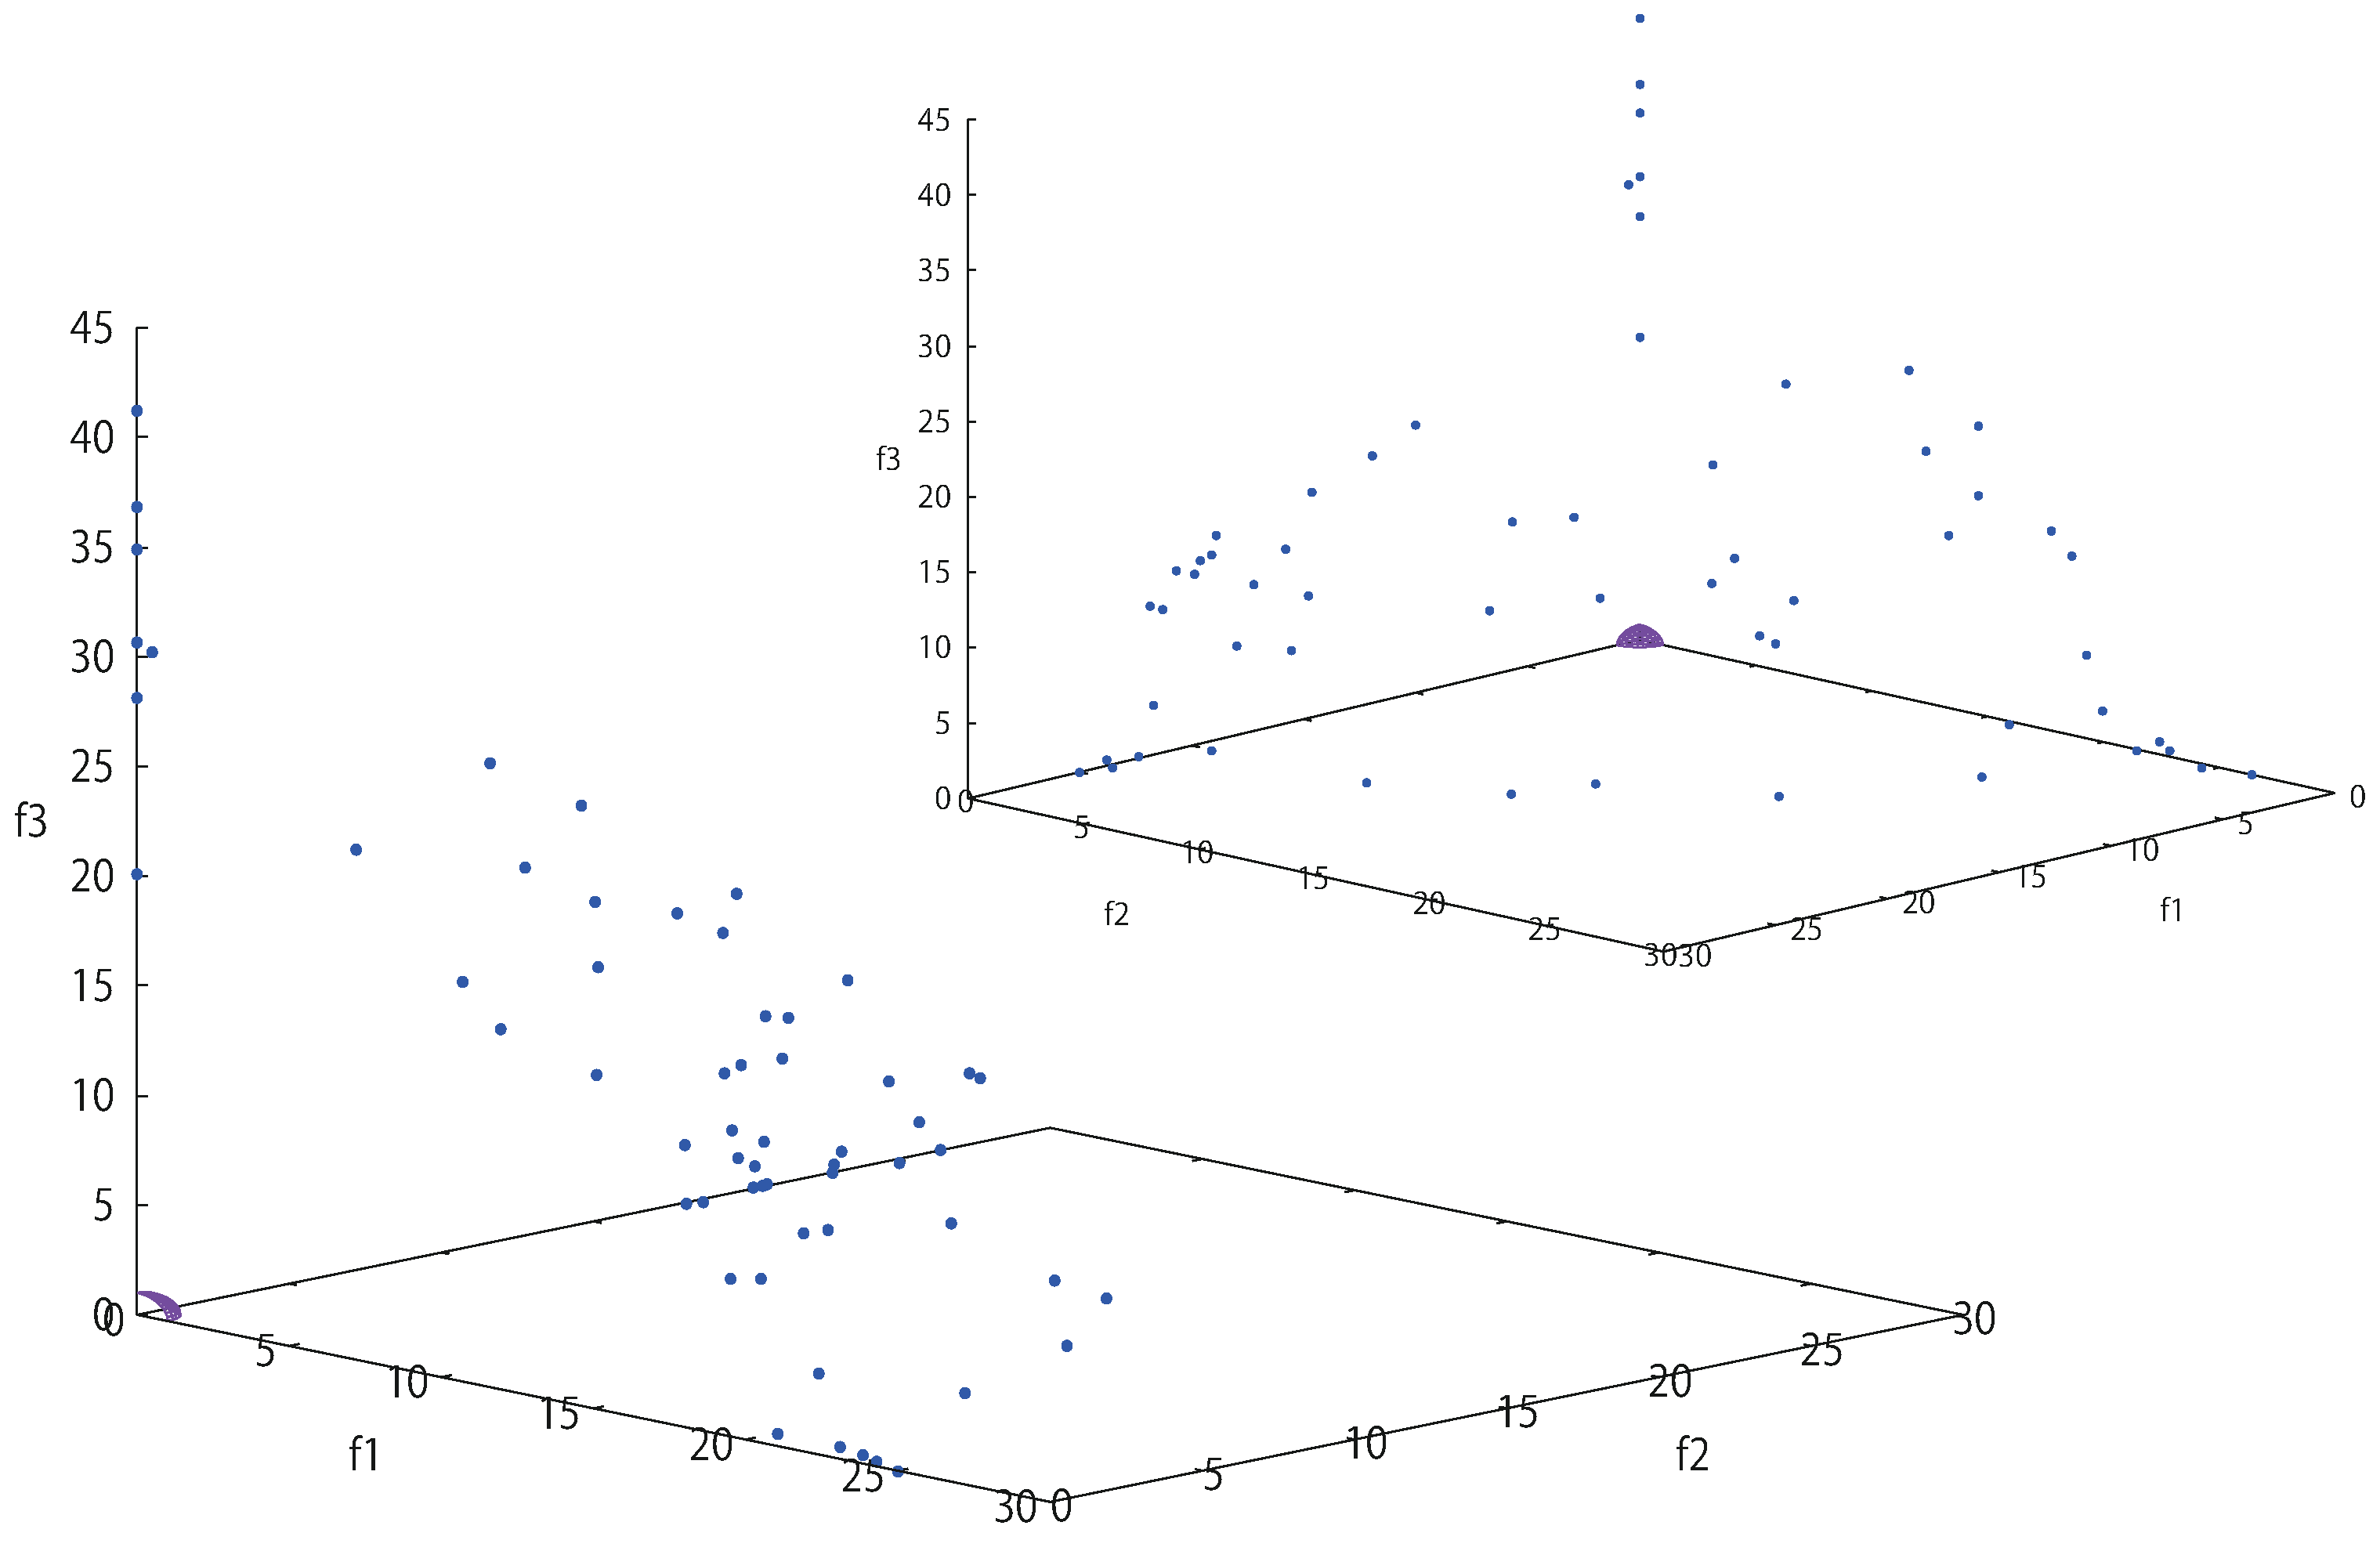
\includegraphics[width=1\linewidth]{../figures/DTLZ3mod_double.pdf}
%\setlength{\abovecaptionskip}{-8mm}
%\setlength{\belowcaptionskip}{-5mm}
%\caption{a}
\begin{center}
{\footnotesize (c) modified 16-digit}
\end{center}
\end{minipage}
\end{tabular}
\caption{Modified MethodにおけるGD,IGDの推移と非劣解集合}%GD / IGD histories and plots of final non-dominated individuals in the case of using modified 16-digit on DTLZ3.
\label{fig:mod}
%\setlength\textfloatsep{-5mm}
\end{figure*}
%
\clearpage
%
%\end{description}

\begin{description}
\item[{\large DRSs}]\mbox{}\\
\quad NSGA-IIなどの,解の優越性に基づいて個体を評価する最適化アルゴリズムでは,解空間の極付近に存在する解が,非劣解として生存しやすくなる.
このような解は,他の個体に支配されにくく,他の非劣解より収束が悪くても生存しやすい.DRSsとは,非劣解の中でも収束性が悪いにも関わらず,長い世代淘汰されずに残り続ける解のことである.
DRSsのイメージを図 \ref{drs} に示す.

\begin{figure}[htbp]
\begin{center}
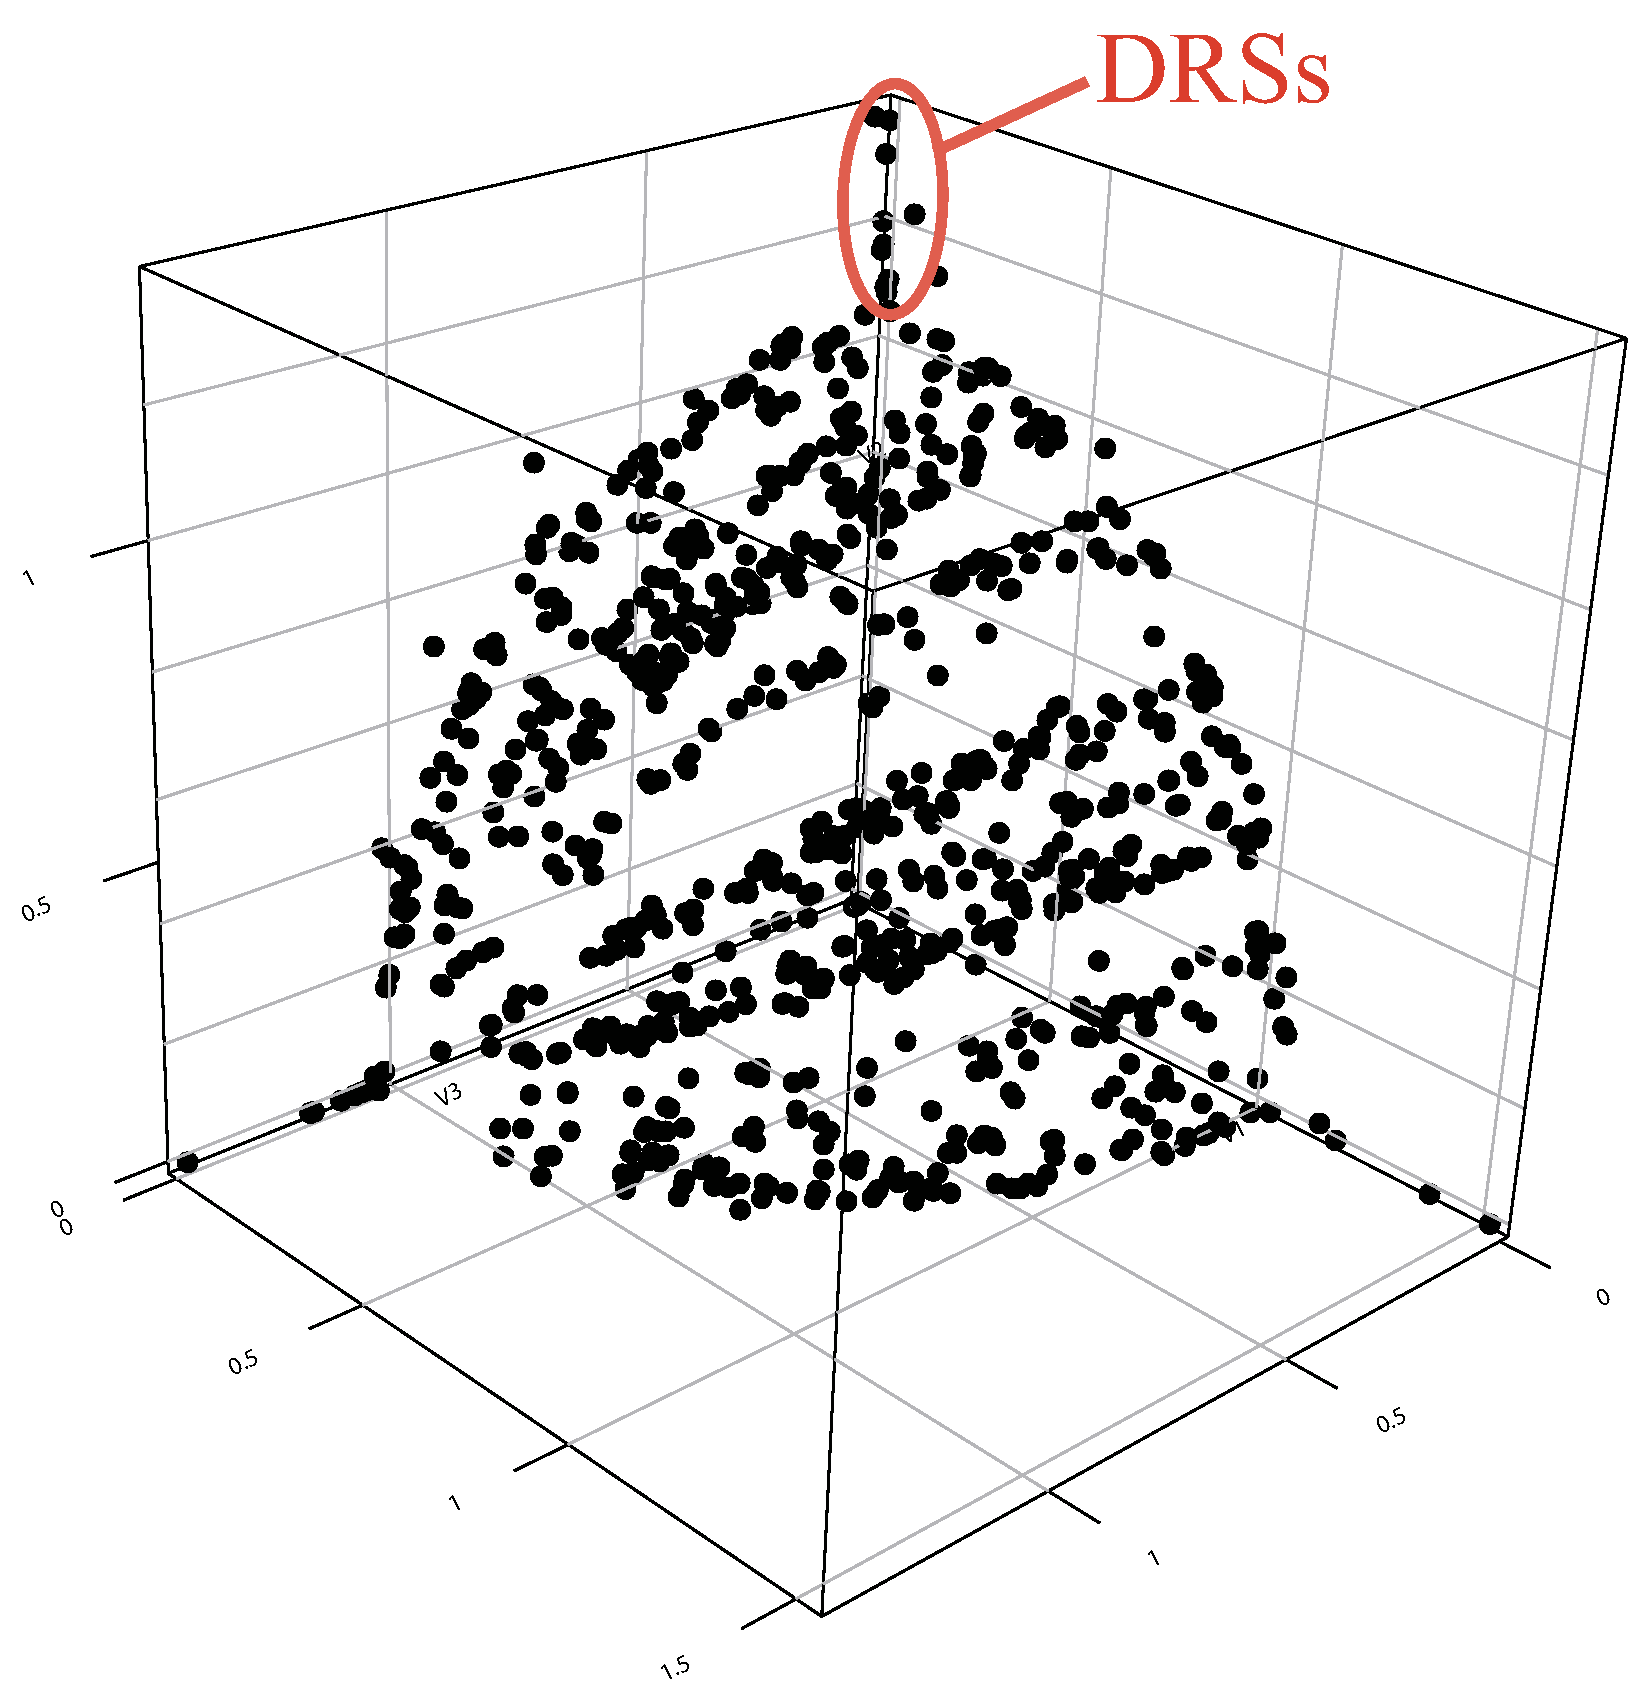
\includegraphics[width=0.7\linewidth]{../figures/DRSs.eps}
\end{center}
\setlength{\abovecaptionskip}{0mm}
\setlength{\belowcaptionskip}{0mm}
\caption{DRSsのイメージ図}
\label{drs}
\end{figure}

DRSsが多く存在すると,その周辺に次の個体が多く生成されるため,進化の効率が悪くなってしまうことが知られている.
\end{description}
%%\clearpage
%
\end{description}

\end{document}